





 



\documentclass[a4paper, 11pt]{book}



\usepackage{longtable}




\usepackage{geometry}% damit im Beispiel mehr Platz ist

\include{xcolor}






\usepackage{alltt}

\usepackage{tabularx}

\usepackage{ngerman, fancyheadings}

\usepackage{makeidx}



\usepackage{listings}


\usepackage[german,refpage]{nomencl}



\usepackage[utf8]{inputenc}

\usepackage{amsmath}

\usepackage{tikz}

\usepackage{graphicx}

\usepackage{mdframed}


\usepackage{thmtools}
\renewcommand*{\listtheoremname}{Liste der Sätze, Definitionen und Beispiele}

\usepackage[T1]{fontenc}

\usepackage{lmodern}




\usepackage[numbers]{natbib}

\usepackage[all]{nowidow}
\usepackage[citecolor=green,urlcolor=black,linkcolor=red]{hyperref}
\hypersetup{colorlinks=true}
\lstset{ language={java}, basicstyle=\ttfamily\footnotesize, breaklines=true, numbers=left, stepnumber=5, numberstyle=\tiny\color{gray}, mathescape=true, showstringspaces=false, inputencoding=utf8}

\newtheorem{Def}{Definition }[section]
\newtheorem{Pro}{Proposition}[section]
\newtheorem{Bsp}{Beispiel}[section]

\makeindex
\makenomenclature
% Längendefinitionen
\newlength{\currentLongTableWidth} %jeweils lokal anpassen
%\setlength{\currentLongTableWidth}{\textwidth} %setze neue länge auf textbreite
%\addtolength{\currentLongTableWidth}{-6\tabcolsep} %subtrahiere -8\cdot textbreite von asdf, 2 Abstände pro Zelle * Anzahl der Spalte



\begin{document}


\begin{titlepage}
\thispagestyle{empty}
\begin{center}
\Large{Fernuniversität Hagen}\\
\Large{Fakultät für Mathematik und Informatik}\\
\Large{Lehrgebiet Wissensbasierte Systeme}\\[1.5cm]
\end{center}


\begin{center}
{Arbeit im Diplomstudiengang Informatik (Diplom I)}\\[2.0cm]
\end{center}

\begin{center}


\LARGE \textbf{Ein Ansatz zur Beantwortung von Anfragen mit Variablen in der probabilistischen Konditionallogik FO-PCL}\\[3.5cm]
\end{center}


\begin{center}
\large{von Birgit Klaiber}\\[3.5cm]
\end{center}

\begin{center}
\large{Prüfer: Professor Dr. Christoph Beierle }\\[1.0cm]
\end{center}

\begin{center}
\textcolor{blue}{Version 20180513}
	
\large{Kleingartach, 2018}
\end{center}

\end{titlepage}






\begingroup


\pagenumbering{roman}

\setcounter{tocdepth}{1}

\tableofcontents
\clearpage
\endgroup
\pagenumbering{arabic}
\pagestyle{plain}
\setcounter{page}{1}
\pagestyle{headings}


\setlength{\parskip}{5pt}




\chapter{Einleitung}

\section{Allgemeines}

Wenn man die menschliche Fähigkeit aus vorhandenem Wissen intelligente Schlüsse folgern zu können, nachbilden möchte, steht man vor vielfältigen Problemen. Menschen schließen auf Basis von Erfahrungen und vorhandenen Informationen. Dieses Wissen ist in den seltensten Fällen sicher und meist auch nicht vollständig. Zur Nachbildung menschlicher Intelligenzleistungen müssen Systeme, die der Repräsentation und Verarbeitung realen Wissens dienen, damit umgehen können.

Um menschliches Schließen nachzubilden, versucht man es in einer abstrakteren Form zu charakterisieren. Unter Inferenz versteht ganz allgemein die Ableitung neuen Wissens aus vorhandenem Wissen. Vorhandenes Wissen und neu abgeleitetes Wissen sind durch eine Inferenzrelation miteinander verbunden 
\cite[S. 20]{BKI08}.

Gegenstand dieser Arbeit ist die Entwicklung und Implementierung einer neuartigen Inferenzkomponente, welche auf der probabilistischen Konditionallogik \footnote{Was man unter probabilistischen Konditionalen versteht wird im Anhang \ref{probKond} erklärt } First-Order Probabilistic Conditional Logic FO-PCL \index{FO-PCL} beruht. Eine ausführliche Beschreibung von FO-PCL finden sich in \cite[Kap. 6]{Fis10}. 

\section{Motivation und Problemstellung}

Eine gute Methode Unsicherheit quantitativ darzustellen, ist die Wahrscheinlichkeitstheorie. Ein Problem dabei ist, dass probabilistische Logik im Gegensatz zur klassischen Logik nicht wahrheitsfunktional ist, sich der Wahrheitswert einer Formel nur bei Unabhängigkeit  eindeutig aus den Wahrheitswerten der Teilformeln bestimmt. Daher ist es notwendig, um wahrheitsgemäß schließen zu können, ausreichende Informationen zu besitzen. Dieses Wissen zu ermitteln ist nicht immer einfach und oft sehr aufwendig. Man suchte daher Methoden, probabilistisches Wissen möglichst informationsgetreu durch verfügbares Wissen anzureichern. 

Wissensrepräsentationen der realen Welt erfordern es nicht nur, unsicheres Wissen über ein bestimmtes Objekt darzustellen, sondern über eine Vielzahl verschiedener Objekte und deren ggf. unsichere Beziehungen, vgl. \cite[S. 19]{Fis09}
Beschränkt man sich auf aussagenlogisches konditionales Wissen und dessen Verarbeitung, lassen sich manche Zusammenhänge der realen Welt gar nicht oder schwer darstellen oder nur durch redundante und gegebenenfalls unnötige Berechnungen. Die (propositionale) probabilistische Konditionallogik Probitional Conditional Logic (PCL) \index{PCL} ist ein Beispiel für eine Logik, die die Gegebenheiten der realen Welt abbilden kann und das auf relativ unkomplizierte Weise. Ausführliche Anmerkungen zu PCL finden sich in \cite{RKI96} und in \cite[Kap. 2.4]{Fis10}. 

\begin{Bsp}[Grippe]\label{sec:Bsp1}\
Das Beispiel "{}Grippe"{} beschreibt das unsichere Wissen bezüglich der Ursachen einer Ansteckung mit Grippe. Es wurde aus \cite[Bsp. 6.2.7, S. 128/129]{Fis10} entnommen und leicht modifiziert.

Im Allgemeinen sind Menschen nur mit geringer Wahrscheinlichkeit an Grippe erkrankt. Wenn jemand anfällig für eine Grippeerkrankung ist, erkrankt er mit höherer Wahrscheinlichkeit an Grippe als andere Personen. Weiterhin gilt, wenn eine Person A mit einer Person B Kontakt hatte und A an Grippe erkrankt ist, ist es wahrscheinlicher, dass B an Grippe erkrankt. 

Wenn wir uns nun auf den aussagenlogischen probabilistischen konditionalen Fall beschränken und in diesem Fall PCL \index{PCL} verwenden würden, könnte das wie folgt aussehen:\\
\\
Sei $ \cal{R} $$_{Gr}  $ = $ (Gr_{1}, Gr_{2}, Gr_{3})  $ eine PCL Wissensbasis mit den Konditionalen 
\begin{quote}
$ Gr_{1}  :  \langle (AGr)[0,01]\rangle $,\\
$ Gr_{2} : \langle (AGr \mid Aan)[0,1]\rangle$\\
$ Gr_{3} : \langle (BGr \mid KAB \wedge AGr )[0,6]\rangle$\\
\end{quote}
wobei:\\
AGr die Aussage darstellt, dass Anna an Grippe erkrankt ist, Aan der Aussage entspricht, dass Anna anfällig für Grippe ist und KAB der Aussage entspricht, dass Anna und Bob Kontakt hatten und BGr der Aussage, dass Bob an Grippe erkrankt ist. 
\\
\\
Jetzt möchte man nun nicht für jede mögliche Person der realen Welt eine eigene Aussage erstellen, sondern den allgemeinen Fall beschreiben.
\\
Sei $ \cal{R} $$_{GrFO} $ = $ (GrFO_{1}, GrFO_{2}, GrFO_{2})  $ eine FO-PCL Wissensbasis mit den Konditionalen 
\begin{quote}
$ GrFO_{1}  :  \langle (Gr(X))[0,01], \top \rangle $,\\
$ GrFO_{2} : \langle (Gr(X) \mid An(X)[0,01], \top \rangle$\\
$ GrFO_{3} : \langle (Gr(Y) \mid Kon(X, Y) \wedge Gr(X )[0,6], X \neq Y \rangle$\\
\end{quote}
wobei:\\
die Menge der Prädikate $Präd_{GrFO}$  = \{ Gr(X), An(X), Kon(X, Y),$ \top $    und $ \bot  $ und $ =^{(s)}$ \}, wobei Gr(X) bedeuten soll X ist an Grippe erkrankt, An(X) X ist anfällig für Grippe und Kon(X, Y),  X hatte Kontakt mit Y. $ \top $ steht für die Tautologie und $ \neq  $ ist das Prädikatensymbol für die Ungleichheit von Termen\footnote{das nur in den Constraints verwendet wird (wird unten näher beschrieben)} besteht. Dieses Beispiel dient dazu, die Grippeansteckungsmechanismen zu beschreiben. Der Constraint $  "{} X \neq Y "{} $ dient der Vermeidung von Inkonsistenzen.


\end{Bsp}

\begin{Bsp}[Sympathie]\label{sec:BspSmp}\
Man möchte modellieren, dass in einer Gruppe von Personen bestimmte Sympathien herrschen.

Im aussagenlogischen probabilistischen konditionalen Fall könnte man die Aussage, dass eine Person Anna eine Person Bob mag mit AmB beschreiben. Wenn Anna Bob mag, dann mag Bob auch Anna (BmA) mit einer hohen Wahrscheinlichkeit.
Mit PCL Konditionalen ausgedrückt, könnte das so aussehen:
\begin{quote}
$ S_{1} : \langle (BlA \mid AlB)[0,9]\rangle$\\
\end{quote}
Wenn unsere Personengruppe mehr Personen enthält, wollen wir vielleicht den allgemeinen Fall modellieren, der besagt, dass Sympathie mit hoher Wahrscheinlichkeit auf Gegenseitigkeit beruht.
Mit FO-PCL Konditionalen ausgedrückt:
\begin{quote}
	$ S_{2} : \langle (likes(U, V) \mid likes(V, U)[0,9], U \neq V \rangle$\\
\end{quote}

\end{Bsp}

\begin{Bsp}[Misanthrope (Idee)]\label{sec:Misanthrop}\
Man kann nun das Beispiel \ref{sec:BspSmp} "{}Sympathie"{} um ein weiteres Konditional erweitern, welches besagt, dass es in der (endlichen) Gruppe einen Misanthropen gibt, identifiziert mit dem Konstantensymbol a, der nur selten Sympathie empfindet. Das Beispiel "{}Misanthrope"{} wurde \cite[Bsp. 6.5.3, S. 144]{Fis10} entnommen. Eine ausführlichere Version dieses Beispieles findet sich unter \ref{Bsp:Misanthrope} und \ref{Misanthrope}.
\begin{quote}
$ MI_1 : \langle (likes(U, V) \mid likes(V, U)[0,9], U \neq V \rangle$\\
$ MI_2 : \langle (likes(a, V))[0,05], V \neq a \rangle$\\
\end{quote}


\end{Bsp}
FO-PCL\index{FO-PCL} wird in \cite[Kap. 6]{Fis10} präsentiert und eröffnet eine Möglichkeit, den Zweck der Verbindung von Wissensrepräsentation und (Prädikaten-)Logik erster Stufe zu erfüllen und gleichzeitig Nachteile anderer bekannter Ansätze, die im folgenden noch erwähnt werden, zu kompensieren.     

                            
Wie in \cite[S. 19]{Fis09} erläutert wird, stellen probabilistische graphische Modelle in Verbindung mit einer Teilmenge der (Prädikaten-)Logik den geläufigsten Formalismus dar, um Wissensrepräsentation und Logik zu verbinden; einen Überblick darüber kann man sich \cite{SBAR08} und in \cite[Kap. 10]{GT07} verschaffen. Bekannteste Vertreter der probabilistischen graphischen Modelle sind Markov Logic Networks (MLNs), Bayes Logic Programs (BLPs) und Probabilistisch Relationale Modelle (PRMs). Sie finden erfolgreich in verschiedenen Bereichen praktische Anwendung.
Nähere Informationen zu den Konzepten und ihrer Anwendung entnehmen sie bitte den entsprechenden Kapitel in \cite{GT07}.

Dabei ist die bedingte Unabhängigkeit das fundamentale und entscheidende Prinzip probabilistischer Netze. Mit einem Bayes- oder Markov-Netz modelliert man in erster Linie Unabhängigkeiten, s. auch \cite[Kap. 12.1 und 12.2]{BKI08}. Um ein entsprechendes Netz aufbauen zu können, ist es notwendig, die Zusammenhänge zu betrachten. Allerdings ist die Beurteilung von Abhängigkeiten und Unabhängigkeiten der einzelnen Variablen so schwierig, dass selbst Experten unter Umständen zunächst keine eindeutige Aussage machen können, wie sich die Variablen zueinander verhalten. Zur Ermittlung der Zusammenhänge ist daher unter Umständen ein erheblicher statistischer Aufwand nötig, vgl. \cite[12.6, S. 402 /403]{BKI08}.
 Ein weiteres Problem ist, dass MLNs, da sie ungerichtete Graphen mit Prädikatenlogik kombinieren und dabei gewichtete Formeln nutzen, schwer verständlich und schwer zu spezifizieren sind. Nähere Ausführungen zu MLNs können \cite{DR06} entnommen werden. 
 
 BLPs dagegen nutzen gerichtete Graphen in Kombination mit Logikprogrammen. Bayes Netze können kausale Abhängigkeiten darstellen, die Modellierung eines Bayesschen Netzes erfordert einige Mühe und bringt ein sehr effektives, aber auch starres probabilistisches Gerüst hervor. Durch die Struktur des Netzes und die angegebenen Wahrscheinlichkeiten wird die Verteilung vollständig bestimmt. Bayessche Netze können keine allgemeinen Abhängigkeiten, das sind Abhängigkeiten, die nicht notwendig kausal bzw. bedingte Unabhängigkeiten sind, darstellen. Sie können keine zyklischen Wirkungen repräsentieren. Kausale Abhängigkeiten sind aber in bestimmten Einsatzbereichen \footnote {wie zum Beispiel der Auswertung sozialer Beziehungen}, welche eher durch Korrelation gekennzeichnet sind, nicht gegeben.
 
Einen kurzen Überblick über MLNs und BLPs liefert \cite[Kap. 2.1 und 2.2]{FLT09}.
Ausführlichere Anmerkungen dazu finden sich auch in \cite[Kap. 2]{KIBFT11}.

Die probabilistische Konditionallogik PCL \index{PCL} \nomenclature{PCL}{Probabilistische Konditionallogik} erlaubt eine Repräsentation unsicheren Wissens, in dem sie ermöglicht,  unsichere Fakten und unsichere wenn-dann Regeln, so genannte Konditional, welche je mit einem bedingten Wahrscheinlichkeitswert parametrisiert sind, darzustellen. 

Da sie aber auf Aussagenlogik beruht, beschränkt man sich in der Mächtigkeit der Ausdrucksfähigkeit (s. auch obiges Beispiel \ref{sec:Bsp1}) "{}Grippe"{}. Die Erweiterung von PCL auf den Fall einer Vielzahl von Objekten und deren allgemeiner Beziehungen, also um die Prädikatenlogik erster Stufe, führte zu FO-PCL.

Die Nachteile probabilistisch graphischer Modelle lassen es somit sinnvoll erscheinen, einen anderen Formalismus zu betrachten, der den Anforderungen der realen Welt  gerecht wird, indem er unsicheres Wissen quantifiziert, gleichzeitig aber die genannten Nachteile möglichst vermeidet. Um die reale Welt repräsentieren zu können, muss man mit Unsicherheit umgehen können. Man muss mit vielen (verschiedenen) Objekten und deren möglichen, eventuell auch unsicheren,  Beziehungen zueinander umgehen und sie verarbeiten können.

FO-PCL ist es im Gegensatz zu den probabilistischen Netzwerken wie BLPs, und MLNs möglich, allgemeine Abhängigkeiten (nicht notwendig kausale Abhängigkeiten bzw. bedingte Unabhängigkeiten, vgl. auch obiger Abschnitt) darzustellen. Sie ermöglicht Wissensrepräsentation und Inferenz auf der Basis des verfügbaren, auch unvollständigen probabilistischen Wissens. 


\section{Gegenstand und Ansatz}
Um unsicheres Wissen adäquat darstellen und verarbeiten zu können, bieten sich aussagenlogische Konditionale \index{Konditional} an, welche bedingte Abhängigkeiten darstellen. Eine Erweiterung von aussagenlogischen, probabilistischen Konditionalen auf Basis der Prädikatenlogik erster Stufe wird in \cite[Kap. 6]{Fis10} beschrieben.

 Die Semantik von FO-PCL basiert auf dem Konzept der maximalen Entropie und ist mittels der Menge aller Grundinstanzen\footnote{sh. Definition \ref{Grundinstanz}} eines Konditionals definiert. Ein Constraint, der einem Konditional zugeordnet wird, schränkt dabei die zulässigen Grundinstanzen eines Konditionals ein, um Inkonsistenzen in der Menge aller Grundinstanzen zu vermeiden.
 
Inferenz erfolgt auf aussagenlogischer Ebene, d.h. um neues Wissen abzuleiten, betrachtet man die Grundinstanzen der Konditionale.


Die Aufgabenstellung dieser Diplomarbeit beinhaltet den Entwurf und die Implementierung einer Inferenzkomponente für FO-PCL unter Verwendung bereits vorhandener Komponenten der Bibliothek Log4KR, eines Projektes der FernUniversität Hagen. Dabei soll die Inferenzkomponente qualitative Konditionale, das sind Konditionale ohne Wahrscheinlichkeit, als Anfrage entgegennehmen und diese mit einer zugeordneten Wahrscheinlichkeit zurückliefern. Es sollen Äquivalenzklassen   aus den Grundinstanzen\footnote{sh. Definition \ref{Grundinstanz}}  des angefragten Konditionals gebildet werden, die die Grundkonditionale\footnote{sh. Definition \ref{Generalisierung}} mit gleichem Parameterwert zu möglichst allgemeinen Konditionalen zusammenfassen \footnote{Eine Definition des Begriffes und nähere Erläuterungen finden sich in \ref{Äquivalenzklassen}}. Dabei wird darauf geachtet werden, so wenig Äquivalenzklassen wie möglich zu bilden, sich gleichzeitig aber nicht in der Ausdrucksfähigkeit der Informationen der Wissensbasis zu beschränken.

Die wesentliche Aufgabe dieser neuen Inferenzkomponente ist es, das vorhandenes Wissen zu nutzen, auszuwerten und Schlüsse zu ziehen.\\
Sie erlaubt die indirekte Kommunikation mit dem Anwender über eine Schnittstelle, nimmt Anfragen entgegen, bereitet sie gemäß der Semantik von FO-PCL auf, zieht die notwendigen logischen Schlüsse und nimmt unter Verwendung von bereits in Log4KR vorhandenen Komponenten die erforderlichen Berechnungen.
 
\includegraphics[scale = 0.6]{Graphics/Ablauf}
\begin{figure}[h]
	\caption{Ablauf einer Anfrage}
	\label{Ablauf}
\end{figure}
 
Zunächst nimmt die Inferenzkomponente dafür ein qualitatives Konditional entgegen. Sie generiert die Grundinstanzen dieses Konditionals, d.h. falls das Konditional Variablen enthält, werden diese mit allen zulässigen Konstanten des Universums belegt. Zulässige Konstanten sind solche, deren Verwendung anstelle der Variablen zu einem Konditional führt, das konsistent mit der Wissensbasis ist. Danach berechnet die Inferenzkomponente zu jeder Grundinstanz die dazugehörige Wahrscheinlichkeit; unzulässige Belegungen\footnote{Das sind solche Belegungen, die durch einen Constraint ausgeschlossen wurden.}, werden dabei am Berechnungsergebnis erkannt. Anschließend fasst die Komponente Grundkonditionale mit gleicher (zulässiger) Wahrscheinlichkeit zu einem möglichst allgemeinen Konditional zusammen.

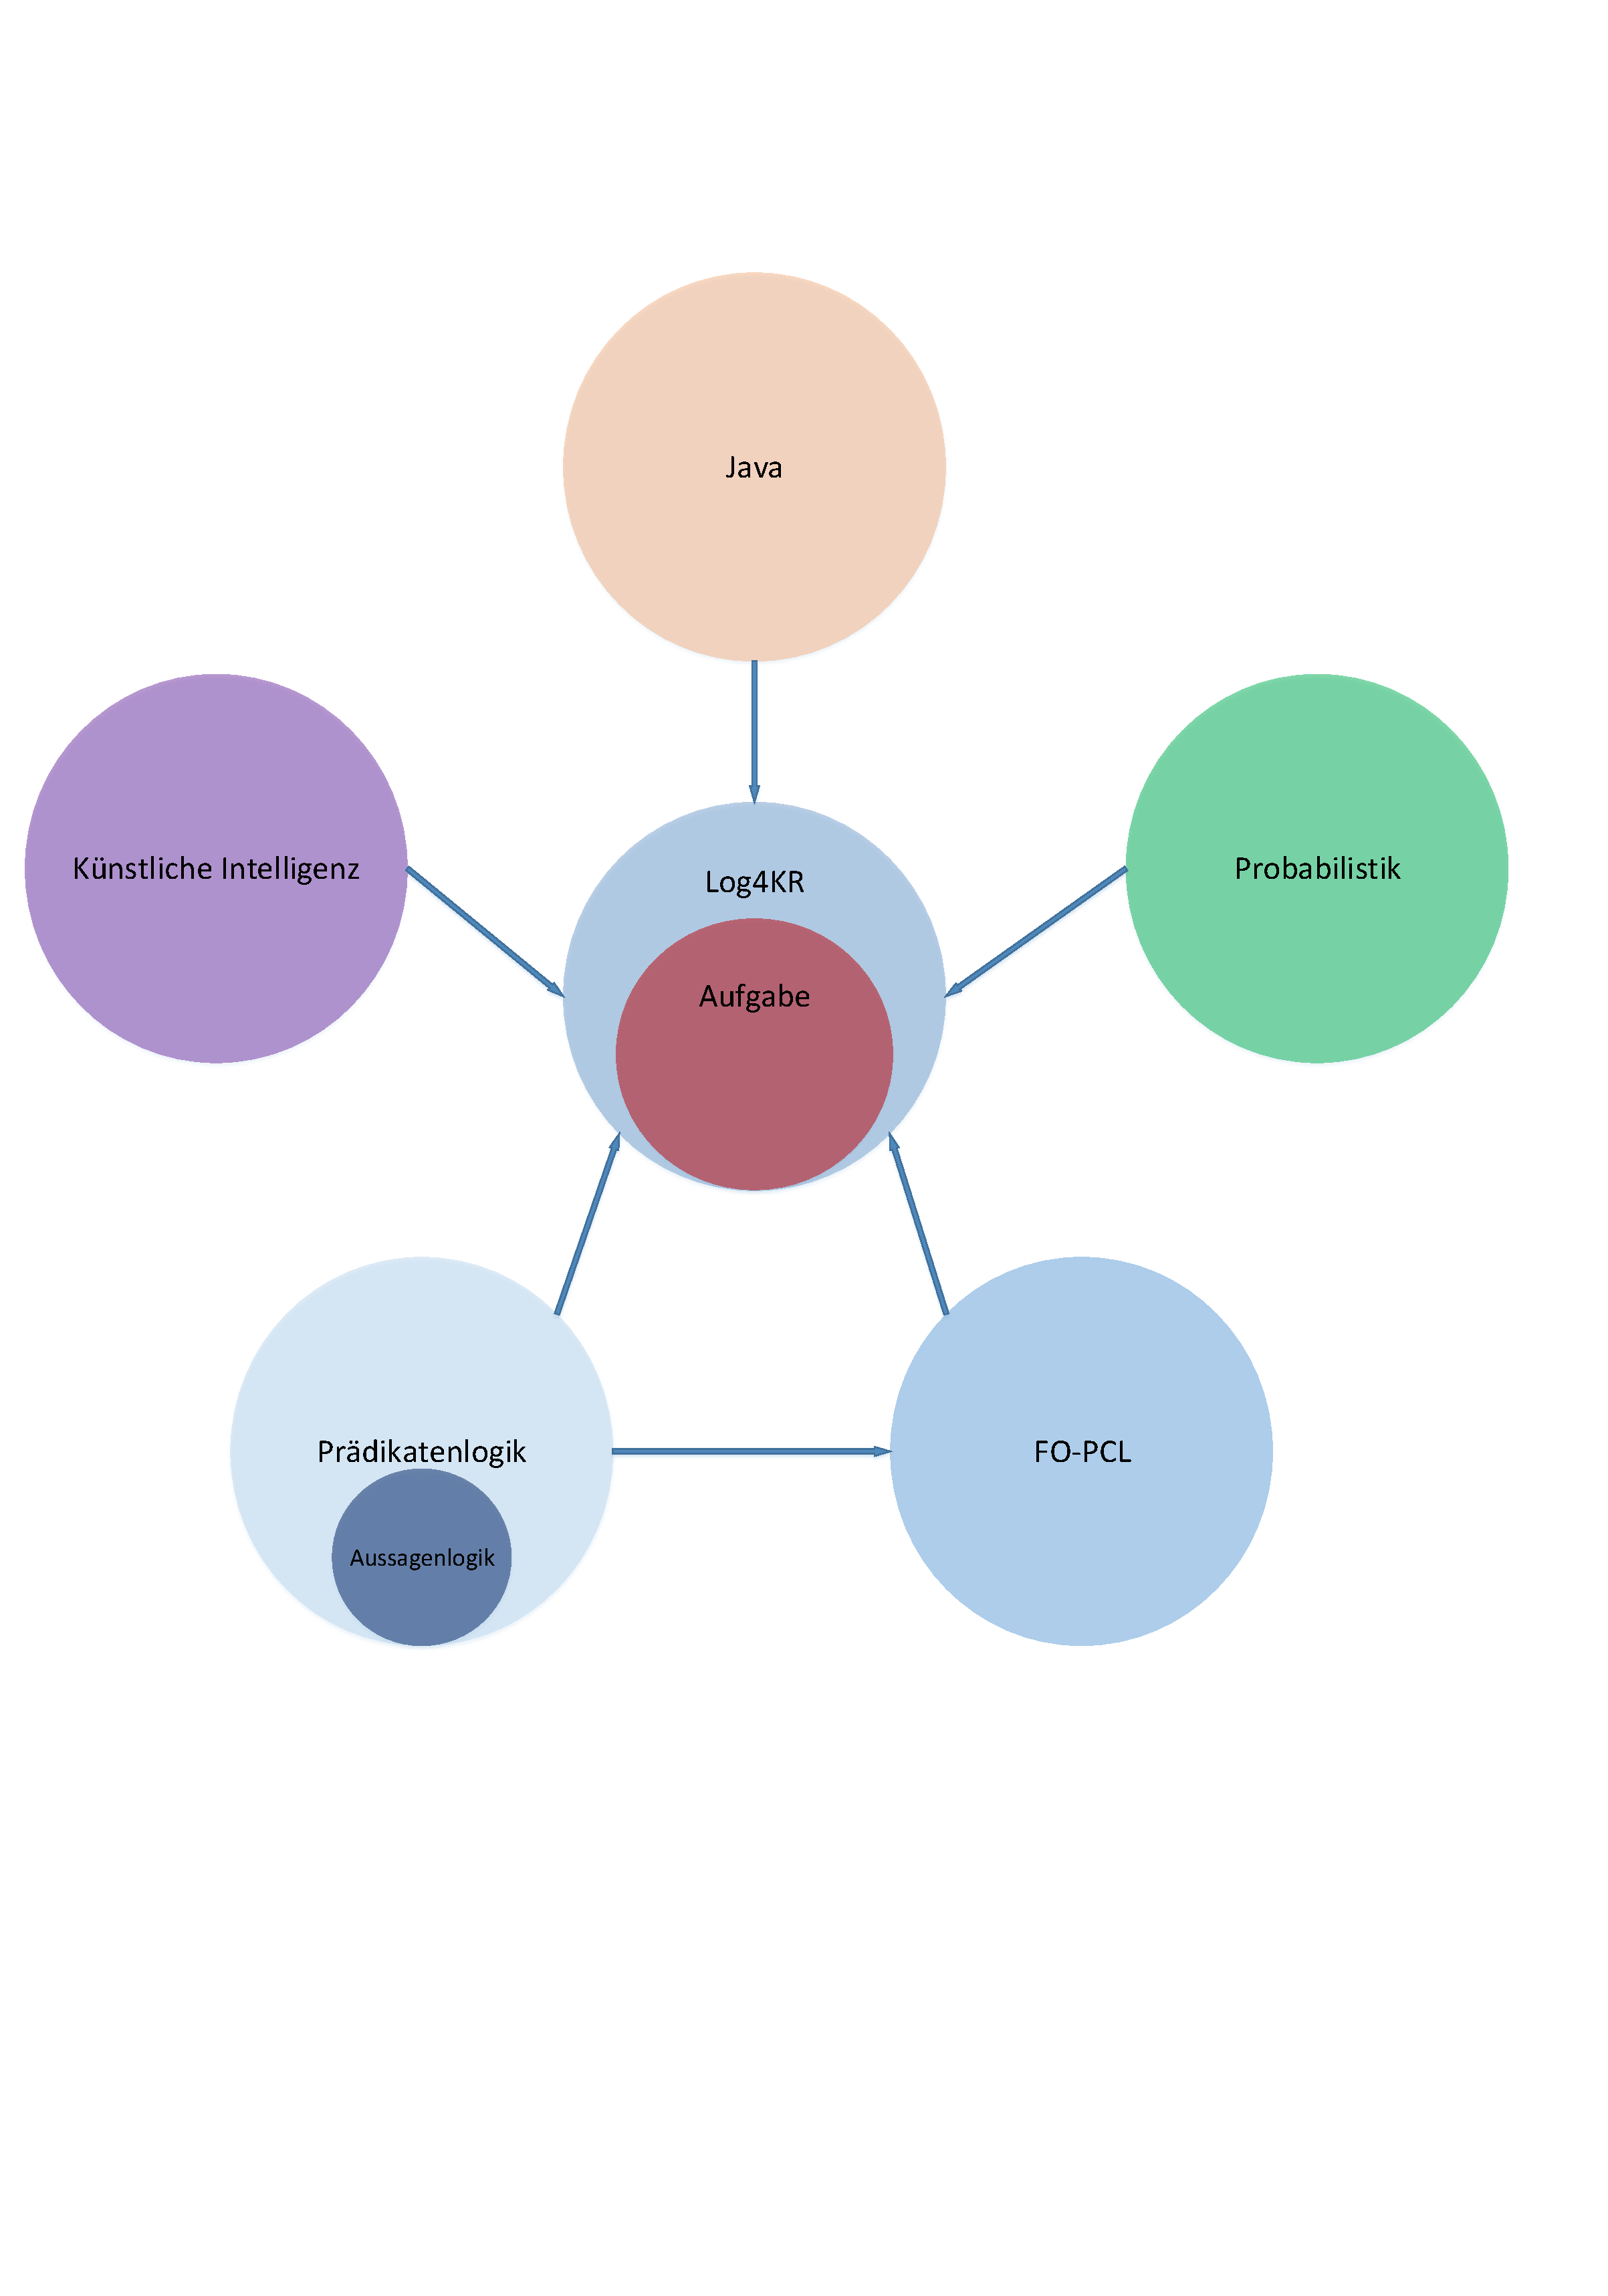
\includegraphics[scale = 0.3]{Graphics/Eingangsbild}
\begin{figure}[h]
	\caption{Einordnung des Themas und der Aufgabe}
	\label{Eingangsgrafik}
\end{figure}
\newpage

Mit den bisher vorhandenen Komponenten aus Log4KR ist es nur möglich, die Wahrscheinlichkeit zu einem qualitativen Grundkonditional zu erhalten. Das ist zwar hilfreich, wenn man ein Grundkonditional hat, wenn das Konditional jedoch Variablen enthält, kann man seither keine Wahrscheinlichkeit berechnen und ausgeben lassen.
Wenn man eine Menge von speziellen Konditionalen, die gemeinsame Eigenschaften besitzen erhalten kann, lässt sich das neu gewonnene Wissen viel besser erschließen. \\
Eine Einordnung des Themas kann der Abbildung 1 \ref{Eingangsgrafik} entnommen werden.


Zunächst wird in Kapitel \ref{FO-PCL} auf FO-PCL selbst eingegangen und diese ausführlich erläutert. Kapitel \ref{Inferenz} beschreibt den Inferenzprozess in FO-PCL. Die experimentellen Forschungen werden in Kapitel \ref{Experim. Forschungen} erläutert und in Kapitel \ref{Beob} ausgewertet. Ideen für Algorithmen werden in Kapitel \ref{Ideen Alg.} ausgeführt und diskutiert. Über die einzelnen Phasen der Entwicklung der Inferenzkomponente gibt Kapitel  \ref{Dok} Auskunft. Der entworfene Algorithmus wird in Kapitel \ref{Alg}  beschrieben. Die Implementation der Inferenzkomponente und der Inferenzprozess  und seine Erläuterung anhand von Beispielen ist Inhalt von Kapitel \ref{Inf}. 

 Die Korrektheit und Vollständigkeit des Algorithmus wird in Kapitel \ref{eval} empirisch belegt. Ergebnisse und Ausblick beschließen diese Arbeit in Kapitel \ref{Erg}. Im Anhang befinden sich die Erläuterungen verschiedener theoretischer Grundlagen.



\newpage

\chapter{FO-PCL}\label{FO-PCL} \nomenclature{FO-PCL}{probabilistische Konditionallogik erster Stufe}
Unter FO-PCL\index{FO-PCL} versteht man die Erweiterung von propositionalen (d.h. aussagenlogischen) Konditionalen (d.h. der PCL) auf Basis der Prädikatenlogik erster Stufe. Die Semantik basiert auf dem Konzept der maximalen Entropie (nähere Ausführungen können dem Anhang \ref{MaxEnt} entnommen werden) und ist mittels der Menge aller Grundinstanzen eines Konditionals definiert\footnote{Was unter einer Grundinstanz zu verstehen ist, wird im Folgenden noch ausführlich erläutert, Definition, sh. \ref{Grundinstanz} }. Ein Constraint \index{Constraint} (oder eine constraint Formel), das einem Konditional \index{Konditional} zugeordnet wird, dient dazu,  die zulässigen Grundinstanzen eines Konditionals einzuschränken.

\begin{Bsp}[Inkonsistenz]
\label{sec:Bsp}

Wenn man Beispiel \ref{sec:Bsp1} "{}Grippe"{} betrachtet, enthält das Konditional $ GrFO_{3}$ den Constraint der Ungleichheit $ "{} X \neq Y "{} $. Ohne diese Einschränkung könnte man X und Y mit der gleichen Konstante instantiieren und erhielte  für eine Menge $ \cal D $$_{GrFO} $ von Konstanten mit\\
 $ \cal D $$_{GrFO}  $ $ = \{Anna, Bob \} $ unter anderem die folgende Grundformeln:\\
 \begin{quote}
 	$ GrFO_{1, 1}  :  \langle (Gr(Anna))[0,01], \top \rangle $,\\
 	$ GrFO_{3, 1} : \langle (Gr(Anna) \mid Kon(Anna, Anna) \wedge Gr(Anna)[0,6]  \rangle$\\
 \end{quote}
  Was zu der Erkenntnis führen würde, dass Anna hat mit einer Wahrscheinlichkeit von 1\% gemäß  $ GrFO_{1, 1}  $ und mit einer Wahrscheinlichkeit von 60 \% gemäß $ GrFO_{3, 1}  $ an Grippe erkrankt ist. 
  
 D.h. es würde folgen, dass eine Person, die an Grippe erkrankt ist und mit sich selbst Kontakt hatte (was ja im realen Leben nicht unwahrscheinlich ist, alles andere wäre ein fast ausschließlich philosophische Frage), eine höhere Wahrscheinlichkeit hätte, an Grippe zu erkranken. Das wäre im realen Leben unsinnig und würde hier zu einer inkonsistenten Wissensbasis führen, da die beiden oben aufgeführten Konditionale unterschiedliches Wissen zum gleichen Atom (hier die unterschiedlichen Wahrscheinlichkeiten zu Gr(Anna), der Grippeerkrankung von Anna) enthielten, je nachdem welches Konditional man betrachtet. 



\end{Bsp}

\begin{Bsp}[Constraint]
\label{sec:BspConstraint}
Der Constraint $ "{} U \neq V "{} $ im Konditional $ S_{2} $ aus Beispiel \ref{sec:BspSmp} "{}Sympathie"{} dient der Vermeidung der Inkonsistenz, die aus der Instanziierung von X und Y mit der gleichen Konstanten entstehen würden und die besagten, dass sich jemand, der sich sicher mag mit einer hohen Wahrscheinlichkeit mag. 
\end{Bsp}
Constraints dienen dazu, Inkonsistenzen in der Menge aller Grundinstanzen zu vermeiden, vgl. Beispiel \ref{sec:Bsp1} "{}Grippe"{}  und \ref{sec:BspSmp} "{}Sympathie"{} oder um besonderes Wissen über bestimmte Objekte auszudrücken, was im Folgenden noch näher erläutert wird.


\section{FO-PCL: Syntax und Semantik}
Die meisten der folgenden Ausführungen zu Syntax und Semantik von FO-PCL beruhen auf \cite[Kap. 6.1, 6.2]{Fis10}:

\subsection{Syntax}\label{sec: Syntax}

FO-PCL nutzt eine eigene Form der Syntax, welche in \cite[Kap. 6.1]{Fis10} beschrieben wird.

\subsubsection{Signatur}
\label{Signatur}
Um die Elemente einer Wissensbasis formalisieren zu können, wird ein Vokabular benötigt. Eine Signatur ist eine Menge von Namen. Oft sind diese Namen einer Signatur Symbole, die mit einer bestimmten Stelligkeit versehen sind, so dass man daraus komplexere Namen bilden kann.  
Eine gegebene Signatur \index{Signatur} wird in der Regel mit $ \Sigma $ \nomenclature{$ \Sigma $}{Signatur} bezeichnet.(\cite[Kap. 3.2, S. 29]{BKI08})

FO-PCL verwendet funktionsfreie, mehrsortige Signaturen. \cite[Kap. 6.2, S. 124]{Fis10}).
Eine Signatur ist mehrsortig\index{Signatur ! mehrsortig}, wenn sie sortiert oder typisiert ist.
Eine Signatur ist funktionsfrei \index{Signatur ! funktionsfrei}, wenn sie nur Prädikatensymbole, Variablen und Konstanten (nullstellige Funktionssymbole) enthält.

\begin{Def}[(FO-PCL)-Signatur] \cite[Kap. 6.2, S. 125 Def. 6.2.1]{Fis10} \index{FO-PCL-Signatur}\label{Fo-PCL-Signatur}\\
\noindent
Eine(FO-PCL)Signatur $ \Sigma = (S, {\cal D}, Präd) $ besteht aus einer nichtleeren Menge S von Typen bzw. Sorten, einer nach Sorten geordneten Menge paarweise disjunkter nichtleerer Mengen von Konstantensymbolen $ {\cal D} = \bigcup_{s \epsilon S} D^{(S)}$ \nomenclature{ $ {\cal D} $}{Menge der Konstantensymbole} und einer nichtleeren Menge $ Präd $ \nomenclature{ $ Präd $}{Menge der Prädikatensymbole} von Prädikatensymbolen, wobei jedem Prädikat Sorten zugeordnet werden.

Jedes Prädikatensymbol $ Q_{s_{1}...s_{n}} $ $ \in $ $ Präd $  hat einen zugehörigen Index $ s_{1}...s_{n} $ $ \in 2^S$ , wobei n die Stelligkeit von Präd bezeichnet.
Die leere Folge von Sorten wird mit $ \varepsilon $ bezeichnet.
Nullstellige Prädikatensymbole (entsprechen einer Proposition (d.h. Aussage)) werden mit $ Q_{\varepsilon} $ \nomenclature{ $ Q_{\varepsilon} $, $ Q_{s_{1}...s_{n}} $}{Nullstelliges Prädikatensymbol, Prädikatensymbol} bezeichnet.

Jede mehrsortige Signatur enthält vordefinierte Prädikatensymbole: \\
die nullstelligen Prädikatensymbole $ \top / \varepsilon $ und $ \bot / \varepsilon $ und $ =^{(s)}$ für alle $ s \in S $, das Pädikatensymbol für die Gleichheit \nomenclature{$ =^{(s)}$}{Prädikatensymbol für die Gleichheit} , das nur in den Constraints verwendet wird .
\end{Def}

\begin{Bsp}[Signatur]\
Die FO-PCL Signatur zum Beispiel \ref{sec:Bsp1} "{}Grippe"{} könnte wie folgt aussehen:\\

$ \Sigma_{Gr} = (S_{Gr}, {\cal D}_{Gr}, Präd_{Gr}) $, 
\\
\\
\noindent
wobei:\\
die Menge $ S_{Gr}  $der Sorten nur eine Sorte Person enthält, die Menge $  \cal {D}_\textsl{Gr} $ eine beliebe Anzahl von Personen enthalten kann und die Menge $ Präd_{Gr} $ wie in Definition \ref{Signatur} beschrieben ist.
\end{Bsp}

\subsubsection{Terme und Formeln}\index{Formeln ! Grundformel} \index{Formeln ! logische Formel}
Es werden funktionsfreie Signaturen verwendet, da sich das unsichere Wissen nur auf eine endliche Anzahl von Objekten beschränkt. Daher besteht ein Term auch nur aus Konstantensymbolen und Variablen (im Gegensatz zur Prädikatenlogik erster Stufe, in der auch Funktionen über Terme zulässige Terme wären).

\begin{Def}[(FO-PCL)-Terme]\cite[Kap. 6.2, S. 125 Def. 6.2.2]{Fis10}\\
	\index{FO-PCL-Term}
	\noindent
Sei $ \Sigma = (S, {\cal D}, Präd) $ eine mehrsortige Signatur.  
Unter $ { V^{(S)}} $ versteht man eine abzählbare Menge von Variablen der Sorte $ s $. \nomenclature{$ { V^{(S)}} $ }{Menge von Variablen der Sorte $ s $}. Diese Menge wird für jede  Sorte $ s \in S $ festgelegt. 
Die Menge aller Variablen wird definiert als $ {\cal V} := \bigcup_{s \in S} V^{(s)} $. \nomenclature{$ {\cal V} $}{Menge aller Variablen}
Die Menge $ Term^{(s)}_{\Sigma}$ der Terme der Sorten $ s \in S $ ist definiert als \nomenclature{ $ Term^{(s)}_{\Sigma}$}{Menge der Terme der Sorten}
$ Term^{(s)}_{\Sigma}$ := $ V^{(s)} \cup D^{(s)} $, und die Menge aller Terme ist definiert als $ Term_\Sigma $ := $ \bigcup_{s \in S }  Term^{(s)}_\Sigma = \cal V  \cup \cal D $ \nomenclature{ $ Term_{\Sigma}$}{Menge aller Terme} \\

\end{Def}

\begin{Bsp}[Terme] \label{Terme}
Die Menge der Terme zum Beispiel \ref{sec:Bsp1} "{}Grippe"{} könnte wie folgt aussehen:\\
$  {\cal D}_{Gr} = \{Anna, Bob\}$\\
$  {\cal V}_{Gr} = \{X, Y\}$\\
$ Term^{(s)}_\Sigma = \{Anna, Bob, X, Y\} $
\end{Bsp}


FO-PCL verwendet zwei Arten von Formeln: logische Formeln und Constraints\index{Constraint}. Beide nutzen die vordefinierten Prädikatensymbole der Tautologie bzw. der Kontradiktion, unterscheiden sich aber in den für atomare Formeln zulässigen Prädikatensymbolen. Bei atomaren Constraints ist nur das Prädikatensymbol für die Gleichheit von Termen, bzw. Ungleichheit von Termen, d.h die negierte Gleichheit von Termen zulässig, bei atomaren logischen Formeln beliebige andere Prädikatensymbole ohne das Prädikatensymbol für die Gleichheit. Logische Formeln in FO-PCL sind entsprechend den logischen Formeln der Prädikatenlogik erster Stufe definiert, allerdings ohne Quantoren. Dabei ist es wichtig zur Kenntnis zu nehmen, dass Formeln in FO-PCL implizit allquantifiziert sind. Besonderes Wissen über einzelne Objekte muss man in einer eignen Formel formulieren. 

Eine logische Formel oder ein Constraint ohne Variablen wird Grundformel \index{Formeln ! Grundformel} genannt.



\paragraph{Logische Formeln}
\begin{Def}[Atomare Formel, Atom] \cite[Kap. 6.2, S. 125]{Fis10} \index{Formeln ! Atomare Formel}
	 
\noindent	 
Sei $ \Sigma = (S, {\cal D}, Präd) $ eine mehrsortige Signatur.
Eine atomare Formel (oder Atom) über einer (FO-PCL-)Signatur wird wie folgt gebildet:
\\
\\ \begin{tabular}{ll}
$ (1) ~ P_{\epsilon} $, & falls $ P \in Präd $ und $ P $ hat die Stelligkeit 0.\\
\\$ (2)~ P(t_1, ..., t_n) $, &  falls  $ P \in Präd ~ \verb|\{| =^{(s)} \verb|}| $ und $ P $ mit der Stelligkeit n > 0 \\ & und $ t_1, ..., t_n \in Term_\Sigma $. \nomenclature{$ P_{\epsilon} $}{Atomare Formel, Atom (nullstellig)}  \\\nomenclature{$ P(t_1, ..., t_n) $}{Atomare Formel, Atom (mehrstellig)}
\end{tabular}

\end{Def}


\begin{Def}[Logische Formel]\cite[Kap. 6.2, S. 125/126, vgl. Def. 6.2.3]{Fis10}\footnote{logische FO-PCL Formeln sind implizit allquantifiziert und kommen daher ohne die sonst (in der Prädikatenlogik) üblichen Quantoren aus} \label{Def:Logische Formel}
	
\noindent
Sei $ \Sigma = (S, {\cal D}, Präd) $ eine mehrsortige Signatur.

\renewcommand{\labelenumi}{\textnormal{(\theenumi)}}
\begin{enumerate}
\item {$ \top, \bot $ sind logische $ \Sigma $-Formeln}\footnote{$ \top $ und $ \bot $ stehen wie üblich für Tautologie \nomenclature{$ \top $ }{Tautologie} und Kontradiktion  \nomenclature{$ \bot $}{Kontradiktion} } 
\item {Jede atomare Formel ist eine logische $ \Sigma $-Formel}
\item {Falls $ \alpha $ und $ \beta $ logische $ \Sigma $-Formeln sind, so auch $  (\neg ~ \alpha),~  (\alpha \vee \beta)$ und $ (\alpha \wedge \beta)  $ }
\end{enumerate}

\end{Def}
D.h. die Menge $ Form_\Sigma $ der logischen FO-PCL-Formeln über $ \Sigma $ enthält mindestens die Tautologie, die Kontradiktion und die atomaren $ \Sigma- $Formeln und ist unter den logischen Junktoren $ \neg, \vee $ und $ \wedge $ abgeschlossen.

\paragraph{Constraint}\index{Constraint} \nomenclature{ $ C $}{Constraint} \label{constraint}

Die Constraints  sind Formeln mit Nebenbedingungen, hier Formeln, die Relationen zwischen semantischen Objekten darstellen. Sie sind notwendig, da eine direkte Instanziierung eines FO-PCL-Konditionals \index{FO-PCL Konditional} leicht zu Inkonsistenzen führen kann. Um dies zu vermeiden, werden die Constraints eingesetzt, die die Menge der zulässigen Substitutionen eines probabilistischen Konditionals \index{Konditional ! probabilistisches} einzuschränken, vgl. Beispiel \ref{sec:Bsp1} "{}Grippe"{}  und Beispiel \ref{sec:BspSmp} "{}Sympathie"{} . Man verwendet sie auch, um besonderes Wissen über bestimmte Objekte des Universums auszudrücken, vgl. das Beispiel \ref{Bsp:Birds} "{}Birds"{}.

\noindent
Constraints beschreiben im Wesentlichen die Gleichheit bzw. Ungleichheit von Termen.

\begin{Def}[Constraint $ \Sigma $-Formeln oder Constraints]\cite[Kap. 6.2, S. 126/127 vgl. Def. 6.2.4]{Fis10} \label{Def:Constraint}
		
\noindent
Sei $ \Sigma = (S, {\cal D}, Pred) $ eine mehrsortige Signatur.
\begin{enumerate}
\renewcommand{\labelenumi}{\textnormal{(\theenumi)}}
\item {$ \top, \bot $ sind  Constraints}
\item {Jeder Ausdruck der Form $ =^{(s)} (t_1, t_2)$, auch geschrieben als $ t_1 =^{(s)} t_2 $} ist ein Constraint (Constraint der Gleichheit)
\item{Falls $ \alpha $ und $ \beta $ Constraints sind, so auch $  (\neg ~ \alpha),~  (\alpha \vee \beta)$ und $ (\alpha \wedge \beta)  $} 
\end{enumerate}
\end{Def}
Ein negierter Constraint der Gleichheit kann auch geschrieben werden als $ t_1 \not=^{(s)} t_2 $ (Constraint der Ungleichheit).\nomenclature{$ t_1 \not=^{(s)} t_2 $}{Constraint der Ungleichheit} 

\noindent
Die Menge der Constraints wird als $ Cons_{\Sigma} $ \nomenclature{$ Cons_{\Sigma} $}{Menge der Constraints} bezeichnet.


\begin{Bsp}[Constraint] \label{Bsp:Constraint}
	Die Constraints zum Beispiel \ref{sec:Misanthrop} "{}Misanthrope"{} sehen wie folgt aus:\\
	\begin{quote}
	Bei	$ MI_1 : \langle (likes(U, V) \mid likes(V, U)[0,9], U \neq V \rangle$ lautet der Constraint: $  U \neq V  $\\
	Bei	$ MI_2 : \langle (likes(a, V))[0,05], V \neq a \rangle$ lautet der Constraint: $  V \neq a  $\\
	\end{quote}
\end{Bsp}


\begin{Def}[Variablen]\cite[Kap. 6.2, S.127 vgl. Def. 6.2.5]{Fis10} \index{Variablen}
	
\noindent
Sei $ \Sigma = (S, {\cal D}, Präd) $ eine mehrsortige Signatur.

Die Funktion $ vars: (Form_\Sigma \cup Cons_\Sigma) \rightarrow 2^{\cal V} $ ist definiert als

$ ( $für logische $  \Sigma-Formeln ) $\\

\begin{tabular}{rll}
$ vars(P) $ &  $ := \emptyset $ , & falls $ P_\epsilon \in Präd $,\\
$ vars(P(t_1,..., t_n)) $  & $ := \{t_i ~\mid ~ t_i \in  { \cal V}, 1 \leq i \leq n \} $,  & falls $ P(t_1, ..., t_n) \in Form_\Sigma$, \\
$ vars(\neg ~ \alpha) $ & $ := vars(\alpha) $, & falls $ (\neg~  \alpha) \in Form_\Sigma,  $, \\
$ vars(\alpha \vee \beta) $ & $ := vars(\alpha) \cup vars(\beta) $,  & falls $ (\alpha \vee \beta) \in Form_\Sigma,  $\\
$ vars(\alpha \wedge \beta) $ & $ := vars(\alpha) \cup vars(\beta) $,  & falls $ (\alpha \wedge \beta) \in Form_\Sigma.  $\\
\end{tabular}

$ ( $ für Constraints $ ) $

\begin{tabular}{rll}
$ vars(\top) $  &   $ := \emptyset $ , & $  $\\
$ vars(\bot) $  &  $ := \emptyset $ , & $  $\\
\hspace{0,29 cm} $ vars(t_1 =^{(s)} t_2) $ &  $ := \{ {t_i \mid t_i \in V^{(s)}, i \in {1, 2}} \} $,  & \hspace{3 pt} falls $ (\neg~  \alpha) \in Form_\Sigma,  $, \\
$ vars(\alpha \vee \beta) $ &  $ := vars(\alpha) \cup vars(\beta) $,  & \hspace{3 pt} falls $ (\alpha \vee \beta) \in Form_\Sigma,  $\\
$ vars(\alpha \wedge \beta) $ &  $ := vars(\alpha) \cup vars(\beta) $,  & \hspace{3 pt} falls $ (\alpha \wedge \beta) \in Form_\Sigma.  $\\
\end{tabular}
\vspace{3cm}

\end{Def}
Der probabilistische Teil von FO-PCL wird mittels probabilistischer Konditionale definiert:
\subsubsection{Probabilistische Konditionale}  \index{Konditional ! probabilistisches}
(Nähere Ausführungen zu probabilistischen Konditionalen können dem Anhang \ref{probKond} entnommen werden.)


\begin{Def}[First-Order probabilistisches $ \Sigma $-Konditional]\cite[Kap. 6.2, S. 127, vgl. Def. 6.2.6]{Fis10} \index{Konditional ! FO probab. $ \Sigma $-} \index{FO-PCL Konditional} \label{Fo-PCL Konditional}
	
\noindent
Sei $ \Sigma = (S, {\cal D}, Präd) $ eine mehrsortige Signatur.\\
Ein first-order probabilistisches $ \Sigma $-Konditional ist ein Ausdruck der Form\\

\hspace{3 cm} $ \langle (\varphi \mid \psi)[\xi], C \rangle $, \nomenclature{$ \langle (\varphi \mid \psi)[\xi], C \rangle $}{First-oder probabilistisches $ \Sigma $-Konditional} \\
\\wobei $ \psi $ Prämisse, $ \varphi $ Konklusion mit $ \psi, \varphi \in Form_\Sigma $ sind,  $ \xi  \in [0, 1]$ eine bedingte Wahrscheinlichkeit und $ C \in Cons_{\Sigma}$ ein Constraint ist. Die Variablen des Constraint müssen eine Teilmenge der Variablen von Prämisse und Konklusion sein: $ vars(C) \subseteq (vars (\varphi) \cup vars(\psi)) $.

\label{T als Prämisse}
Ein FO-PCL Konditional mit einer Tautologie als Prämisse kann vereinfacht als $ \langle (\varphi )[\xi], C \rangle $ geschrieben werden.
Die Menge aller Konditionale über $ \Sigma $ wird $ Cond_{\Sigma} $ \nomenclature{$ Cond_{\Sigma} $}{Menge aller Konditionale} genannt.

\end{Def}
\vspace{1cm}
Wie FO-PCL Konditionalen praktisch aussehen können, demonstrieren die vorangegangenen Beispiele \ref{sec:Bsp1} "{}Grippe"{}, \ref{sec:BspSmp} "{}Sympathie"{} und \ref{sec:Misanthrop} "{}Misanthrope"{}.

\paragraph{Grundkonditional}

FO-PCL-Konditionale mit $ \Sigma $-Grundformeln $ \varphi, \psi $ werden Grundkonditionale genannt.\index{Grundkonditional} 

\begin{Bsp}[Grundkonditional]
	Ein einzelnes Grundkonditional für das Beispiel \ref{sec:Misanthrop} "{}Misanthrope"{} und das Konditional $ MI_1 $ sieht bei der Konstantenmenge $ \cal{D} $$_{MI} = \{ a, b, c\} $ beispielsweise wie folgt aussehen:\\
	$ MI_{11} : \langle (likes(b, a) \mid likes(a, b
	)[0,9], \top \rangle $\\
	
\end{Bsp}

\begin{Def}[FO-PCL Wissensbasis]\cite[S. 6]{Fis12} \index{FO-PCL Wissensbasis} \label{KB}

\noindent
Eine Menge $ R = \{R_1, ..., R_m\} $ von FO-PCL Konditionalen mit\\

 $ R_k =  \langle(\varphi_k \mid \psi_k)[\xi_k], C_k \rangle , 1 \leq k \leq m $ \\
 \nomenclature{$ R_k $}{FO-PCL Wissensbasis}
\\wird eine FO-PCL Wissensbasis genannt.
\end{Def}

\begin{Bsp}[FO-PCL Wissensbasis]
Die FO-PCL Wissensbasis zum Beispiel \ref{sec:Bsp1} "{}Grippe"{} ,
sieht so aus: $ \cal{R} $$_{GrFO}  $ = $ (GrFO_1, GrFO_2, GrFO_3)  $ mit den Konditionalen 
\begin{quote}
$ GrFO_{1}  :  \langle (Gr(X))[0,01], \top \rangle $,\\
$ GrFO_{2} : \langle (Gr(X) \mid An(X)[0,01], \top \rangle$\\
$ GrFO_{3} : \langle (Gr(Y) \mid Kon(X, Y) \wedge Gr(X )[0,6], X \neq Y \rangle$.\\
\end{quote}
Die FO-PCL Wissensbasis zum Beispiel \ref{sec:Misanthrop} "{}Misanthrope"{} sieht so aus: $ \cal{R} $$_{MI}  $ = $ (MI_1, MI_2)  $  mit den Konditionalen 
\begin{quote}
	$ MI_1 : \langle (likes(U, V) \mid likes(V, U)[0,9], U \neq V \rangle$\\
	$ MI_2 : \langle (likes(a, V))[0,05], V \neq a \rangle$.\\
\end{quote}
 	
\end{Bsp}


\begin{Def}[Substitution]\cite[S. 130, vgl. Def. 6.2.9]{Fis10}\index{Substitution} \nomenclature{$ \sigma $}{Substitution} \label{sub}
	
\noindent
Sei $ \Sigma = (S, {\cal D}, Präd) $ eine mehrsortige Signatur.
\\
Eine Substitution ist eine sortenerhaltende Abbildung\\


$ \sigma : {\cal V} \rightarrow Term_\Sigma $\\
\\
die (fast) jeder Variablen ihre Identität zuordnet, außer jenen der (endlichen) Menge dom($ \sigma $), \nomenclature{ dom($ \sigma $)}{Definitionsbereich der Substitution}dem Definitionsbereich der Abbildung. Den Variablen aus dom($\sigma$) ordnet sie Konstantensymbole aus $ {\cal D} $ zu.

Eine Substitution ist eine Grundsubstitution \index{Grundsubstitution}, wenn alle vorkommenden Terme Konstantensymbole aus $ {\cal D} $ sind.
\end{Def}

\begin{Def}[Anwendung einer Substitution] \cite[Kap. 6.2, S.130/131, Def. 6.2.10 ]{Fis10}\index{Substitution ! Anwendung einer}
	
\noindent
Sei $ \Sigma = (S, {\cal D}, Präd) $ eine mehrsortige Signatur, $ \sigma: {\cal V} \rightarrow Term_{\Sigma}$ eine Substitution.
Die Anwendung einer Substitution auf einen Term $ t \in Term_{\Sigma} $ wird als $ \sigma(t) $ definiert.\\
\\
Die Anwendung einer Substitution auf eine logische Formel wird wie folgt rekursiv definiert:
 
\begin{tabular}{rll}
$ \sigma(P) $ & $ := P, $ & falls $ P = P_{\Sigma} \in Pred, $\\
$ \sigma(P(t_1, ..., t_n)) $ & $ := P(\sigma(t_1, ..., t_n)), $ & falls $ P(t_1, ..., t_n) \in Form_{\Sigma}, $ \\
$ \sigma(\neg~\alpha) $ & $ := \neg~\sigma(\alpha), $ & falls $ (\neg~\alpha) \in Form_{\Sigma},$ \\ 
$ \sigma(\alpha \vee \beta) $ & $ := \sigma(\alpha) \vee \sigma(\beta), $ & falls $ (\alpha \vee \beta) \in Form_{\Sigma} $ \\
$ \sigma(\alpha \wedge \beta) $ & $ := \sigma(\alpha) \wedge \sigma(\beta), $ & falls $ (\alpha \wedge \beta) \in Form_{\Sigma} $ \\

\end{tabular}\\
\\
Die Anwendung einer Substitution auf einen Constraint wird wie folgt rekursiv definiert:

\begin{tabular}{rll}
$ \sigma(\top) $ & $ := \top, $ & \\
$ \sigma(\bot) $ & $ := \bot, $ & \\
$ \sigma(t_1 =^{(s)} t_2) $ & $ := \sigma(t_1) =^{(s)} \sigma(t_2), $ & falls $ t_1 =^{(s)} t_2 \in Cons_{\Sigma}$ \\
$ \sigma(\neg~\alpha) $ & $ := \neg~\sigma(\alpha), $ & falls $ (\neg~\alpha) \in Cons_{\Sigma},$ \\ 
$ \sigma(\alpha \vee \beta) $ & $ := \sigma(\alpha) \vee \sigma(\beta), $ & falls $ (\alpha \vee \beta) \in Cons_{\Sigma} $ \\
$ \sigma(\alpha \wedge \beta) $ & $ := \sigma(\alpha) \wedge \sigma(\beta), $ & falls $ (\alpha \wedge \beta) \in Cons_{\Sigma} $ \\
\vspace{0.2cm}
\end{tabular}\\
Die Menge aller Grundsubstitutionen für $ V \subseteq {\cal V} $ wird als $ Sub_{\Sigma} (V) $ bezeichnet.\\
\nomenclature{$ Sub_{\Sigma} (V) $}{Menge aller Grundsubstitutionen für $ V $}

\end{Def}



\begin{Pro}[Anwendung einer Grundsubstitution] \cite[Kap. 6.2, S. 131, Proposition 6.2.11]{Fis10}\index{Grundsubstitution ! Anwendung einer}\label{Grundsubstitution}
	
\noindent
Sei $ \Sigma = (S, {\cal D},$  $ Präd) $ eine mehrsortige Signatur, $ \sigma: {\cal V} \rightarrow Term_{\Sigma}$ eine Substitution.\\
Wenn $ vars(\sigma) \subseteq dom(\sigma) $ , d.h., wenn die Menge der verschiedenen Terme, die in einer Formel $ \alpha $ vorkommen, eine Teilmenge der Domäne sind, ist $ \sigma $ eine Grundsubstitution. 
\end{Pro}
Eine Grundsubstitution bildet eine logische Formel oder einen Constraint $ \alpha $ auf eine Grundformel ab, wenn die Menge der verschiedenen Terme die in $ \alpha $ vorkommen, eine Teilmenge der Domäne sind. Dies hat zur Folge, dass die Grundsubstitution jedem Term der Domäne eine Konstante zuordnet.

\begin{Bsp}[Anwendung einer Grundsubstitution]
	Sei $ \sigma: {\cal V} \rightarrow Term_{\Sigma}$ eine Substitution, $ \cal D $ $ =  \langle Anna, Bob \rangle $ und sei $ vars(\sigma) \subseteq dom(\sigma) $. \\
	Für das Beispiel Grippe \ref{sec:Bsp1} ergibt sich bei Anwendung von $ \sigma $ auf $ \alpha = Kon(X, Y) \wedge Gr(X ) $ folgendes:\\
	$ \sigma(\alpha) = \langle  Kon(Anna, Bob) \wedge Gr(Anna),  Kon(Anna, Bob) \wedge Gr(Bob),  Kon(Bob, Anna) \wedge Gr(Anna),  Kon(Bob, Anna) \wedge Gr(Bob )  $ wenn man den Constraint  $ X \neq Y $ beachtet.
\end{Bsp}

\begin{Def}[Syntaktisch unterschiedliche Atome]\cite[Kap. 6.2., S. 131/132, Def. 6.2.12]{Fis10}
Sei $ \Sigma = (S,\\ {\cal D}, Pred) $ eine mehrsortige Signatur.\\
Die Funktion Atome: $ (Form_{\Sigma} \cup Cond_{\Sigma}) \rightarrow 2^{Form_{\Sigma}}$ ordnet einer logischen $ \Sigma- $Formel oder eines $ \Sigma- $Konditionals eine Menge (syntaktisch) unterschiedlicher Atome der Formel bzw. des Konditionals zu.
Sie wird wie folgt definiert:\\
\\Für $ \Sigma- $Formeln: 

\begin{tabular}{rll}
Atome$ (P) $ & $ := {P} $, & falls $ P_{\Sigma} \in Präd,$ \\
Atome$ (P(t_1, ..., t_n)) $ & $ := \{P(t_1, ..., t_n)\} $, & falls $ P_{\Sigma} \in Form_{\Sigma},$ \\
Atome$ (\neg ~ \alpha) $ & $ := $ Atome$ (\alpha) $, & falls $ (\neg ~ \alpha) \in Form_{\Sigma},$ \\
Atome$ ((\alpha) \vee (\beta)) $ & $ := $ Atome $ (\alpha) $  $ \cup$ Atome $ (\beta) $, & falls $ (\alpha \vee \beta) \in Form_{\Sigma},$ \\
Atome$ ((\alpha) \wedge (\beta)) $ & $ := $ Atome $ (\alpha) $  $ \cup$ Atome $ (\beta) $, & falls $ (\alpha \wedge \beta) \in Form_{\Sigma},$ \\
\end{tabular}\\ 
\\
\\
Für $ \Sigma- $Konditionale:

\begin{tabular}{rl}
Atome$(  \langle (\varphi \mid \psi)[\xi], C \rangle) $ & $ :=   $ Atome $ (\varphi$) $ \cup $  Atome $ (\psi ).$ \\
\end{tabular}
\\
\end{Def}


\begin{Bsp}[Atome]
Die Atome für das Beispiel \ref{sec:Bsp1} "{}Grippe"{}  wären:\\
$ Atome(Gr_{21}) = $  \{ $Gr(X) $\}, $ Atome(GR_{22}) = $\{$Gr(X), An(X)$\},  $Atome(Gr_{23}) = $\{ $Gr(X), Kon(X, Y) $\}. \\

Die Atome für das Beispiel \ref{sec:Misanthrop} "{}Misanthrope"{} wären:\\
$ Atome(MI_{1}) = $  \{ $likes(U, V) $, $likes(V, U) $\}, $Atome(MI_{2}) = $\{ $likes(a, V)  $\}. \\
\\
\end{Bsp}

\begin{Bsp}[Grundatome]
Die Grundatome für das Beispiel \ref{sec:Misanthrop} "{}Misanthrop"{} und die Konstantenmenge $ \cal{D} = \{$ a, b, c $\} $  wären:\\
$ Grundatome(MI_{1}) = $  \{ $likes(a, b) $, $likes(a, c) $, $likes(b, a) $, $likes(b, c),  $ $likes(c, a)$, $likes(c, b) $\}, $Grundatome(MI_{2}) = $\{ $likes(a, b)  $, $likes(a, c)  $\}. \\
	
	
\end{Bsp}


Ein Beispiel für den Einsatz, die Modellierung probabilistischen Wissens, mit FO-PCL ist das aus der probabilistischen Logik bekannte Beispiel "{}Tweety"{}, vgl. \cite[Bsp. 8.30, S. 261]{BKI08}. Im Allgemeinen fliegen Vögel. Tweety ist zwar ein Vogel, kann aber nicht fliegen (weil er in unserem Fall beispielsweise ein Pinguin sein könnte). Dieses Wissen könnten wir mit Hilfe von FO-PCL wie folgt repräsentieren:

\textcolor{blue}{
\begin{Bsp}[Birds]\label{Bsp:Birds}\
	Das Beispiel "{}Birds"{} wurde der Aufgabenstellung entnommen. Eine ausführliche Darstellung des Beispiels findet sich in \ref{Birds} Sei $ \Sigma $ eine (FO-PCL)Signatur $ \Sigma = (S, {\cal D}, Präd) $ wobei\\
	es eine Sorte $ Bird  \in S $  gibt,\\
	\\
	$ {\cal D}$$_{Birds}  $ $ = \{Tweety, Kirby, Bully, Sylvester\}$ \\
	\\
	\noindent
	die Menge der Konstantensymbole ist und\\
	\\
	$ Präd = \{flies(X), isBird(X)\} $, \\
	\\
	\noindent
	die Menge der Prädikatensymbole ist, wobei allen Prädikaten in diesem Beispiel die Sorte $ Bird $ zugeordnet ist.\\
	\\
	Sei nun $ \cal{R} $$_{Birds}  $ = $ (T_1, T_2, T_3)  $ eine FO-PCL Wissensbasis mit den Konditionalen \\
	\begin{quote}
	$ T_{1} : \langle (flies(X) \mid isBird(X)[0,9], X \neq Tweety \rangle$\\	
	$ T_{2} :  \langle (flies(Tweety))[0], \top \rangle $,\\
	$ T_{3} : \langle (isBird(Tweety) [1], \top \rangle$\\
	\end{quote}
	 Der Constraint $  "{} X \neq Tweety "{} $ wird benutzt um im Konditional unser Wissen um die Flugunfähigkeit von Tweety zu modellieren, die trotz seiner Zugehörigkeit zur Gattung der Vögel vorliegt und stellt gleichzeitig sicher, dass es nicht zur Inkonsistenz in der Wissensbasis kommt, die entstünde, wenn die Variable X mit der Konstanten Tweety instantiiert würde.
\end{Bsp}
Ein weiteres Beispiel für die Wissenmodellierung mit FO-PCL soll am Beispiel "{}Misanthrop"{} \ref{sec:Misanthrop} demonstriert werden (eine ausführliche Darstellung des Beispiels findet sich unter \ref{Misanthrope}):\\
\begin{Bsp}[Misanthrope]\label{Bsp:Misanthrope}
 Sei $ \Sigma $ eine (FO-PCL)Signatur $ \Sigma = (S, {\cal D}, Präd) $ wobei\\
es eine Sorte $ Group  \in S $  gibt,\\
\\
$ {\cal D}$$_{MI}  $ $ = \{a, b, c\}$ \\
\\
\noindent
die Menge der Konstantensymbole ist und\\
\\
$ Präd = \{(likes(U, V))\} $, \\
\\
\noindent
die Menge der Prädikatensymbole ist, wobei allen Prädikaten in diesem Beispiel die Sorte $ Group $ zugeordnet ist.\\
\\
Sei nun $ \cal{R} $$_{MI}  $ = $ (MI_1, MI_2, MI_3)  $ eine FO-PCL Wissensbasis mit den Konditionalen
\\
\\
	$ MI_1 : \langle (likes(U, V) \mid likes(V, U)[0,9], U \neq V \rangle$\\
	$ MI_2 : \langle (likes(a, V))[0,05], V \neq a \rangle$.\\
	$ MI_3 : \langle (likes(U, U))[0,0]\rangle $
\end{Bsp}
Dieses Beispiel soll das Wissen wiedergeben, dass sich in der Gruppe, in der üblicherweise gegenseitige Sympathie herrscht, ($ MI_! $) eine Person a befindet, im Allgemeinen niemanden mag, das drückt Konditional $ MI_2 $ aus. Konditional $ MI_3 $ dient lediglich dazu, das reflexive Wissen auszuschließen. 
}


\subsection{Semantik}\label{sec:semantik}
Grundlage der Semantik von FO-PCL ist der Ansatz, einer FO-PCL Wissensbasis $ R $ eine Menge aussagenlogischer Konditionale zuzuordnen. Damit wird die FO-PCL Wissensbasis \index{FO-PCL Wissensbasis} in eine probabilistische aussagenlogische Wissensbasis überführt. Einer FO-PCL Wissensbasis wird damit eine PCL Wissensbasis zugeordnet. In diesem Sinne kann man eine FO-PCL Wissensbasis als Schablone betrachten.

Bei FO-PCL erhält man Grundatome, wenn man alle zulässigen Grundsubstitutionen der Konditionale durchführt\footnote{Unter einer Grundsubstitution versteht man die Substitution aller Variablen durch Elemente des Universums (Konstanten)}.
Die aussagenlogischen probabilistischen Konditionale, die man durch diese Grundsubstitution erhält korrespondieren mit einer aussagenlogischen probabilistischen Wissensbasis und können entsprechend verarbeitet werden.


\subsubsection{Logische Semantik} \index{Semantik ! logisch}

\begin{Def}[Auswertung eines Constraint] \cite[Kap. 6.3, S. 130, Def. 6.3.1]{Fis10}\label{Constraint} \index{Constraint ! Auswertung eines}
	
\noindent
Sei $ \Sigma = (S, {\cal D}, Präd) $ eine mehrsortige Signatur.
\\
Ein Constraint wird erfüllt, wenn gilt:
$ \left[\!\left[ C \right]\!\right] = wahr$, wobei gilt:

\begin{tabular}{rl}
$ \left[\!\left[ \top \right]\!\right] $ & $ := $ $ wahr $,  \\
$ \left[\!\left[ \bot \right]\!\right] $ & $ := $ $ falsch $,  \\
$ \left[\!\left[  t_1 =^{(s)} t_2  \right]\!\right] $ & $ := $ $ 
\begin{cases}
\text{wahr, wenn $ t_1 $ und $ t_2 $ den gleichen Term  $\in Term^{(s)}_{\Sigma} $, }  \\
\hspace{0,5 cm}\text{ $ s \in $ S beschreiben, }  \\
\text{falsch, sonst,}
\end{cases} $ \\
$ \left[\!\left[ \neg ~ \alpha \right]\!\right] $ & $ := $ 
$
\begin{cases}
\text{wahr, wenn $ \left[\!\left[ \alpha \right]\!\right] = $ falsch}, \\
\text{falsch, sonst}, 
\end{cases} 
 $\\
$ \left[\!\left[ \alpha \vee \beta \right]\!\right] $ & $ := $
$
\begin{cases}
\text{wahr, wenn $ \left[\!\left[ \alpha \right]\!\right] = $ wahr oder $ \left[\!\left[ \beta \right]\!\right] = $ wahr, } \\
\text{falsch, sonst,}
\end{cases} 
$
\\
$ \left[\!\left[  \alpha \wedge \beta \right]\!\right] $ & $ := $
$
\begin{cases}
\text{wahr, wenn $ \left[\!\left[ \alpha \right]\!\right] = $ wahr und $ \left[\!\left[ \beta \right]\!\right] = $ wahr}\\
\text{falsch, sonst.} 
\end{cases}
$ 
 \\

\end{tabular}

\end{Def}
D.h. ein Constraint mit Gleichheit wird erfüllt, wenn die beiden Terme der Formel gleich sind, d.h. die Variablen oder Konstanten den gleichen Term darstellen. Das gilt sinngemäß entsprechend für verneinte Constraints (Constraints mit Ungleichheit) und zusammengesetzte Constraints mit Gleichheit.

\label{Sol}
\begin{Def}[Grundinstanzen von Konditionalen]\cite[Kap. 6.3, S. 133/134, Def. 6.3.2]{Fis10} \index{Konditionale ! Grundinstanzen von} \label{Grundinstanz} \index{Konditional}

\noindent
Sei $ \Sigma = (S, {\cal D}, Präd) $ eine mehrsortige Signatur und sei $ R = \langle (\varphi \mid \psi)[\xi], C \rangle $ ein probabilistisches $ \Sigma- $Konditional $ ( $erster Stufe $ ) $.
\\
Die Menge gnd(R) der zulässigen Grundinstanzen von R ist definiert als

\hspace{0,5 cm} gnd(R) $ :=  \{ \langle(\sigma(\varphi) \mid \sigma(\psi)[\xi], \top \rangle \mid \sigma\in Sol(C, vars(R))  \} $\\
wobei:

\hspace{0,5 cm} Sol $ (C, vars(R))  := \{\sigma \in Sub_{\Sigma}(vars(R)) \mid   \left[\!\left[ \sigma(C) \right]\!\right] = wahr \} $ 
\\
die Menge der (zulässigen) Grundsubstitutionen der Variablen in R bezeichnet. 

Die Menge der (zulässigen) Grundinstanzen einer Menge $ \cal R $ $ = \{ R_1, ..., R_m \} $ von probabilistischen $ \Sigma- $Konditionalen ist die Vereinigung der Menge von Grundinstanzen der einzelnen Konditionale $ R_k \in \cal R: $\\

\hspace{3 cm} $ gnd(\cal R) $ $ := \bigcup\limits_{R_k \in \cal{R}} gnd(R_k). $
\end{Def}



\begin{Bsp}[Grundinstanzen von Konditionalen]  \index{Grundinstanz}
	Die Grundkonditionale für das Beispiel \ref{Misanthrope} "{}Misanthrope"{} sehen wie folgt aus:\\
	\begin{quote}
	$ MI_{1,1}: \langle (likes(a, b) \mid likes(b, a)[0,9], \top \rangle $\\
	$ MI_{1,2} : \langle (likes(a, c) \mid likes(c, a)[0,9], \top \rangle$\\
	$ MI_{1,3}: \langle (likes(b, c) \mid likes(c, b)[0,9], \top \rangle $\\
	$ MI_{1,4} : \langle (likes(c, b) \mid likes(b, c)[0,9], \top \rangle$\\
	$ MI_{1,5} : \langle (likes(b, a) \mid likes(a, b)[0,9], \top \rangle$\\
	$ MI_{1,6} : \langle (likes(c, a) \mid likes(a, c)[0,9], \top \rangle$\\
	\\			
	$ MI_{2,1} : \langle (likes(a, b))[0,05], \top \rangle$\\
	$ MI_{2,2} : \langle (likes(a, c))[0,05], \top \rangle$\\
	\\
	$ MI_{3,1} : \langle (likes(a, a))[0,0], \top \rangle$\\
	$ MI_{3,2} : \langle (likes(b, b))[0,0], \top \rangle$\\
	$ MI_{3,3} : \langle (likes(c, c))[0,0], \top \rangle$\\
	\end{quote}
	
\end{Bsp}

\textcolor{blue}{
\begin{Def}[Spezifische Konstante, spezifisches Konditional] \index{Konstante ! spezifisch} \index{Konditional ! spezifisch} \label{Konstanten spezifisch}
	Sei $ \Sigma = (S, {\cal D}, Präd) $ eine mehrsortige Signatur und sei $ \cal{R}  $ eine FO-PCL Wissensbasis, gemäß Definition \ref{KB}. Ein Konditional der Wissensbasis ist ein spezifisches Konditional, wenn es eine Konstante enthält. Diese Konstante ist  eine spezifische Konstante.
	 $  D_s $ sei definiert als die Menge der in der Wissensbasis vorkommenden spezifischen Konstanten.
\end{Def}
Wenn die Wissensbasis ein spezifisches Konditional enthält, bedeutet das, dass sie über differenziertere Informationen über ein Objekt des Universums verfügt. Eine Konstante, die in einem Konditional der Wissensbasis vorkommt, ist folglich eine spezifische Konstante. 
}


\begin{Bsp}[Spezifische Konstante] \label{Bsp:Spezifische Konstante}
Im Beispiel \ref{Bsp:Misanthrope} "{}Misanthrope"{} gibt es eine spezifische Konstante: die Konstante $ a $. Sie findet sich im Konditional $ MI_2 $ in der Konklusion im Atom $ likes(a,V) $. In der Wissensbasis soll ausgedrückt werden, dass $ a $ grundsätzlich niemanden mag. Dieses besondere Wissen der Wissensbasis, das im Konditional $ MI_2 $ ausgedrückt wird, macht somit $ a $ zu einer spezifischen Konstante.
\end{Bsp}


\textcolor{blue}{
\begin{Def}[Spezifische Grundinstanzen von Konditionalen] \index{Grundinstanz ! spezifisch} \label{Grundinstanz spezifisch}
Sei $ \Sigma = (S, {\cal D}, Präd) $ eine mehrsortige Signatur und sei $ \cal{R}  $ eine FO-PCL Wissensbasis, gemäß Definition \ref{KB}. Sei $ R \in \cal R $ ein Konditional gemäß Definition \ref{Fo-PCL Konditional}. Des Weiteren sei $  D_s $ die Menge der in der Wissensbasis vorkommenden spezifischen Konstanten. Sei $ gnd(R) $ die Menge der zulässigen Grundinstanzen von $ R $ gemäß Definition \ref{Grundinstanz}.
Die Menge $ spezGnd(R) $ der zulässigen spezifischen Grundinstanzen von $ R $ ist definiert als eine Teilmenge der zulässigen Grundinstanzen die eine spezifische Konstante $ d  \in  D_s $ enthalten.
\end{Def}
}


\begin{Bsp}[Spezifische Grundinstanzen von Konditionalen]  \index{Grundinstanz ! spezifisch}
	Die spezifischen Grundkonditionale für das Beispiel \ref{Bsp:Misanthrope} "{}Misanthrope"{} würden für das Konditional $ MI_1 $ wie folgt aussehen:\\
	\begin{quote}
		$ MI_{2,1} : \langle (likes(a, b))[0,05], \top \rangle$\\
		$ MI_{2,2} : \langle (likes(a, c))[0,05], \top \rangle$\\
	\end{quote}
\end{Bsp}





\textcolor{blue}{
	\begin{Def}[Generische Grundinstanzen von Konditionalen] \index{Grundinstanz ! generisch} \label{Grundinstanz generisch}
		Sei $ \Sigma = (S, {\cal D}, Präd) $ eine mehrsortige Signatur und sei $ \cal{R}  $ eine FO-PCL Wissensbasis, gemäß Definition \ref{KB}. Sei $ R \in \cal R $ .
		\\
		Die Menge $ genGnd(R) $  der zulässigen Grundinstanzen von R ist definiert als die Teilmenge der zulässigen Grundinstanzen von $ R $, die keine spezifischen Grundinstanzen sind:\\
		$ genGnd(R) = gnd(R) \backslash spezGnd(R)$.
	\end{Def}
	Generische Grundinstanzen von Konditionalen sind diejenigen zulässigen Grundinstanzen, die keine spezifischen Grundinstanzen gemäß Definition \ref{Grundinstanz spezifisch} sind. Generische Grundinstanzen von Konditionalen enthalten keine spezifischen Konstanten, sh. \ref{Konstanten spezifisch}.
}

\textcolor{blue}{\begin{Bsp}[Generische Grundinstanzen von Konditionalen]  \index{Grundinstanz ! generisch}
		Die generischen Grundkonditionale für das Beispiel \ref{Bsp:Misanthrope} "{}Misanthrope"{} würden bei der Konstantenmenge $ \cal D$$_{MI}  $ $ = \{ a, b, c\} $ und dem Konditional $ MI_1 $ wie folgt aussehen:\\
		\begin{quote}
			$ MI_{1,3}: \langle (likes(b, c) \mid likes(c, b)[0,9], \top \rangle $\\
			$ MI_{1,4} : \langle (likes(c, b) \mid likes(b, c)[0,9], \top \rangle$\\
		\end{quote}
	\end{Bsp}
}



\noindent
Nähere Ausführungen zu den Grundlagen der Herbrand-Theorie können dem Anhang \ref{Herb} entnommen werden.

\begin{Def}[Herbrandbasis]\cite[Kap. 6.3, S. 134, Def. 6.3.3]{Fis10} \index{Herbrandbasis}\label{FO-Herb}

\noindent
Sei $ \Sigma = (S, {\cal D}, Präd) $ eine mehrsortige Signatur und sei $  \langle (\varphi \mid \psi)[\xi], C \rangle $ ein probabilistisches $ \Sigma- $Konditional $ ( $erster Stufe $ ) $.
\\
Die Herbrandbasis $ \cal H $$ (R) $ von $ R $ ist die Menge aller Grundatome von $ gnd(R): $
\begin{quote}
$ {\cal H} (R) := \bigcup\limits_{\sigma \in Sol(C, vars(R))} Atome(\sigma(\varphi)) \cup Atome(\sigma(\psi)). $
\end{quote}
Die Herbrandbasis einer Menge $ \cal R $ $ = \{ R_1, ..., R_m\} $ probablistischer $ \Sigma-$\\
Konditionale (erster Stufe) ist die Vereinigung der Herbrandbasis der einzelnen Konditionale $ R_k \in \cal R: $
\begin{quote}
$ {\cal H} := \bigcup\limits_{R_k \in \cal R} {\cal H} (R_k). $\\
\end{quote}
\end{Def}
Die probabilistische Semantik, die von FO-PCL verwendet wird, ist eine sogenannte "{}possible world Semantik"{}, s. \cite[Kap. 6.3, S. 134]{Fis12}. Eine solche Semantik weist den möglichen Welten, d.h. den logischen Interpretationen eine Wahrscheinlichkeit zu.

\begin{Def}[Herbrandinterpretation, Erfüllbarkeit]\cite[Kap. 6.3, S. 134/135, Def. 6.3.4]{Fis10} \index{Herbrandinterpretation} \index{Erfüllbarkeit}
Sei $ \Sigma = (S, {\cal D}, Präd) $ eine mehrsortige Signatur und sei $  \langle (\varphi \mid \psi)[\xi], C \rangle $ ein probabilistisches $ \Sigma- $Konditional $ ( $erster Stufe$ ) $, \index{Konditional ! FO probab. $ \Sigma $-} \index{Konditional ! FO probab. $ \Sigma $-} und sei $ { \cal R } = \{R_1, ..., R_m\} $ eine Menge probabilistischer $ \Sigma- $Konditionale $($erster Stufe$)$.\\
Jede Teilmenge $ M \subseteq {\cal H}(\cal R)  $ ist eine Herbrandinterpretation.\\
Eine Herbrandinterpretation erfüllt eine (Grund-)Formel $  \alpha \in Form_\Sigma  $, geschrieben $ M \models \alpha, $ wenn $  \left[\!\left[ \alpha \right]\!\right]_M = wahr  $ ist, wobei die Abbildung $  \left[\!\left[\hspace{2pt}\cdot\hspace{2 pt}\right]\!\right]_M : Form_\Sigma \rightarrow \{wahr, falsch\} $ wie folgt definiert ist:

\begin{tabular}{rll}
$  \left[\!\left[ \top \right]\!\right]_M  $ &  $ := $ & wahr,\\
$  \left[\!\left[ \bot \right]\!\right]_M   $ &  $ := $ & falsch,\\
$  \left[\!\left[ P \right]\!\right]_M   $ &  $ := $ & 
$
\begin{cases}
\text{wahr, wenn} ~P \in M, \\
falsch, sonst,
\end{cases}
$
,\\
$  \left[\!\left[ P(t_1, ..., t_n)\right]\!\right]_M  $ &  $ := $ & 
$
\begin{cases}
\text{wahr, wenn} ~P~ \text{ein Grundatom aus M ist}, \\
falsch, sonst,
\end{cases}
$
,\\
$  \left[\!\left[ \neg \alpha \right]\!\right]_M   $ &  $ := $ & 
$
\begin{cases}
\text{wahr, wenn}  \left[\!\left[ \neg \alpha \right]\!\right]_M = falsch \\
falsch, sonst,
\end{cases}
$
,\\

$  \left[\!\left[ \alpha \vee \beta \right]\!\right]_M   $ &  $ := $ & 
$
\begin{cases}
\text{wahr, wenn}  \left[\!\left[  \alpha \right]\!\right]_M = wahr ~ oder  \left[\!\left[  \beta \right]\!\right]_M = wahr, \\
falsch, sonst,
\end{cases}
$
,\\

$  \left[\!\left[ \alpha \wedge \beta \right]\!\right]_M  $ &  $ := $ & 
$
\begin{cases}
\text{wahr, wenn}  \left[\!\left[  \alpha \right]\!\right]_M = wahr ~ und  \left[\!\left[  \beta \right]\!\right]_M = wahr, \\

falsch, sonst.
\end{cases}
$
,\\


\end{tabular}

\end{Def}


\subsubsection{Probabilistische Semantik}  \index{Semantik ! probabilistisch}
Die Menge $ gnd(R) $ \nomenclature{$ gnd(R) $}{Menge der Grundsubstitutionen} der Grundsubstitutionen eines Konditionals $  R =$ \\ $ \langle (\varphi \mid \psi)[\xi], C \rangle $ beschreibt eine Menge $ X(R) $ binärer Zufallsvariablen, was wiederum der Menge syntaktisch verschiedener Grundatome der Grundinstanzen \index{Grundinstanz} der Menge der Grundsubstitutionen entspricht. Damit stellt $ gnd(R) $ auch eine Herbrandbasis $ {\cal H} (R) := X(R)$ für alle möglichen Belegungen der Terme mit Konstanten und deren Wahrheitswerten dar, s. Definition \ref{FO-Herb} (Herbrandbasis).

\begin{Def}[FO-PCL Interpretation] \index{FO-PCL Interpretation}\cite[Kap. 6.3.2, Def. 6.3.5]{Fis12}
\label{mod}
Sei $ \Sigma = (S, {\cal D},Präd) $ eine mehrsortige Signatur und sei $  \langle (\varphi \mid \psi)[\xi], C \rangle $ ein probabilistisches $ \Sigma- $Konditional $ ( $erster Stufe $ ) $.
Eine FO-PCL Interpretation $ P_X(R) $ von $ R $ ist eine gemeinsame Wahrscheinlichkeitsverteilung der Zufallsvariablen $ X(R) := {\cal H}. $
Dabei entspricht jeder diskreten Zufallsvariablen $ x_i  \in X(R)$ ein Grundatom der Herbrandbasis $ {\cal H} $ und hat den Definitionsbereich $ X_i := \{wahr,$  $ falsch \}$.
\end{Def}
Jede Teilmenge der Grundsubstitutionen $ gnd(R) $, welche einer Herbrandbasis entspricht, ist eine Herbrandinterpretation und entspricht einer einzelnen Belegung der binären Zufallsvariablen. Diese Belegungen, bzw. Herbrandinterpretationen entsprechen den möglichen Welten. Eine FO-PCL Interpretation ist daher einfach eine gemeinsame Wahrscheinlichkeitsverteilung $ P_X(R) $ für die Herbrandbasis $ X(R) $.\\

\begin{Def}[FO-PCL Modell] \index{FO-PCL Modell}

Sei $ \Sigma = (S, {\cal D},Präd) $ eine mehrsortige Signatur und sei $  R = \langle (\varphi \mid \psi)[\xi], C \rangle $ ein probabilistisches $ \Sigma- $ Kondi-\\tional $ ( $erster Stufe $ ) $.
Eine FO-PCL Interpretation $ P_X(R) $ ist ein FO-PCL Modell für $ R, $ wenn:\\

$ \forall \sigma \in Sol(C, vars(R)) : P_{X(R)}(\sigma(\varphi) \wedge \sigma(\psi)) = \xi \cdot P_{X(R)} (\sigma(\psi)),$\\
\\
wobei:\\
 $ Sol(C, vars(R)) $ die Menge aller (zulässiger) Grundsubstitutionen der Variablen von $ R $ bezeichnet, vgl. Definition \ref{Constraint} (Auswertung eines Constraints).\\
\\Die Menge aller FO-PCL Modelle von $ R $ wird mit $  Mod_{FO-PCL} (R) $ bezeichnet.
Diese Definition kann auf eine Menge $ {\cal R} = \{R_1, ..., R_m\} $ von probabilistischen $ \Sigma- $Konditionalen  (erster Stufe) \index{Konditional ! FO probab. $ \Sigma $-} erweitert werden. Eine FO-PCL Interpretation $ P_{X(R)} $ ist eine Modell für $ \cal R $, wenn es für jedes $ \Sigma- $Konditional (erster Stufe) $ R_k \in \cal R$ ein Modell gibt. Die Menge aller FO-PCL Modelle für $ \cal R $ wird $ Mod_{FO-PCL}(\cal R) $ genannt.

\end{Def}

\begin{Bsp}[Überführung einer FO-PCL Wissensbasis ]
	Wie man eine FO-PCL Wissensbasis in eine PCL Wissensbasis, also eine aussagenlogische probabilistische Wissensbasis überführen kann, in dem man sie grundiert, soll an den Beispielen  \ref{Bsp:Birds} "{}Birds"{} und \ref{sec:Misanthrop} "{}Misanthrop"{}  erläutert werden.\\
	\\
	Sei $ \cal{R} $$_{Birds} $= $ (T_1, T_2, T_3)  $ die FO-PCL Wissensbasis aus Beispiel  \ref{Bsp:Birds} mit den Konditionalen 
	\begin{quote}
	$ T_{1} : \langle (flies(X) \mid isBird(X)[0,9], X \neq Tweety \rangle$\\
	$ T_{2}  :  \langle (flies(Tweety))[0], \top \rangle $,\\
	$ T_{3} : \langle (isBird(Tweety) [1], \top \rangle$\\

	\end{quote}
	und der Menge $ \cal{D} $$_{Birds}  $ der Konstanten mit\\
	$ \cal{D} $$_{Birds} = $ \{Tweety, Bully, Kirby, Sylvester\}. \\
	\\
	Die zugehörige PCL Wissensbasis würde wie folgt aussehen:
	\begin{quote}
	$ T_{1,1} : \langle (flies(Bully) \mid isBird(Bully)[0,9], \top \rangle$\\
	$ T_{1,2} : \langle (flies(Kirby) \mid isBird(Kirby)[0,9], \top \rangle$\\
	$ T_{1,3} : \langle (flies(Sylvester) \mid isBird(Sylvester)[0,9], \top \rangle$
		
	$ T_{2}  :  \langle (flies(Tweety))[0], \top \rangle $,\\
	$ T_{3} : \langle (isBird(Tweety) [1], \top \rangle$\\

	\end{quote}
	\noindent
	\\
	Sei $ \cal{R} $$_{MI} $ = $ (MI_1, MI_2, MI_3)  $ die FO-PCL Wissensbasis aus Beispiel \ref{Bsp:Misanthrope} "{}Misanthrope"{} mit den Konditionalen 
	\begin{quote}
	$ MI_1 : \langle (likes(U, V) \mid likes(V, U)[0,9], U \neq V \rangle$\\
	$ MI_2 : \langle (likes(a, V))[0,05], V \neq a \rangle$\\
	$ MI_{3} : \langle (likes(U, U))[0,0], \top \rangle$\\
	\end{quote}
	und der Menge $ \cal{D} $$_{MI}  $ der Konstanten mit
	
	$ \cal{D} $$_{MI}  =$ \{a, b, c\} \\
	\\
	Die zugehörige PCL Wissensbasis würde wie folgt aussehen:
	\begin{quote}
	$ MI_{1,1}: \langle (likes(a, b) \mid likes(b, a)[0,9], \top \rangle $\\
	$ MI_{1,2} : \langle (likes(a, c) \mid likes(c, a)[0,9], \top \rangle$\\
	$ MI_{1,3}: \langle (likes(b, c) \mid likes(c, b)[0,9], \top \rangle $\\
	$ MI_{1,4} : \langle (likes(c, b) \mid likes(b, c)[0,9], \top \rangle$\\
	$ MI_{1,5} : \langle (likes(b, a) \mid likes(a, b)[0,9], \top \rangle$\\
	$ MI_{1,6} : \langle (likes(c, a) \mid likes(a, c)[0,9], \top \rangle$\\		
	$ MI_{2,1} : \langle (likes(a, b))[0,05], \top \rangle$\\
	$ MI_{2,2} : \langle (likes(a, c))[0,05], \top \rangle$\\
	$ MI_{3,1} : \langle (likes(a, a))[0,0], \top \rangle$\\
	$ MI_{3,2} : \langle (likes(b, b))[0,0], \top \rangle$\\
	$ MI_{3,3} : \langle (likes(c, c))[0,0], \top \rangle$\\

	\end{quote}

	
\end{Bsp}

\section{FO-PCL und maximale Entropie} \index{Entropie ! maximale}  \label{Fo-PCL-MaxEnt}
Allgemeine Ausführungen zur maximalen Entropie können dem Anhang \ref{MaxEnt} entnommen werden.
\subsubsection{Bedeutung}

Die grundlegende Idee des Prinzips der maximalen Entropie, insbesondere im Hinblick auf probabilistische Konditionale, ist es, fehlende Information "{}informationstheoretisch optimal"{} aufzufüllen.

Modelle einer FO-PCL Wissensbasis \index{FO-PCL Wissensbasis} sind gemeinsame Wahrscheinlichkeitsverteilungen, vergleiche Definition \ref{mod} (FO-PCL Interpretation).
Durch eine Wissensbasis $ \cal R $ wird im Allgemeinen nicht eindeutig eine einzelne Wahrscheinlichkeitsverteilung bestimmt. Vielmehr wird es eine unübersehbare Zahl von Verteilungen geben, die $ \cal R $ erfüllen.
Nähere Ausführungen zum Thema Wahrscheinlichkeitsverteilungen können \cite[Anhang A, S. 437ff]{BKI08} und \cite[Kap. 5, S. 14ff]{Fis10} entnommen werden.

Ein weiteres Problem ist, dass die Menge aller FO-PCL Modelle einer FO-PCL Wissensbasis grundsätzlich unendlich ist. Anfragen an probabilistische graphische Modelle erwarten in der Regel Punktwahrscheinlichkeiten. Aus: \cite[Kap, 3.3, S.9]{Fis12}. Damit ist es unumgänglich, um Punktwahrscheinlichkeiten zu erhalten, ein Kriterium festzulegen, das es möglich macht, eine adäquate, bestmögliche Verteilung zu wählen.


\subsection{Selektion von Modellen für FO-PCL}\label{Modellselektion}

\subsubsection{Selektionskriterium maximale Entropie}
Der Grundgedanke ist es, unter allen Verteilungen diejenige zu verwenden, die nur das Wissen der Wissensbasis $ \cal R $ und die probabilistischen Konsequenzen darstellt und sonst so wenig Information wie möglich hinzufügt. Dies geschieht hier durch ein Maximieren der zulässigen probabilistischen Unbestimmtheit, d.h. der Entropie (oder in anderen Systemen durch Minimieren der relativen Entropie, d.h. des Informationsabstandes zwischen zwei Verteilungen). Man wählt diejenige Verteilung, die die Entropie maximiert unter der Nebenbedingung, dass die Verteilung die Wissensbasis $ \cal R $ erfüllt. Vergleiche die Gleichungen 6.4.1 und 6.4.2 aus \cite[Kap. 6.4, S. 139]{Fis10}.

Für jede Grundinstanz eines FO-PCL Konditionals \index{FO-PCL Konditional} muss ein entropieoptimaler Parameterwert berechnet werden. Um diesen Wert zu berechnen, muss er für jede Grundinstanz bis zur Konvergenz auf einem Grenzwert angepasst werden. Das stellt ein Optimierungsproblem dar.
                                     
Auch wenn man den Eindruck bekommen könnte, es gäbe schon unzählige Grundinstanzen für jedes einzelne Konditional einer Wissensbasis und es zunächst auch so erscheint, dass selbst für kleine FO-PCL Wissensbasen \index{FO-PCL Wissensbasis} die entropieoptimale Wahrscheinlichkeitsverteilung nicht praktisch berechenbar ist, existieren erfreulicherweise tatsächlich (syntaktische) Bedingungen,  unter den einige bzw. sogar alle Grundinstanzen eines Konditionals den gleichen entropieoptimalen Parameterwert haben, das heißt parametrisch äquivalent bzw. uniform sind. 
Diese syntaktischen Bedingungen vereinfachen die Berechnung der entropieoptimalen Werte. Näheres hierzu wird weiter unten ausgeführt.

Die Suche nach dem Modell, das die Wissensbasis erfüllt und gleichzeitig die Entropie maximiert, bzw. die Suche der einer Wahrscheinlichkeitsverteilung mit der höchsten Entropie $ p^*_X(R) $ \nomenclature{$ p^*_X(R) $}{Wahrscheinlichkeitsverteilung mit maximaler Entropie}, stellt ein Optimierungsproblem dar, vergleiche Gleichung 6.4.1 in \cite{Fis10}:
\begin{quote}
$ p^{*}_{X(R)} $ := $ \underset{p_{X(\cal{R})}\in Mod_{FO-PCL}(\cal{R})}{argmax} $
$ \left(- \sum\limits_{x \in \cal{X(R)}}p_{X(R)}(x)\log p_{X(\cal{R})} (x)\right) $$ $.\\
\end{quote}
Diese Gleichung kann auch wie folgt dargestellt werden, vergleiche Gleichung 6.4.2 in \cite{Fis10}:
\begin{quote}
$ p^{*}_{X(R)} $ := $ \frac{1}{Z} \exp $
$ \left(\sum\limits_{k=1}^{m} \sum\limits_{g_{R_{k}} \in gnd(R_{k})} \lambda_{g_{R_{k}}} f_{g_{R_{k}}}(x)\right) $$ $,\\
\end{quote}
da $ p^{*}_{X(R)} $ eine Gibbs Verteilung ist. Die $ f_{g_{R_{k}}}(x) $ sind definiert als die zugehörigen feature functions, die für jede Grundinstanz $ g_{R_{k}} \in gnd(R_{k}), R_{k} \in \cal{R} $ definiert sind und $ \lambda_{g_{R_{k}}}  $ sind die Parameter, die optimiert werden müssen, um eine Gibbs Funktion zu finden, die die gemeinsame Wahrscheinlichkeitsfunktion mit maximaler Entropie repräsentiert.

Für jede Grundinstanz müssen folglich die entropieoptimalen Parameterwerte solange angepasst werden, bis sie konvergieren. 

\subsubsection{Bedeutung der parametrischen Gemeinsamkeit}  \index{parametrische Gemeinsamkeit}
\label{sec:parÄ}
Die folgenden Ausführungen sind \cite[Kap. 7.1, S. 148ff]{Fis10} entnommen.

Voraussetzung für parametrische Gemeinsamkeit ist paarweise parametrische Äquivalenz \index{Äquivalenz ! parametrische}. Bei der parametrischen Äquivalenz \index{Äquivalenz ! parametrische} handelt es sich um eine Äquivalenzrelation. Sie liegt vor, wenn zwei Grundinstanzen eines Konditionals den gleichen Parameterwert\footnote{Unter einem gleichen Parameterwert versteht man die gleiche Wahrscheinlichkeit} haben. In einer Menge von Grundinstanzen liegt parametrische Gemeinsamkeit dann vor, wenn alle Grundkonditionale, \ref{Grundkonditional},  paarweise parametrisch äquivalent sind. Ist dies bei allen Grundinstanzen der Fall, so handelt es sich um parametrische Uniformität siehe weiter unten.

Die Grundinstanzen mit gleichen Parameterwerten kann man in Äquivalenzklassen zusammenfassen. 

Es wäre hilfreich, Äquivalenzklassen bilden zu können, bevor man die entropieoptimalen Parameterwerte berechnet. Das würde die Repräsentation und Berechnung eines entropieoptimalen Modells einer FO-PCL Wissensbasis
 erheblich vereinfachen.

Um ein vereinfachtes Optimierungsproblem zu erhalten, sollte man möglichst wenig Äquivalenzklassen bilden, gleichzeitig muss man beachten, ausreichend viele Äquivalenzklassen zu generieren, um das Wissen bezüglich der unterschiedlichen Grundinstanzen adäquat zu repräsentieren.

Bedauerlicherweise ist parametrische Äquivalenz \index{Äquivalenz ! parametrische} ein semantisches Konzept und man kann sie erst nach der Berechnung der entropieoptimalen Parameterwerte feststellen.

Man sucht daher nach syntaktischen Bedingungen für parametrische Äquivalenz \index{Äquivalenz ! parametrische}. Ausführliche Erläuterungen zum Thema parametrische Äquivalenz können \cite[Kap. 7.1, S. 148ff]{Fis10} entnommen werden.

\subsubsection{Bedeutung der parametrischen Uniformität} \index{parametrische Uniformität}
Ausführliche Informationen zu den folgenden Ausführungen finden sich in \cite[Kap. 7.1.1 und 7.1.2, S. 151-153]{Fis10} und \cite{BHM14}.
Parametrische Uniformität liegt vor, wenn alle Grundinstanzen eines Konditionals den gleichen entropieoptimalen Parameterwert haben. Damit gibt es nur eine Äquivalenzklasse für alle Grundinstanzen eines Konditionals. Das kann die Berechnung der entropieoptimalen Parameterwerte erheblich vereinfachen, da für jedes Konditional (und nicht für jede Grundinstanz) nur ein Parameterwert berechnet werden muss. 

Die Idee dabei ist, parametrische Äquivalenz zwischen je zwei Formeln entsprechend eines Ringschlusses nachzuweisen.
Parametrische Uniformität ist besonders nützlich, da algorithmische Ausgestaltungen existieren, die mittels Vervielfachung einiger Konditionale und Modifikation der dazugehörigen constraint Formeln eine ursprünglich nicht uniforme FO-PCL Wissensbasis in eine uniforme Wissensbasis überführt. Weiterführende Literatur dazu findet sich in \cite[Kap. 5, S.71ff]{BJ11} und \cite{BK15}.

\chapter{Inferenz in FO-PCL}\label{Inferenz}
\section{Vorüberlegungen}
In dieser Arbeit und in \cite{Fis12} wird Inferenz auf propositionaler Basis betrieben. Lifted-Inference in FO-PCL ist ein Thema für weitere Forschungsarbeiten, vgl. \cite[Kap.8, S. 194]{Fis12}.

Der Inferenzprozess in FO-PCL als einer probabilistischen, konditionalen Umgebung unter maximaler Entropie erlaubt den Erwerb von Grundlagenwissen, dessen spontane Anreicherung um ggf. unsicheres Wissen und die Beantwortung von Anfragen, vgl. auch \cite{RRK06}.
Um Inferenz betreiben zu können wird zunächst Grundinstanzen der Konditionale der Wissensbasis gebildet.

 Anschließend wird ein epistemischer Status für diese Wissensbasis generiert, der die entropie-optimale Wahrscheinlichkeitsfunktion in sich trägt, um Anfragen bearbeiten zu können. Das geschieht dadurch, dass man für jede Grundinstanz der Konditionale den entropieoptimalen Parameterwert bis zur Konvergenz berechnet und man so die bestmögliche Verteilung für die Herbrandbasis findet.

Nun können beliebige Anfragen an die Wissensbasis gestellt werden. Dabei liegt die Betonung auf beliebig. Da das Wissen einer Wissensbasis in FO-PCL durch die Selektion des Modelles mit maximaler Entropie um unsicheres Wissen angereichert wurde, ohne mehr Information hinzuzufügen als unbedingt notwendig ist, können intelligente Schlüsse gezogen werden. Neues Wissen, das mit dem vorhanden Wissen logisch vereinbar ist, dem vorhandenen Wissen nicht widerspricht, kann abgleitet werden. 

\section{Inferenz in FO-PCL im Allgemeinen}

\begin{enumerate}
	
\item \textbf{Wissensbasis:} 
Das vorhandene Wissen muss in einer eigenen Wissensbasis formuliert werden.
\item \textbf{Grundierung:}
Eine Wissensbasis wird grundiert, indem sämtlichen Variablen in den Termen in der Wissensbasis Konstanten aus der Domäne zugeordnet werden, d.h. eine Grundsubstitution durchgeführt wird, vgl. Proposition  \ref{Grundsubstitution} und ausführlich Abschnitt \ref{sec:semantik}.
\item \textbf{Modellselektion:}
Um Inferenz betreiben zu können, wählt man bei FO-PCL aus allen theoretisch möglichen Modellen dasjenige mit der maximalen Entropie aus, vgl. Abschnitt \ref{Fo-PCL-MaxEnt}. Man erhält damit einen epistemischen Zustand, dem eine Wahrscheinlichkeitsfunktion innewohnt.
\item \textbf{Anfragen:}
Nun können beliebige Anfragen an die Wissensbasis gestellt werden. Um die Anfrage bearbeiten zu können, ist auch noch deren Grundierung notwendig. 

\end{enumerate}
\newpage
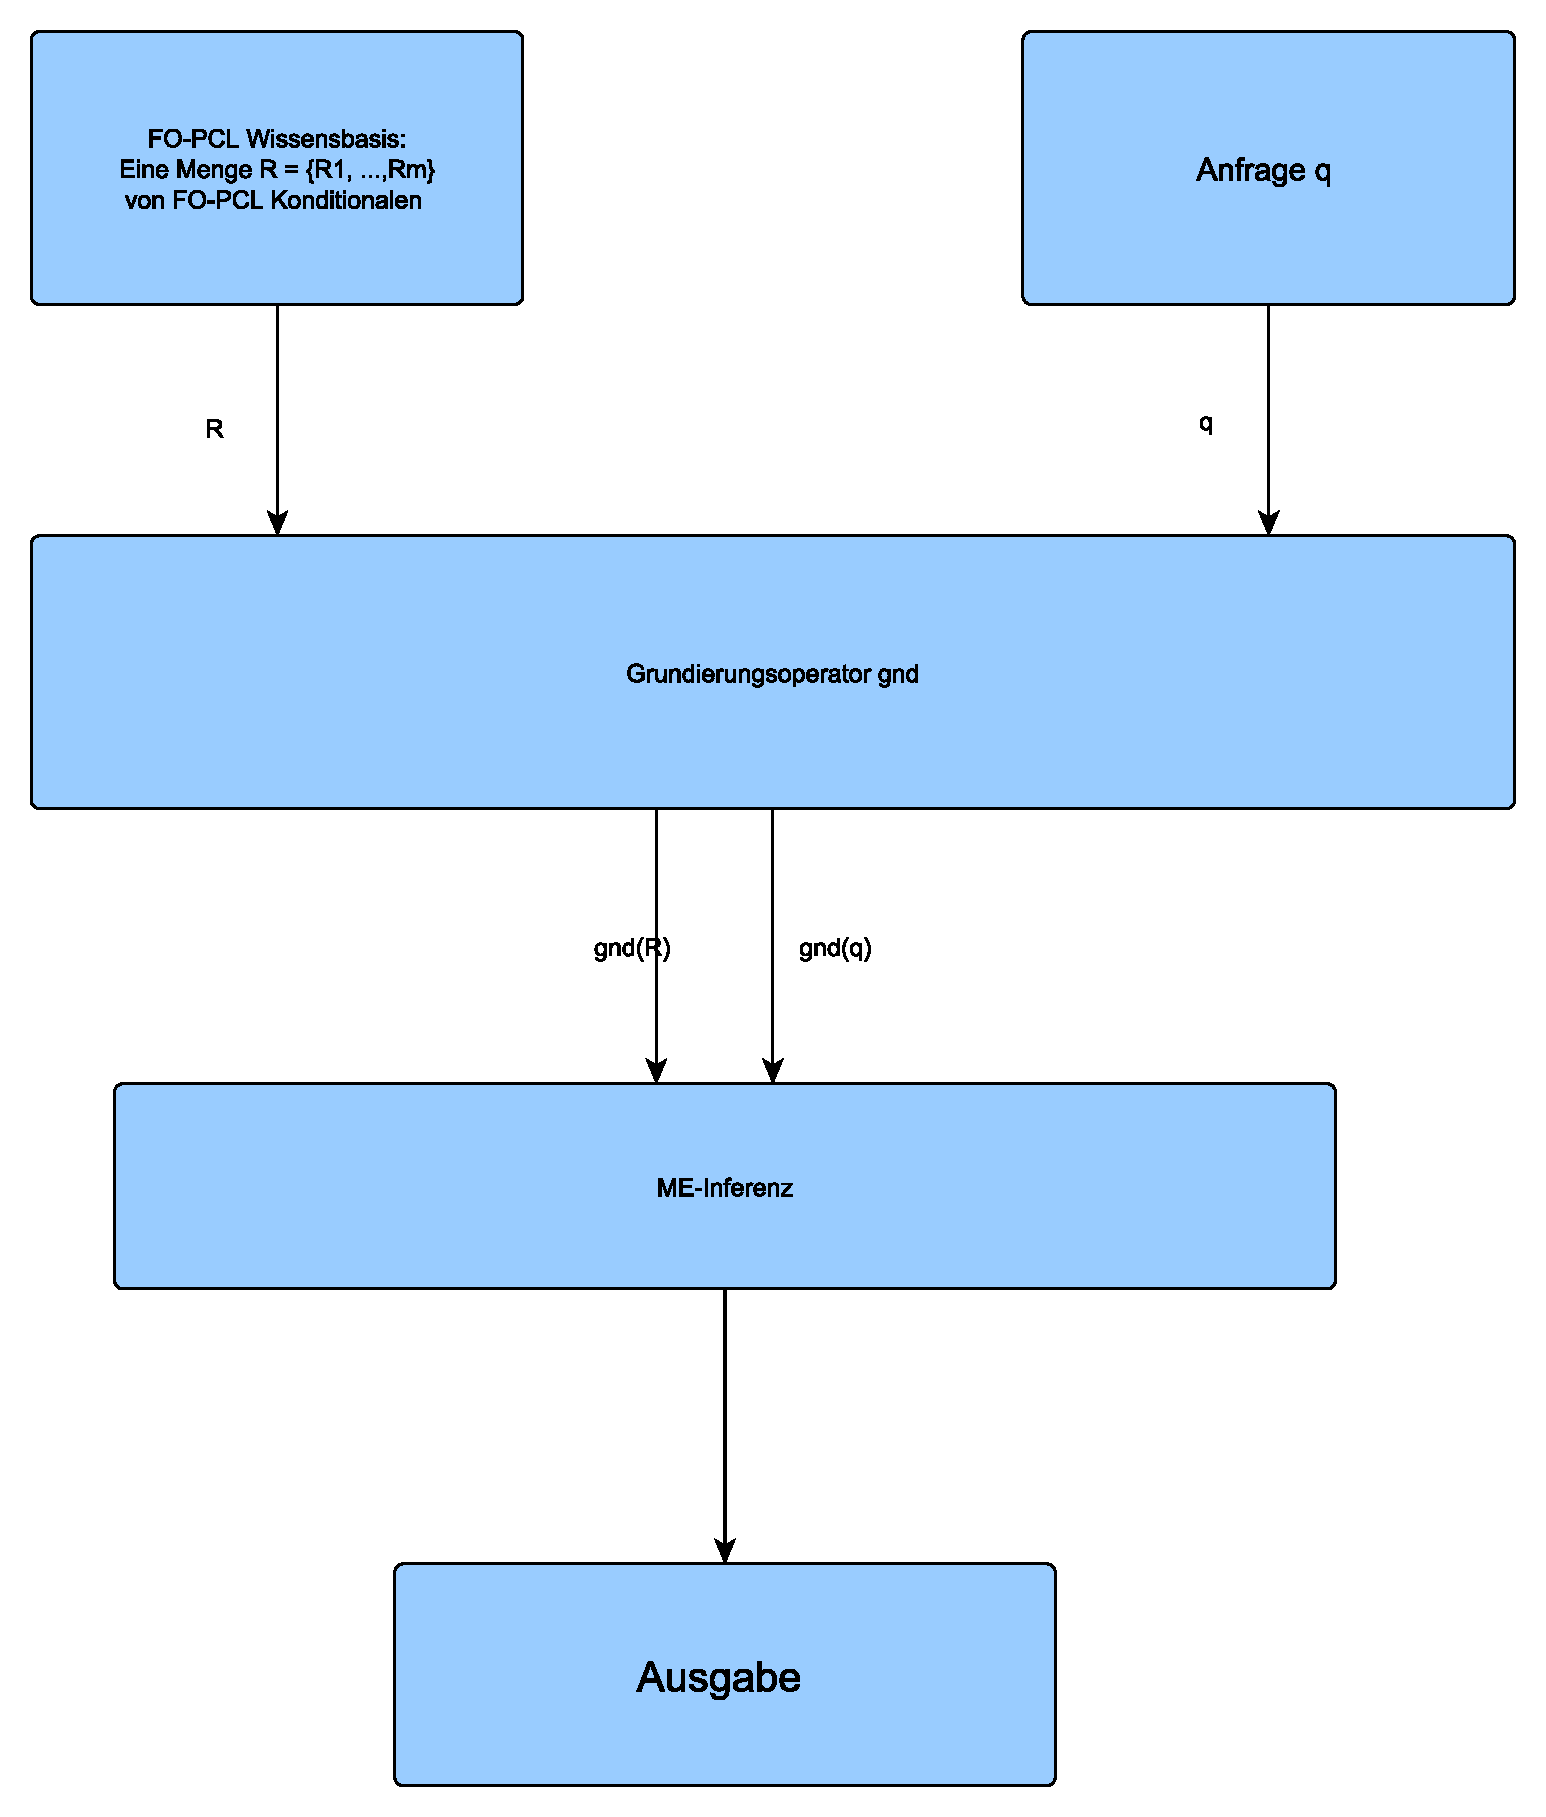
\includegraphics[scale = 0.5]{Graphics/FO-PCL_Inferenzprozess}
\begin{figure}[h]
	\caption{Der FO-PCL Inferenzprozess -allgemein- }\
\end{figure}
\\
Vergleiche auch \cite{BHM14}.

\section{Der Inferenzprozess der Komponente}
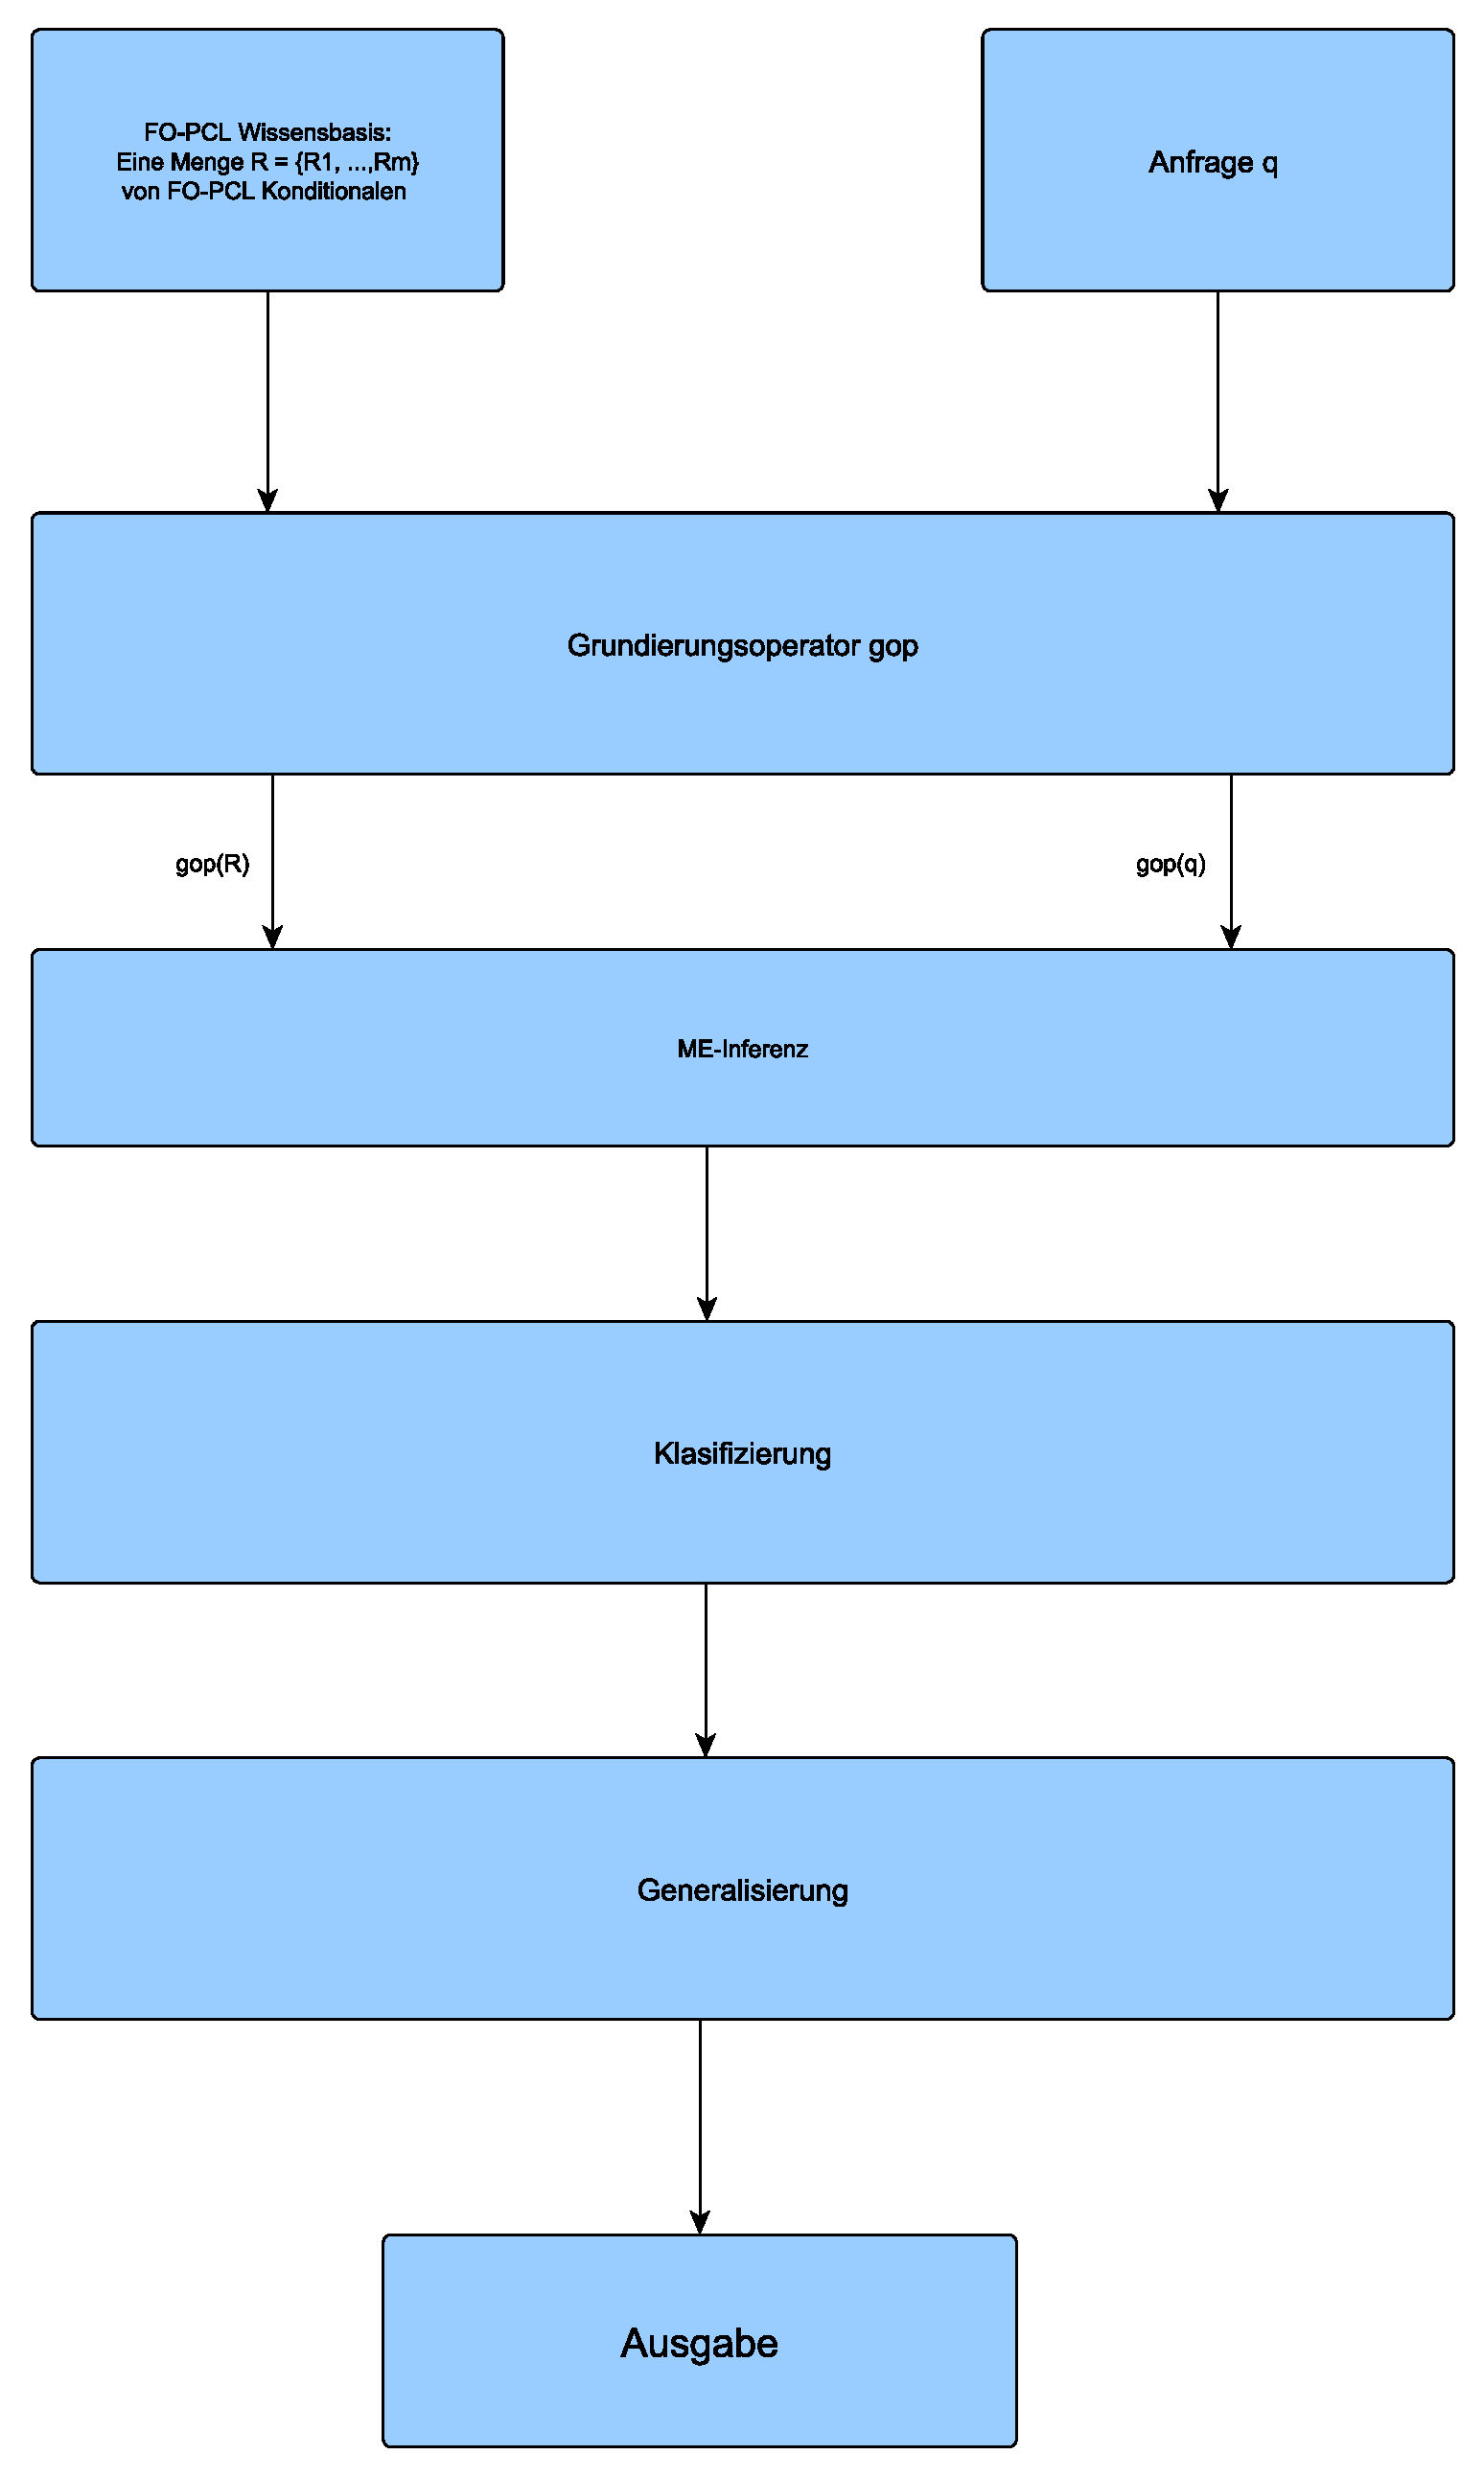
\includegraphics[scale = 0.4]{Graphics/Inferenzprozess_Komponente}
\begin{figure}[h]
	\caption{Der Inferenzprozess der Komponente }\
\end{figure}
\\
	
\subsubsection{Definition einer Wissensbasis}	
Um in FO-PCL Inferenz betreiben zu können, ist es zunächst notwendig, das erworbene bzw. vorhandene Wissen gemäß der Syntax in FO-PCL in einer Wissensbasis zu formulieren. Eine Wissensbasis ist Voraussetzung, um vorhandenes Wissen in eine Form zu bringen, in der es verarbeitet werden kann und ist notwendig, um mit der Inferenzkomponente Wissen ableiten zu können. Dazu wird eine Menge von Konditionalen definiert, die das vorhandene Wissen repräsentieren.  Diese Informationen über die Domäne inklusive der Abhängigkeiten und Wahrscheinlichkeiten müssen vom Benutzer zur Verfügung gestellt werden. Ob das bereitgestellte Wissen aus statistisch erhobenen Daten stammt oder Erfahrungswerte, möglicherweise sogar Schätzungen beinhaltet, ist dabei irrelevant.

\subsubsection{Überführung der relationalen Wissensbasis in eine propositionale Wissensbasis}
Es ist notwendig, die Wissensbasis zu grundieren indem die Konditionale unter Beachtung der Constraints grundiert werden. Dazu werden den Termen, soweit sie Variablen enthalten, Konstanten (aus der Domäne bzw. dem Universum)zugeordnet. Das geschieht gemäß der Semantik von FO-PL, vgl. \ref{sec:semantik}.
	
\subsubsection{Modellselektion}
Unter den Modellen, welche die Wissensbasis erfüllen, wird dasjenige Modell ausgewählt, das die Entropie maximiert. Dazu werden zunächst alle möglichen Welten berechnet. Danach wird die Welt mit der höchsten Entropie selektiert, vgl. \ref{Modellselektion}. Dabei erhält man einen epistemischen Zustand.
	
\subsubsection{Beliebige Anfragen}
Jetzt können beliebige Anfragen in Form eines unbedingten Konditionals gestellt werden.   

\subsubsection{Grundierung der Anfrage}

Das angefragte, unbedingte Konditional wird gemäß der Syntax von FO-PCL grundiert, d.h. es werden alle Grundkonditionale, vgl. Definition \ref{Fo-PCL Konditional}, für das angefragte Konditional durch Anwendung einer Grundsubstitution, vgl. Proposition \ref{Grundsubstitution} generiert.

\subsubsection{Berechnung der Wahrscheinlichkeit für jedes Grundkonditional}
Es wird zu jedem Grundkonditional eine Wahrscheinlichkeit mit Hilfe des epistemischen Zustands, der zur Wissensbasis gehört und der eine Wahrscheinlichkeitsfunktion umfasst, berechnet. Die Antwort zu diesem Zeitpunkt beinhaltet die Menge der Grundinstanzen des angefragten Konditionals und die jeweils dazu berechnete Wahrscheinlichkeit. Dabei wird von der berechneten Wahrscheinlichkeit erwartet, dass sie die Sicherheit angibt, mit der die Frage unter Berücksichtigung des bisher erworbenen Wissens beantwortet werden kann.
	
\subsubsection{Klassifizierung der Grundinstanzen} \index{Grundinstanz}
Die einzelnen Grundinstanzen des angefragten Konditionals, welche die gleichen Wahrscheinlichkeiten enthalten, werden in Klassen zusammengefasst.

\begin{Def}[Äquivalenzrelation] \label{Äquivalenzrelation}
Eine Äquivalenzrelation auf einer Menge $ \cal{R} $  ist eine Teilemenge $ \cal{M} \subset \cal{R} \times \cal{R}$, welche folgende Bedingungen erfüllt:\\
\begin{itemize}
	\item Reflexivität:\\
	 Für alle $ R \in \cal{R} $ ist $ (R,R) \in \cal{M} $.
	\item Symmetrie: \\
	Für alle $ U,V \in \cal{R} $ für, die auch  $ (U,V) \in \cal{M} $ gilt, ist auch  $ (V,U) \in \cal{M} $.
	\item  Transitivität:\\
	Für alle $ U,V,X  \in \cal{R} $ mit $ (U,V) \in \cal{M} $ und $ (V,X) \in \cal{M} $ ist auch $ (U,X) \in \cal{M} $.
\end{itemize}
\end{Def}



\begin{Def}[Parametrische Äquivalenz von FO-PCL Konditionalen] \label{Äquivalenz in FO-PCL} \index{Äquivalenz ! parametrische} \index{FO-PCL Konditional}
	Sei $  \cal{R} $ eine Menge von FO-PCL Konditionalen. Es gelte für alle $ R \in \cal{R} $, dass sie Grundinstanzen des gleichen Konditionals sind. Zwei Konditionale $ U,V \in \cal{R} $ sind parametrisch äquivalent, wenn sie den gleichen Parameterwert, d.h. die gleiche vorgegebene Wahrscheinlichkeit besitzen, sh. auch \ref{sec:parÄ}.\\
	Zwei FO-PCL Konditionale sind in der gleichen Äquivalenzklasse bezüglich der Äquivalenzrelation, wenn sie parametrisch äquivalent sind. \label{Äquivalenzklassen} \index{Äquivalenzklassen}
\end{Def}


\begin{Bsp}[Parametrische Äquivalenz von FO-PCL Konditionalen]\label{Bsp:parametische Äquivalenz}
	Für das Beispiel "{} Birds "{}, \ref{Birds} sind für die Anfrage $ (flies(X)) $ die Grundkonditionale $ (flies(Sylvester)), (flies(Bully)) $ und $ (flies(Kirby)) $ mit der Wahrscheinlichkeit von jeweils $ [0.664] $ parametrisch äquivalent.
\end{Bsp}	



Bei der Klassifizierung durch die Komponente sind in der praktischen Umsetzung die folgenden Dinge zu beachten. 
Da sich die Inferenzkomponente zur Berechnung der Wahrscheinlichkeit auf Komponenten aus Log4KR bedient, wird für nicht zulässige Anfragen das Ergebnis "{}-1"{} ermittelt. Unzulässige Anfragen können beispielsweise Anfragen sein, bei denen die Wahrscheinlichkeit der Prämisse des bedingten Konditionals Null ist.\\
Das Ergebnis  "{}0"{} erhält man unter anderem für reflexives Wissen, da dies durch den Algorithmus von Log4KR ausgeschlossen wurde wenn es zu einer inkonsistenten Wissensbasis führen würde, bzw. mit der Wahrscheinlichkeit  "{}0"{} belegt wurde. 
	
	
	
	
\subsubsection{Generalisierung der Klassen}
\textcolor{blue}{
	\begin{Def}[Qualitatives Konditional]\label{qualitatives_Konditional} \index{Konditional ! qualitatives}
		Sei $ \Sigma = (S, {\cal D}, Präd) $ eine mehrsortige Signatur und sei $ \cal{R}  $ eine FO-PCL Wissensbasis, gemäß Definition \ref{KB}.	
		Unter einem qualitativen Konditional im Sinne dieser Arbeit versteht man ein Konditional ohne zugeordnete Wahrscheinlichkeit, d.h. ein nicht quantifiziertes Konditional. \label{quantifiziertes_Konditional} \index{Konditional ! quantifiziertes}\\
		Dagegen ist unter einem quantifizierten Konditional ein Konditional mit zugeordneter Wahrscheinlichkeit zu verstehen.
	\end{Def}
}

	\begin{Bsp}[Qualitatives Konditional] \label{Bsp:Qualitatives Konditional}
		Für das Beispiel "{}Birds"{}, \ref{Bsp:Birds} sieht ein qualitatives Konditional so aus: \\
		$(flies(Tweety))$ oder auch $(flies(X))$\\
		Ein quantifiziertes Konditional dagegen sieht so aus:\\
		$(flies(Tweety))[0.0]$, $ (flies(X)[0.664]) $\\ 
	\end{Bsp}


\textcolor{blue}{
\begin{Def}[Generalisierung, generalisiertes Konditional]\index{Generalisierung} \index{Konditional ! generalisiertes}\label{Generalisierung}
Sei $ \Sigma = (S, {\cal D}, Präd) $ eine mehrsortige Signatur und sei $ \cal{R}  $ eine FO-PCL Wissensbasis, gemäß Definition \ref{KB}. Sei ferner $ Q $ eine Anfrage in Form eines qualitativen Konditionals und sei  $ \cal{E}$  $ = \{E_1, ..., E_t\}$ eine Menge von Äquivalenzklassen von FO-PCL Konditionalen gemäß Definition \ref{Äquivalenzklassen}.\\
	Eine Generalisierung ist eine Abbildung, die jeder Äquivalenzklasse $ E_i \in \cal{E} $  $ mit$  $ i \in \{1, ..., t\} $ jeweils genau ein einziges quantifiziertes Konditional $R_{gen} $, d.h. ein Konditional mit der für das Modell berechneten Wahrscheinlichkeit der Äquivalenzklasse, zuordnet.  $R_{gen} $ wird im Folgenden auch generalisiertes Konditional genannt. \index{Konditional ! generalisiertes}  $R_{gen} $ muss der Signatur folgen und darf in Prämisse und Konklusion nur Variablen enthalten, wenn die Äquivalenzklasse mehr als ein Konditional enthält. Aus  $R_{gen} $ müssen jeweils alle Konditionale der zugehörigen Äquivalenzklasse mit den Konstanten in $ \cal{D} $ und unter Beachtung des Constraints durch Grundsubstitution, vgl. \ref{Grundsubstitution} gebildet werden können. Für Äquivalenzklassen mit einem Konditional entspricht  $R_{gen} $ genau diesem Konditional.  Bei $R_{gen} $ handelt es sich für diesen Fall folglich um ein Grundkonditional mit zugeordneter Wahrscheinlichkeit. 	
\end{Def}
D.h. in der Phase der Generalisierung werden die Konditionale, die sich aufgrund der gleichen Wahrscheinlichkeit in einer Äquivalenzklasse befinden, zu einem möglichst allgemeinen Konditional zusammengefasst.\\
Die eigentliche Leistung der Komponente liegt hierbei in der Erzeugung des jeweiligen Konditionals. Wie das Konditional der Klasse aussieht, hängt von der Klasse und dem ausgeführten Generalisierungsprozess ab. 
\begin{Bsp}[Generalisierung]\label{Bsp:Generalisierung}
Für das Beispiel "{} Birds "{}, \ref{Birds} könnten für die Anfrage $ (flies(X)) $ bei einer möglichen Generalisierung der beiden Klassen folgende generalisierten Konditionale ergeben: \\
\\
\noindent
Sei nun $ \cal{R} $$_{Birds}  $ = $ (T_1, T_2, T_3)  $ die FO-PCL Wissensbasis aus dem Beispiel mit den Konditionalen
\\
$ T_{1} : \langle (flies(X) \mid isBird(X)[0,9], X \neq Tweety \rangle$\\	
$ T_{2}  :  \langle (flies(Tweety))[0], \top \rangle $,\\
$ T_{3} : \langle (isBird(Tweety) [1], \top \rangle$\\
\\
Äquivalenzklasse 1: $\{(flies(Tweety))[0.0]\}$\\
Äquivalenzklasse 2: $\{(flies(Bully))[0.664], (flies(Sylvester))[0.664], (flies(Kirby))[0.664]\}$\\
\noindent
Generalisiertes Konditional für Äquivalenzklasse 1: $\{(flies(Tweety))[0.0]\}$\\
Generalisiertes Konditional für Äquivalenzklasse 2: $\{(flies(X))[0.664]<X \neq Tweety>\}$\\
\\
Wie man unschwer erkennen kann, entspricht das generalisierte Konditional der Äquivalenzklasse dem (einzigen) Konditional, das sich in der Äquivalenzklasse 1 befindet.\\
Aus dem generalisierten Konditional für die Äquivalenzklasse 2 lassen sich durch Grundsubstitution genau die Konditionale der Äquivalenzklasse bilden.
\end{Bsp}
}

\textcolor{blue}{
\subsubsection{Ausgabe der Komponente}
\begin{Def}[Ausgabe der Komponente] \index{Ausgabe der Komponente} \label{Ausgabe der Komponente}
	Sei $ \Sigma = (S, {\cal D}, Präd) $ eine mehrsortige Signatur und sei $ \cal{R}  $ eine FO-PCL  Wissensbasis, gemäß Definition \ref{KB}. Sei ferner  $ \cal{Q} $ eine nichtleere Menge von Anfragen in Form qualitativer Konditionale und sei $ G $ die Menge aller generalisierter Konditionale, vgl. \ref{Generalisierung}, d.h. die Konditionale die der Signatur $ \Sigma $ folgen und die aus der Wissensbasis durch den Inferenzprozess über Grundierung, ME-Inferenz, Klassifizierung und Generalisierung, gebildet werden können.\\
	Die Ausgabe der Komponente zu einer Anfrage ist eine nichtleere Menge von generalisierten Konditionalen gemäß o.g. Definition. 
	\end{Def}
\begin{Bsp}[Ausgabe der Komponente] \label{Bsp:Ausgabe der Komponente}
Für das Beispiel "{} Birds "{}, \ref{Birds} ist für die Anfrage $ (flies(X)) $ die Ausgabe der Komponente: \\
\noindent
$ \{(flies(Tweety))[0.0], (flies(X))[0.66] <X \neq Tweety>\}$
\end{Bsp}
}


	
\chapter{Experimentelle Forschungen} \label{Experim. Forschungen}
Als Ausgangsbasis für die Erstellung eines Algorithmus wurden verschiedene Beispiele betrachtet. Der Großteil der Beispiele ist der Bibliothek Log4KR entnommen. Es wurden verschiedene Anfragen an die Wissensbasis gestellt, um ermitteln zu können, welche Ergebnisse die Anfragen liefern. Das diente dazu Vermutungen zu bestätigen bzw. erste Erkenntnisse zu erhalten.\\
Unzulässige Anfragen sollten nicht an die Wissensbasis gestellt werden. Das sind solche, deren Prämisse die Wahrscheinlichkeit Null besitzt und die sonst zu einer Division durch Null führen würde.\\
Eine detaillierte Beschreibung der Beispiele in Fo-PCL Syntax, aufbereitet zur Verarbeitung in Log4KR findet sich im Anhang \ref{examples}.


Bei den Beispielen findet sich der Begriff "{}angestrebte Ausgabe"{}.\index{angestrebte Ausgabe}\\
\textbf{Angestrebte Ausgabe}\\
\label{angestrebte Ausgabe}
\emph{Unter der angestrebten Ausgabe im Sinne dieser Arbeit ist das Ergebnis eines Prozesses der Betrachtung und des Vergleichs der Klassen zu verstehen. Dieser Prozess endet mit der Generierung eines möglichst allgemeinen Konditionals. Die angestrebten Ausgabe ist somit das Resultat einer manuellen Betrachtung. Dabei ist es das Ziel, dass der Constraint jedes erzeugten Konditionals möglichst kurz ist, d.h., er soll möglichst wenig Junktoren und Terme enthalten. Es soll im Wege des Inferenzprozesses eine Menge von Konditionalen erzeugt werden, die identisch oder zumindest logisch äquivalent (im Sinne boolescher Algebra) mit der angestrebten Ausgabe sind.  Die generierten Konditionale sollten dabei intersubjektiv als möglichst allgemein akzeptiert werden.\\
Ob das algorithmisch so umsetzbar ist, werden die weiteren Forschungen ergeben.}

\section{Annahmen}

\begin{itemize}
	\item Generische Grundkonditionale habe die gleiche Wahrscheinlichkeit
	\item Spezifisches Wissen führt zu unterschiedlichen Wahrscheinlichkeiten
	\item Die Belegung verschiedener Variablen mit gleichen Konstanten hat Einfluss auf die Wahrscheinlichkeiten (und damit auf die Anzahl der Klassen)
	
\end{itemize}


\fontsize{11pt}{13.2pt}\selectfont

\setlongtables


\setlength{\currentLongTableWidth}{\textwidth} %setze neue länge auf textbreite
\addtolength{\currentLongTableWidth}{-4\tabcolsep} %subtrahiere -8\cdot textbreite von asdf, 2 Abstände pro Zelle * Anzahl der Spalte
\begin{footnotesize}
	\begin{longtable}{| >{\raggedright} p {0.15\currentLongTableWidth} | p {0.15\currentLongTableWidth} |>{\raggedright} p {0.15\currentLongTableWidth} | p {0.15\currentLongTableWidth} | p {0.15\currentLongTableWidth} | p {0.15\currentLongTableWidth} |}
		\hline
		\multicolumn{6}{|c|}{\textbf{Beispiele}}\\\hline\hline
			\hline
			\textbf{Prädikate} 
			& \textbf{ohne spezifische Konstante} 
			& \textbf{spezifische Konstante} 
			& \textbf{transitives Wissen} 
			& \textbf{transitives Wissen und spezifische Konstante}
			& \textbf{zwei Sorten}\\
		\endhead
		\hline
		\endfoot
		\endlastfoot
			\hline
				\textbf{einstellig} 
					& BirdsEqual \ref{BirdsEqual}
					& Birds \ref{Birds}, \newline Birds2Birds \ref{Birds2Birds}, \newline	Birds2Classes \ref{Birds2Classes}, \newline BirdsNot \ref{BirdsNot}, \newline Birds\-With\-out\-Null \ref{BirdsWihoutNull}, \newline BirdsDiffer \ref{BirdsDiffer}
					&
					&
					&\\
					
			\hline
				\textbf{zweistellig}
					& Cold \ref{Cold}, \newline Sport \ref{Sport}, \newline Friendship \ref{Friendship}, \newline MonkeysA \ref{MonkeysA}-
					& Misanthrope \ref{Misanthrope}, \newline Mis\-an\-thro\-pe\-3\-Clas\-ses, \newline SportEx \ref{SportEx}, \newline  Mis\-an\-thro\-pe\-Ir\-re\-flex\-ive \ref{MisanthropeIrreflexive}, \newline Monkeys2 \ref{Monkeys2},\newline SportExN \ref{SportExN}
					& Friendship \ref{Friendship} 
					& Friend\-ship\-With\-Mis\-an\-thro\-pe \ref{FriendshipWithMisanthrope}
					& Garfield \ref{Garfield} \\
			\hline
				\textbf{ein- und zweistellig} 
					& SportExNFam \ref{SportExNFam}, \newline Cold\-Spez \ref{ColdSpez}
					& ColdTrans \ref{ColdTrans} 
					& ColdTrans\-Spez \ref{ColdTransSpez}
					&
					&\\
			 \hline
		\caption{Übersicht über die Beispiele}
	\end{longtable}
\end{footnotesize}




\section{Einstelliges Prädikat}
\begin{itemize}


\item{Spezifische Konstante und zwei spezifische Fakten}
Hier wurden verschiedene Konstellationen und Anfragen getestet um auswertbares Material zu erhalten.
\begin{itemize}
	\item \textsl{Birds} \label{BBirds} s. \ref{Birds}: \\
	Das klassische Beispiel der Konditionallogik. In der Aufgabenstellung als Minimalbeispiel erläutert. Das spezifische Wissen über Tweety (spezifische Konstante) führt bei allen hier gestellten Anfragen, dazu, dass die spezifischen Grundinstanzen, in denen Tweety vorkommt eine andere Wahrscheinlichkeit haben als die generischen Grundinstanzen, die wiederum alle die gleiche Wahrscheinlichkeit in den gestellten Anfragen haben.
	
	\item \textsl{Birds2Birds} \label{BBirds2Birds} s. \ref{Birds2Birds}:\\
	Das ist die Minimalvariante zu Birds. Dieses Beispiel wurde genutzt, um die gesamte Wahrscheinlichkeitsverteilung zu betrachten und zu ermitteln ob die Wahrscheinlichkeiten sich zu 1 addieren. Es diente der Überprüfung der Korrektheit des Optimierungsprozesses der Bibliotheksfunktion aus Log4KR. Für dieses Beispiel addieren sich die Wahrscheinlichkeiten zu 1 und die Ungenauigkeiten zwischen den Wahrscheinlichkeiten der einzelnen Grundinstanzen ergeben sich offensichtlich aus der eingestellten Ungenauigkeit.
	
	\item \textsl{Birds2Classes} \label{BBirds2Classes} s. \ref{Birds2Classes}:\\
	Das Birds Beispiel mit weniger Konstanten, spezifischem Wissen und zwei Klassen. Erwartungsgemäß haben die generischen Grundinstanzen die gleiche Wahrscheinlichkeit und die spezifische eine andere.
	
	\item \textsl{BirdNot} (Beispiel Birds um negierte Anfragen erweitert) \label{BBirdsNot} s. \ref{BirdsNot}
	
	\item \textsl{BirdsWithoutNull} (enthält kein spezifisches Wissen mit Wahrscheinlichkeit Null) \label{BBirdsWithoutNull} s. \ref{BirdsWihoutNull}
	Das Birds Beispiel mit negierten Anfragen. Auch das ändert nichts daran, dass die spezifischen Grundinstanzen eine andere Wahrscheinlichkeit als die generischen haben und die generischen die gleiche Wahrscheinlichkeit.
	
\end{itemize}

\item{Spezifische Konstanten und spezifische Fakten}
\begin{itemize}
	\item \textsl{Birds3Classes} \label{BBirds3Classes} s. \ref{Birds3Classes}:\\
	Das Birds Beispiel mit zwei spezifischen Konstanten, spezifischem Wissen und drei Klassen. Erwartungsgemäß haben die generischen Grundinstanzen die gleiche Wahrscheinlichkeit und die spezifischen jeweils eine andere.
	
\end{itemize}

\item{Ausschließlich spezifische Konstanten und spezifische Fakten}
\begin{itemize}
	\item \textsl{BirdsDiffer} \label{BBirdsDiffer} s. \ref{BirdsDiffer}:\\

	Hier ist jede Konstante eine spezifische Konstante. Und für jede hier gestellte Anfrage ergeben sich für jede Grundinstanz und jede spezifische Konstante unterschiedliche Wahrscheinlichkeiten mit Ausnahme der Anfrage, die spezifisches Wissen über Tweety in der Konklusion enthält. Die Konklusion enthält für die anderen spezifischen Konstanten keine spezifische Information. Es sind die Grundinstanzen trotz spezifischer Prämisse für jede Konstante im Übrigen gleich, das heißt hier führt nur eine spezifische Konstante zur Unterscheidung. Für diese gilt das spezifische Grundkonditional der Konklusion wurde bereits in der Wissensbasis mit der Wahrscheinlichkeit von Null definiert. 

\end{itemize}

\item{Keine spezifischen Fakten oder Konstanten}
\begin{itemize}
	\item \textsl{BirdsEqual} \label{BBirdsEqual} s. \ref{BirdsEqual}:\\

	Alle (generischen) Grundinstanzen besitzen die gleiche Wahrscheinlichkeit.
\end{itemize}
\end{itemize}

\section{Zweistelliges Prädikat}
\begin{itemize}
\item {Keine spezifischen Konstanten}
\begin{itemize}
	\item \textsl{Cold} \label{BCold} s. \ref{Cold}:\\

	Das Beispiel aus der Literatur. Mit Ausnahme des reflexiven Wissens, das nicht ausgeschlossen wurde in der Wissensbasis sind erwartungsgemäß alle Grundinstanzen des jeweils angefragten Konditionals gleich.

	\item \textsl{Sport} \label{BSport} s. \ref{Sport}:\\
	
	Ein Minimalbeispiel mit einem Konditional. Alle generischen Grundinstanzen des jeweils angefragten Konditionals sind gleich.

	
\end{itemize}

\item{Keine spezifischen Konstanten und eine Konjunktion mit transitivem Wissen als Prämisse}
\begin{itemize}
	\item \textsl{Friendship} \label{BFriendship} s. \ref{Friendship}:\\

	Bei den angefragten Konditionalen, die in Prämisse oder Konklusion reflexives Wissen enthielten, welches in der Wissensbasis ausgeschlossen wurde, wurde die Wahrscheinlichkeit zu Null berechnet. Im Übrigen hatten die generischen Grundinstanzen die gleiche Wahrscheinlichkeit. Die Transitivität hat keinen Einfluss auf das Ergebnis.
\end{itemize}

\item{Eine spezifische Konstante und eine Konjunktion mit transitivem Wissen als Prämisse}
\begin{itemize}
	\item \textsl{FriendshipWithMisanthrope} \label{BFriendshipWithMisanthrope} s. \ref{FriendshipWithMisanthrope}:\\
	Das reflexive Wissen wurde in der Wissensbasis ausgeschlossen und daher zu Null berechnet. Generische Grundinstanzen haben die gleiche Wahrscheinlichkeit. Die spezifischen jeweils auch. Das transitive Wissen macht keinen Unterschied.

\end{itemize}

\item{Eine spezifische Konstante}
\begin{itemize}
	\item \textsl{Misanthrope} \label{BMisanthrope} s. \ref{Misanthrope}:\\
	Das reflexive Wissen wurde in der Wissensbasis ausgeschlossen und wird daher mit der Wahrscheinlichkeit Null berechnet. Generische Grundinstanzen haben die gleiche Wahrscheinlichkeit. Die spezifischen jeweils auch. 
	\item \textsl{SportEx} \label{BSportEx} s. \ref{SportEx}:\\
	Generische Grundinstanzen haben die gleiche Wahrscheinlichkeit. Die spezifischen jeweils auch. 

\end{itemize}

\item{Eine spezifische Konstante und das reflexive Wissen ist mit der Wahrscheinlichkeit von Null vorbelegt}
\begin{itemize}
	\item \textsl{MisanthropeIrreflexive} \label{BMisanthropeIrreflexive} s. \ref{MisanthropeIrreflexive}:\\
	Das Ergebnis ist das gleiche wie beim Beispiel Misanthrope. Insgesamt ist aber die Vorbelegung des reflexiven Wissens mit einer Wahrscheinlichkeit von Null in diesem Fall sinnvoll, um unsinnige Ergebnisse oder philosophische Grundfragen zum Thema Selbstliebe zu vermeiden. Die Frage mit welcher Wahrscheinlichkeit sich jemand selbst liebt und was dabei ein zu erwartendes Ergebnis wäre,  wird somit nicht zur Diskussion gestellt.

\end{itemize}

\item{Eine spezifische Konstante, ein spezifisches Konditional und verschiedene andere Konditionale}
\begin{itemize}
	\item \textsl{Monkeys2} \label{BMonkeys} s. \ref{Monkeys2}:\\
	Die spezifische Konstante führt je nach Vorkommen, also in der Prämisse oder Konklusion und dort jeweils in der Teilformel zu einer anderen Wahrscheinlichkeit und damit zu einer anderen Klasse. Alle generischen Grundinstanzen beinhalten die spezifische Konstante in irgendeiner Form. Die generischen Grundinstanzen haben unterschiedliche Wahrscheinlichkeiten
	\item \textsl{SportExN} \label{BSportExN} s. \ref{SportExN}:\\
	Die spezifische Konstante führt zu spezifischen Grundinstanzen. Generische Grundinstanzen haben erwartungsgemäß die gleiche Wahrscheinlichkeit. Für jede Anfrage an die Wissensbasis gilt, dass die generischen Grundkonditionale die gleiche Wahrscheinlichkeit haben. Bei allen generierten Konditionalen ergeben sich die gleichen Constraints.
	
\end{itemize}

\item{Keine spezifische Konstante und zwei Konditionale}
\begin{itemize}
	\item \textsl{MonkeysA} \label{BMonkeysA} s. \ref{MonkeysA}:\\
	Alle nicht reflexiven Grundinstanzen haben die gleiche Wahrscheinlichkeit. Die reflexiven Grundinstanzen sind in der Wissensbasis ausgeschlossen und deren Wahrscheinlichkeit wird daher mit Null berechnet.

\end{itemize}
	
\item{Zwei Sorten, eine spezifische Konstante, verschiedene Konditionale}
\begin{itemize}
	\item \textsl{Garfield} \label{BGarfield} s. \ref{Garfield}:\\
	Generische Grundinstanzen haben die gleiche Wahrscheinlichkeit. Spezifische Konstanten führen zu unterschiedlichen Wahrscheinlichkeiten.
\end{itemize}

\item Zwei spezifische Konstanten 
\begin{itemize}
 \item{Misanthrope2Spez}	\label{BMisanthrope2Spez} s. \ref{Misanthrope2Spez}:\\
Log4KR kann dieses Beispiel nicht berechnen. Weitere Forschungen für die Verwendung von mehr als zwei spezifischen Konstanten können daher nicht unternommen werden.
\end{itemize}


	\item Drei spezifische Konstanten 
	\begin{itemize}
		\item{Misanthrope3Spez}	\label{BMisanthrope3Spez} s. \ref{Misanthrope3Spez}:\\
	Log4KR kann dieses Beispiel nicht berechnen. Weitere Forschungen für die Verwendung von mehr als zwei spezifischen Konstanten können daher nicht unternommen werden.
	\end{itemize}

\end{itemize}
\section{Ein- und zweistellige Prädikate}
\begin{itemize}
\item{Ein- und zweistellige Prädikate, eine spezifische Konstante und verschiedene Konditionale mit spezifischem Wissen}
\begin{itemize}
	\item \textsl{SportExNFam} \label{BSportExNFam} s. \ref{SportExNFam}:\\
	Dieses Beispiel dient der Erweiterung des Beispiels "{}SportExN"{} (s. \ref{SportExN}) um ein zweistelliges Prädikat. Alle generischen Grundkonditionale sind für die jeweilige Anfrage gleich. Das Vorkommen der spezifischen Konstante führt in fast allen Anfragen zusammen mit der Betrachtung des reflexiven Wissens zu unterschiedlichen Wahrscheinlichkeiten und zu den gleichen Constraints für die jeweilige Klasse.\\
	In der Anfrage $\langle (normalWeight(X) \mid (sport(X) \land family(X,Y)) \rangle$\\ führt alleine die spezifische Konstante unabhängig vom reflexiven Wissen zur Unterscheidung. Das ergibt sich daraus, dass die Wahrscheinlichkeit der in der Prämisse vorkommenden Terme in diesem Fall gleich sind. $(sport(Chris)) $ hat per Definition in der Wissensbasis die gleiche Wahrscheinlichkeit wie $family(X,X)$.
	\item \textsl{ColdSpez} \label{BColdSpez} \ref{ColdSpez}:\\
Dieses Beispiel entspricht dem Beispiel "{}Cold"{}, s. \ref{Cold}, erweitert um spezifisches Wissen über eine Konstante des Universums. Für alle Anfragen haben die generischen Grundkonditionale die gleiche Wahrscheinlichkeit. Reflexives Wissen, welches in der Wissensbasis ausgeschlossen wurde, führt immer zu einer Unterscheidung. Im Übrigen führt nur die spezifische Konstante zur Unterscheidung.
\end{itemize}


\item{Ein- und zweistellige Prädikate, verschiedene Konditionale und transitives Wissen}
\begin{itemize}
	\item \textsl{ColdTrans} \label{BColdTrans} s. \ref{ColdTrans}:\\
Das Beispiel "{}Cold"{} erweitert um transitives Wissen. Unterschiedliche Wahrscheinlichkeiten ergeben sich durch die gleiche Belegung von Variablen, wobei diese Fälle in der Wissensbasis mit der Wahrscheinlichkeit von Null definiert wurden. Wenn die Prämisse eine Formel enthält, die in der Konklusion vorkommt und man diese Formel als wahr annimmt, so ist natürlich auch die Konklusion wahr und die Wahrscheinlichkeit erwartungsgemäß 100 \%.

 Man betrachte das unbedingte Konditional $\langle (cold(X) \mid ((contact(X,Y)  \land contact(Y,Z)) \land cold(Z)),  X = Z \rangle$ . Sei cold(Z) (als Teil der Prämisse) wahr. Dann ist $ cold(X) $ (also die Konklusion) auch wahr für X = Z, was nicht weiter überraschend ist, aber an dieser Stelle für erwähnenswert gehalten wurde, da es durchaus für den Entwurf eines regelbasierten Algorithmus relevant sein könnte. Das bedingte Konditional sollte damit wie folgt aussehen: $\langle (cold(X) \mid ((contact(X,Y)  \land contact(Y,Z)) \land cold(Z)) [1.00000],  X = Z \rangle$.\\ Im Ergebnis bleibt zu sagen, dass auch Transitivität zu keinen überraschenden Ergebnissen führt. Lediglich die Belegung unterschiedlicher Variablen mit gleichen Konstanten hat einen erheblichen Einfluss. Ebenso die Gestalt bzw. das Wissen der Anfrage.
\end{itemize}


\item{Ein- und zweistellige Prädikate, eine spezifische Konstante und verschiedene Konditionale und transitivem und spezifischem Wissen}
\begin{itemize}
\item \textsl{ColdTransSpez} \label{BColdTransSpez} s. \ref{ColdTransSpez}:\\
Dieses Beispiel ist die Erweiterung des Beispiels "{}ColdTrans"{} um spezifisches Wissen. Auch hier werden die bisherigen Ergebnisse bestätigt. Neben der Belegung unterschiedlicher Variablen mit gleichen Konstanten hat auch das spezifische Wissen der Wissensbasis einen Einfluss und führt zu mehr Klassen. Leider gibt es keine sofort erkennbaren einfachen Regeln, die der Aussagenlogik genügen. Was intuitiv logisch erscheint ist nicht unbedingt in dieser Form axiomatisierbar. Die Kombination von spezifischem, reflexiven und transitivem Wissen führt bei etwas komplexeren Anfragen zu einem zwar allgemeinen Konditional, aber sehr unübersichtlichen Constraint, s. die Anfrage $ (cold(Z)|(contact(X,Y) * contact(Y,Z) * cold(X))) $ führt könnte zur Ausgabe $ (cold(Z)|(contact(X,Y) * contact(Y,Z) * cold(X)))[1.0]<((((X != Y) * X = Z) * Y = anna) + ( X = Y * X = Z)) + (X = Z * Z = anna) * X != Y)) + (( X != anna * Y != anna * Z != anna))> $ für eine bestimmte Klasse führen. Ob sich das letzte Konditional in mehrere Konditionale (mit gleicher Wahrscheinlichkeit) aufteilen ließe, bleibt Aufgabe weiterer Nachforschungen, dürfte aber nicht trivial sein. 
\end{itemize}

\end{itemize}

\section{Beobachtungen}

	\begin{itemize}
		\item 	Generische Grundinstanzen \index{Grundinstanz ! generisch} sind unabhängig von der Wissensbasis und der gestellten Anfrage gleich.
		\item Die Verwendung spezifischer Konstanten  \index{Konstante ! spezifisch} führen in der Regel zu anderen Wahrscheinlichkeiten als die Verwendung nicht spezifischer Konstanten.
			\item Wenn mehrere spezifische Konstanten verwendet wurden, würde man erwarten, dass es eine Klasse gibt für jede spezifische Konstante, eine Klasse für reflexives Wissen und mehrere Klassen mit Kombinationen aus spezifischen Konstanten. Das ist nicht der Fall, wie man dem Beispiel \ref{Misanthrope2Spez} entnehmen kann.
		\item Wenn eine spezifische Konstante in einer Formel verwendet wurde, die in der Konklusion vorkommt, dann führt das zu einer anderen Wahrscheinlichkeit, unabhängig davon, ob auch die anderen Konditionale spezifisches Wissen enthalten. Die anderen Grundinstanzen haben die gleiche Wahrscheinlichkeit s. \ref{BirdsDiffer} für die Anfrage $ (flies(X) \mid isBird(X)$. Das hängt in diesem Fall daran, dass die Annahme der Prämisse einen Fakt enthält ($ flies(Tweety)[0] $) , wo die Wissensbasis im Übrigen nur unsicheres Wissen enthält. (Die Annahme der Anfrage ist, dass die Prämisse $isBird(X)$ ein Fakt ist (also zu $ 100\% $ gelte). In der Wissensbasis wird aber ausgesagt, dass $isBird(X)$ nur möglicherweise gilt.
		\item Enthält die Prämisse der Anfrage einen Fakt, der auch in der Konklusion vorkommt, so ist auch die Konklusion sicher (vgl. \ref{ColdTrans}:$(cold(carl) \mid ((contact(carl,anna)  \land cold(carl)) $). 
		\item Unterschiedliche Wahrscheinlichkeiten können sich aus den verschiedensten Gründen ergeben
		\item Unterschiedliche Wahrscheinlichkeiten ergeben sich bei spezifischem Wissen über (eine) bestimmte Konstante des Universums, vgl. \ref{Birds} beispielsweise für die Anfrage $ flies(X) $, wo sich für die spezifische Instanz des Konditionals eine andere Wahrscheinlichkeit als für die generischen ergibt (die ja die gleiche Wahrscheinlichkeit besitzen): $ flies(Tweety)[0.0] $ und $ flies(X)[0.663]<X \neq Tweety> $
		\item Unterschiedliche Wahrscheinlichkeiten ergeben sich auch, wenn kein spezifisches Wissen über bestimmte Konstanten in der Wissensbasis, sondern Variablen mit den gleichen Wahrscheinlichkeiten belegt werden, s.  im Beispiel "{}Cold"{} s. \ref{Cold} für die Anfrage $ contact(X,Y) $.
		\item Spezifisches Wissen und die Belegung unterschiedlicher Variablen mit gleichen Konstanten stehen in Interaktion.
		\item Bei zweistelligen Prädikaten führt die Belegung unterschiedlicher Variablen mit gleichen Konstanten immer zu einer gleichen Klasse, in der sich die Terme der Konditionale nur durch Umbenennung unterscheiden. Zum Beispiel führt die Anfrage $ contact(X,Y) $ im Beispiel "{}Cold"{} s. \ref{Cold} für reflexives Wissen zu der Klasse $ contact(anna,anna)[0.0], contact(bob,bo)[0.0] , contact(carl,carl)[0.0]  $.
		\item Interaktionen sind nicht trivial und nicht auf den ersten Blick erkennbar. Deutlich wird das am Beispiel "{}ColdSpez"{}, s. \ref{ColdSpez} bereits bei der trivialen Anfrage $ contact(X,Y) $, wo das spezifische Wissen über eine Konstante (hier: anna) mit dem reflexiven Wissen (also der Belegung unterschiedlicher Variablen mit den gleichen Konstanten des Universums) zu Interaktionen führt. Ähnliches gilt beim Beispiel "{}BirdsWithoutNull"{} für die Anfrage $ (flies(X) | isBird(X) $, wo das spezifische Wissen über Tweety nicht zu einer anderen Wahrscheinlichkeit führt als bei den generischen Instanzen. Das lässt sich allerdings einfach aus der Struktur der Anfrage erklären, da die Wissensbasis mit $ isBird(Tweety)[1.0] $ einen Fakt enthält, der die Prämisse erfüllt. Es wird daran deutlich, dass auch der Inhalt der Wissensbasis die Anzahl der Klassen beeinflussen kann, das aber wiederum in Abhängigkeit der Gestalt der Anfrage. Besonders kompliziert wird beispielsweise die (komplexe) Anfrage $ cold(Z)|contact(X,Y) * cold(X)) $ im Beispiel "{}ColdTransSpez"{}, s. \ref{ColdTransSpez}, bei der die Kombination aus spezifischem und reflexiven Wissen zu vielen Klassen führt.
		\item Die Anzahl der Sorten scheint auf den ersten Blick keinen Unterschied für die Anzahl der Klassen zu machen; wesentlicher ist das Vorhandensein von spezifischen Konstanten gleich welcher Sorte. Daher wird darauf kein weiterer Fokus gesetzt. Allerdings wird der generierte Constraint komplexer, s. Anfrage $ (isStupid(Y)|moreIntelligent(X,Y)) $ im Beispiel "{}Garfield"{}, \ref{Garfield}
		\item Die Komplexität der Anfrage hat einen Einfluss darauf, wie viele Klassen gebildet werden bzw. auf die Komplexität des Constraints. 	
 
	\end{itemize}


	\section{Fazit}
		\begin{itemize}
	\item Unterschiedliche Wahrscheinlichkeiten resultieren aus
	\begin{itemize}
		\item der Verwendung spezifischer Konstanten \index{Konstante ! spezifisch}
		\item der Belegung von Variablen mit den gleichen Konstanten
		\item sicherem Wissen in der Anfrage
		\item der Wechselwirkung zwischen dem Wissen der Anfrage und dem Wissen der Wissensbasis
		\item der Wechselwirkung von spezifischem Wissen der Wissensbasis und reflexivem Wissen
		\end{itemize}
	\item Generische Grundkonditionale haben immer die gleiche Wahrscheinlichkeit
	\item Wenn man die Anzahl der Sorten erhöht, wird die Anzahl der Äquivalenzklassen nur bei spezifischem Wissen größer, das Konditional für die Klasse wird aber komplexer (in diesem Fall der Constraint des Konditionals)
\end{itemize}


 

\chapter{Auswertung der experimentellen Ergebnisse}\label{Beob}

\section{Vorüberlegungen und erste Ergebnisse}
Ausgangsbasis für den experimentellen Teil der Arbeit war der Java-Quellcode der Bibliothek Log4KR, der Teil des KReator Projektes der FernUniversität Hagen ist.

Die Primärliteratur aus der Aufgabenstellung \cite{Fis10} führte schnell zu umfangreicher Sekundärliteratur, die dem Literaturverzeichnis entnommen werden kann.

Es war notwendig, FO-PCL mit Syntax und Semantik näher kennenzulernen, was aus \cite{Fis10} und \cite{Fis12} erarbeitet wurde. Ein näheres Verständnis des Konzeptes der maximalen Entropie der Selektion von Modellen ist dabei unerlässlich, vgl. \cite{RKI97}, \cite{BKI08} und \cite{TFLKIB10}.

Log4KR enthält viele Quellcode-Beispiele für die einzelnen Klassen und die mögliche Verwendung. Dadurch kann man sich sehr schnell zurechtfinden und bekommt einen Überblick, welche Klassen notwendig oder nützlich für die Erfüllung der Aufgabe sind.

Erste Beispiele für Wissensbasen konnten Log4KR entnommen werden. Bei diesen Beispielen wurde zunächst lediglich betrachtet, welche Ergebnisse die Grundierung der Wissensbasis, die Selektion des Modells nach dem Prinzip der maximalen Entropie und verschiedene Anfragen lieferten.

\section{Chronologisches Vorgehen}
Nach dem Erarbeiten der Grundlagen in Fo-PCL und der Sichtung und Bearbeitung verschiedener Quellen der Sekundärliteratur zu den Grundzügen probabilistischer Logik und Inferenz, wie sie sich beispielsweise in \cite{Fis09}, \cite{Fis10},  \cite{FLT09}, \cite{KIBFT11} und \cite{RKI97} finden, ergaben sich differenzierte Überlegungen, wie die Aufgabe in Quellcode umzusetzen sein könnte.

Ein erster Ansatz begann damit, das angefragte Konditional zu betrachten: ob es sich um eine atomare oder nicht atomare logische Formel handelt, s. dazu \ref{sec: Syntax}.\\
Um die Grundkonditionale, für die unterschiedliche Wahrscheinlichkeiten berechnet wurden untereinander vergleichen zu können, ist es hilfreich, Grundkonditionale mit gleichen Wahrscheinlichkeiten in Äquivalenzklassen \index{Äquivalenzklassen} zusammenzufassen.\\
Es wurde die Anzahl der Elemente der Äquivalenzklassen \index{Äquivalenzklassen} betrachtet. Ausgehend davon war zu betrachten, welche Unterscheidungskriterien zwischen den einzelnen Klassen bestanden.\\
Der Ansatz, die Klassen bezüglich der in der Konklusion oder und Prämisse verwendeten Konstanten zu schneiden, wies sich nur als erfolgreich für ganz einfache Beispiele und wenig Klassen. Dieser Ansatz wurde daraufhin nicht weiter verfolgt.\\
Das führte zu der Überlegung, die Bibliothek von Log4KR noch einmal näher zu betrachten und zu erforschen, welche Gestaltungsmöglichkeiten sie in Hinblick auf die zu bildenden Konditionale bot.\\
Als Ausgabe der Inferenzkomponente wird ein einziges quantifiziertes relationales Konditional mit Constraint pro Äquivalenzklasse erwartet, nähere Erläuterungen zu den erarbeiteten Ergebnissen folgen in einem späteren Kapitel \ref{Eine Äquivalenzklasse}.





\section{Gleichheit von Konditionalen} 
Gemäß Aufgabenstellung waren Konditionale, die die gleiche Wahrscheinlichkeit liefern zu einem allgemeinen Konditional zusammenzufassen. Zum Thema Äquivalenz von Konditionalen vgl.\ref{Äquivalenz in FO-PCL}.

Das erwies sich mit Hilfe der Bibliothek Log4KR als nicht schwierig. Dabei ist eine Korrektur der Bibliothek notwendig geworden, s. \ref{sec:Korrektur1} "{}Korrektur in ConstraintBasedGroundingOperator"{}.


\section{Aufgetretene Schwierigkeiten}
\subsection{Vorüberlegungen}
Die Berechnung der Wahrscheinlichkeiten für jedes Grundkonditional ist das Ergebnis einer Annäherungsberechnung.

Man unterscheidet im allgemeinen zwischen spezifischen und generischen Grundinstanzen einer Formel. \index{Grundinstanz ! generisch} \index{Grundinstanz ! spezifisch}
Bei spezifischen Grundinstanzen von Konditionalen handelt es sich um solche, die bereits in der Wissensbasis enthalten sind.

\label{Bsp:Spez Grundinstanz} 
\begin{Bsp}[Spezifische Grundinstanz eines Konditionals]
	
	Vgl. das Beispiel \ref{Bsp:Birds}"{}Birds"{}
	\begin{quote}
		$ T_{1}  :  (flies(Tweety)) $,\\
	\end{quote}
\end{Bsp}

Generische Grundinstanzen sind solche, die nicht in der Wissensbasis enthalten sind, sondern erst durch Grundierung erzeugt werden. 
Es wird erwartet, dass alle generische Grundinstanzen ein und des selben Konditionals die gleiche Wahrscheinlichkeit haben.

\label{Bsp:Gen Grundinstanz} 
\begin{Bsp}[Generische Grundinstanz eines Konditionals]
	
	Vgl. das Beispiel \ref{Bsp:Birds}"{}Birds"{}
	\begin{quote}
		Das Ergebnis der Grundierung von $ (flies(X)) $ sind die spezifischen Grundinstanzen:\\
		$ (flies(Kirby)) $,\\
		$ (flies(Bully)) $,\\
		$ (flies(Sylvester)) $\\
		
	\end{quote}
\end{Bsp}


\subsection{Merkmal der Gleichheit} \label{Gleichheit}
Es ist aufgefallen, dass bei der Methode queryProbability() aus Log4KR bei der Berechnung der Wahrscheinlichkeiten Unstimmigkeiten bei der Rundung auftreten. Das ist schon bei kleinen Beispielen der Fall. Es hat sich herausgestellt, dass das an der Feineinstellung der Rundung in Log4KR liegt. Diese kann bei Bedarf modifiziert werden.\\
Eine der Schwierigkeiten bestand darin, ein Kriterium für die Gleichheit der Wahrscheinlichkeit anzugeben. Da die Wahrscheinlichkeiten das Ergebnis einer Annäherungsberechnung sind, ist es nicht möglich, ein Kriterium für die absolute Gleichheit anzugeben. Die Beurteilung der Gleichheit kann daher nur das Ergebnis einer Heuristik sein.\\
Die einfachste Heuristik beruht letztlich auf Rundung. Die Schwierigkeit dabei besteht darin, eine geeignete Einstellung für die Rundung zu finden. Rundet man zu früh, könnten Konditionale zusammengefasst werden, die in verschiedene Klassen gehören, rundet man zu großzügig, könnten mehr Klassen geschaffen werden als notwendig bzw. sinnvoll.\\
An dieser Stelle ist auch aufgefallen, dass es notwendig ist, einen Test durchzuführen, ob alle generischen Klassen auch tatsächlich die gleiche Wahrscheinlichkeit haben. TODO

\subsection{Bildung des Constraints}
Die Aufgabenstellung verlangt die Bildung eines möglichst allgemeinen Konditionals für Grundinstanzen des angefragten Konditionals. Was darunter zu verstehen ist, wurde nicht definiert. Es waren eingehende Überlegungen notwendig, wie dieser Begriff zu interpretieren ist. Das Ergebnis war, dass ein möglichst allgemeines Konditional im Sinne dieser Arbeit ein Konditional mit einem möglichst kurzen, logisch minimierten Constraint ist.


\subsection{Unausführbare Beispiele} \label{Beispiele unausfuehrbar} 
Beispiele, die mehr als eine spezifische Konstante enthielten, sh. \ref{examplesdep}, konnte Log4KR nicht verarbeiten, daher konnten leider keine Forschungen in diese Richtung unternommen werden, obwohl dies sehr interessant im Hinblick auf Interaktionen gewesen wäre. 


\section{Interaktionen}

\section{Betrachtung des angefragten Konditionals}
Grundsätzlich ist zu unterscheiden, ob es sich bei dem angefragten Konditional um ein Konditional mit Tautologie als Prämisse, vgl. \ref{T als Prämisse} oder einer sonstigen Prämisse, vgl. \ref{Fo-PCL Konditional} handelt.\\
Bei einer Tautologie ist nur die Konklusion bei der Bildung des Constraints zu betrachten, ansonsten die Prämisse des angefragten Konditionals und die der Konditionale in den Äquivalenzklassen.


\section{Betrachtung der Äquivalenzklassen}
\subsection{Vorüberlegungen}
An dieser Stelle sollen die einzelnen Äquivalenzklassen betrachtet werden. Die Klassen sollen kategorisiert werden. Es soll herausgefunden werden, wie die einzelnen Äquivalenzklassen in Relation zueinander aussehen und worin sie sich unterscheiden. Dies dient dazu herauszufinden, ob es eine Systematik gibt, die dazu führen können, einen regelbasierten Algorithmus zu entwickeln. 
\label{Eine Äquivalenzklasse}
\subsection{Eine Äquivalenzklasse}
Im einfachsten Fall haben alle Grundkonditionale die gleiche Wahrscheinlichkeit. Dann ist nur das bedingte Konditional auszugeben, d.h. das relationale Konditional mit der berechneten Wahrscheinlichkeit(ohne Constraint)\\
Das wäre der Fall, wenn die Wissensbasis aus Beispiel \ref{Bsp:Birds} nur das Konditional $ T_3 $ in diesem Fall ohne Constraint enthielte. Das Beispiel dazu findet man unter BirdsEqual, s. \ref{BirdsEqual}. Hierbei sollte die angestrebte Ausgabe \index{angestrebte Ausgabe} in Form des Konditionals der Eingabe ergänzt um die berechnete Wahrscheinlichkeit sein, in diesem Fall $ (flies(X)) [0.66]$ (ein Constraint ist nicht notwendig, da ja alles Konditionale die gleiche Wahrscheinlichkeit haben und daher keine Einschränkung der Klasse notwendig ist).\\
In der unten stehenden Tabelle kann man sehen, bei welchen Beispielen für welche Anfragen sich eine Äquivalenzklasse ergibt. 

\subsubsection {Eine Äquivalenzklasse und die Anfrage ist ein Atom} \label{Atom_eineKlasse}

\fontsize{11pt}{13.2pt}\selectfont

\setlongtables


\setlength{\currentLongTableWidth}{\textwidth} %setze neue länge auf textbreite
\addtolength{\currentLongTableWidth}{-4\tabcolsep} %subtrahiere -8\cdot textbreite von asdf, 2 Abstände pro Zelle * Anzahl der Spalte
\begin{footnotesize}



\begin{longtable}{ |p {0.2\currentLongTableWidth} |p {0.35\currentLongTableWidth} |p {0.35\currentLongTableWidth}| }
	\hline
	\multicolumn{3}{|c|}{\textbf{Anfrage ist ein Atom}}\\
	\hline\hline

	\textbf{Prädikate} 
	& \textbf{Beispiel} 
	& \textbf{Anfrage}
	\endhead
	\hline
	\textbf{einstellig} 
	& BirdsEqual \ref{BirdsEqual} \newline Cold \ref{Cold} \newline ColdTrans \ref{ColdTrans} \newline Garfield \ref{Garfield} \newline MonkeysA \ref{MonkeysA} \newline Sport \ref{Sport}
	& $flies(X) \newline cold(X), sucseptible(X) \newline cold(X), sucseptible(X) \newline	isIntelligent(X) \newline hungry(X) \newline sport(X), normalWeight(X)$\\
	\hline
	\textbf{zweistellig}
	& Cold \ref{Cold} \newline ColdSpez \ref{ColdSpez} \newline ColdTrans \ref{ColdTrans} \newline ColdTransSpez \ref{ColdTransSpez} 
	& $ contact(X,X) \newline contact(X,X) \newline contact(X,X) \newline contact(X,X)$ \\
	\hline
	\caption{Übersicht 1 zur Auswertung der Klassen}
	\end{longtable}
\end{footnotesize}


\subsubsection {Eine Äquivalenzklassen und die Anfrage ist eine (nichtatomare, logische) Formel} \label{Formel_eineKlasse}

\setlength{\currentLongTableWidth}{\textwidth} %setze neue länge auf textbreite
\addtolength{\currentLongTableWidth}{-4\tabcolsep} %subtrahiere -8\cdot textbreite von asdf, 2 Abstände pro Zelle * Anzahl der Spalte
\begin{footnotesize}
	\begin{longtable}{| p {0.2\currentLongTableWidth} | p {0.4\currentLongTableWidth} | p {0.4\currentLongTableWidth}  |}
		\hline
		\multicolumn{3}{|c|}{\textbf{Anfrage ist eine (nichtatomare, logische) Formel}}\\\hline\hline
		\hline
		\textbf{Prädikate} 
		& \textbf{Beispiel} 
		& \textbf{Anfrage} 
		
		\endhead
		\hline
		\endfoot
		\endlastfoot
		\hline
		\textbf{einstellig} 
		& BirdsWithoutNull \ref{BirdsWihoutNull} \newline ColdSpez \ref{ColdSpez} \newline ColdTrans \ref{ColdTrans}
		& $(flies(X) | isBird(X)\newline (cold(X) | susceptible(X)) \newline (cold(X) | susceptible(X))$  \\
		\hline
		\textbf{zweistellig}
		&  Cold \ref{Cold} 
		&   $(contact(X,Y)|contact(Y,X))$ 
		\\
		\hline
		\textbf{ein- und zweistellig}
		& MonkeysA \ref{MonkeysA} \newline Monkeys2 \ref{Monkeys2}
		&$(!feeds(X) | hungy(X)) \newline (!feeds(X) | hungy(X))$
		\\
		
		\hline
		\caption{Übersicht 2 zur Auswertung der Klassen}
	\end{longtable}
\end{footnotesize}

	Eine Äquivalenzklasse ergibt sich, wenn die Formel sich bereits als solche in der Wissensbasis befindet. Wenn die Wissensbasis bereits eine bedingte Formel enthält und diese angefragt wird.


\subsection{Zwei Äquivalenzklassen}

\subsubsection {Zwei Äquivalenzklassen und die Anfrage ist ein Atom} \label{Atom_zweiKlassen}

	Zwei Äquivalenzklassen ergeben sich bei einstelligen Prädikaten wenn bei der Grundierung Variablen mit spezifischen Konstanten belegt werden. \\
	Bei zweistelligen Prädikaten kommt es zu zwei Klassen, wenn keine spezifischen Konstanten im Grundkonditional vorkommen, aber beide Variablen mit der gleichen Konstante belegt werden.\\
	Die unten stehenden Tabellen listen für die jeweiligen Beispiele die Anfragen auf, bei der es zu zwei Äquivalenzklassen kommt.




\fontsize{11pt}{13.2pt}\selectfont

\setlongtables


\setlength{\currentLongTableWidth}{\textwidth} %setze neue länge auf textbreite
\addtolength{\currentLongTableWidth}{-4\tabcolsep} %subtrahiere -8\cdot textbreite von asdf, 2 Abstände pro Zelle * Anzahl der Spalte
\begin{footnotesize}
	\begin{longtable}{| p {0.2\currentLongTableWidth} | p {0.4\currentLongTableWidth} | p {0.4\currentLongTableWidth}  |}
		\hline
		\multicolumn{3}{|c|}{\textbf{Anfrage ist ein Atom}}\\\hline\hline
		\hline
		\textbf{Prädikate} 
		& \textbf{Beispiel} 
		& \textbf{Anfrage} 
		
		\endhead
		\hline
		\endfoot
		\endlastfoot
		\hline
		\textbf{einstellig} 
		& Birds \ref{Birds} \newline Bird2Birds \ref{Birds2Birds} \newline Birds2Classes \ref{Birds2Classes} \newline BirdsNot \ref{BirdsNot} \newline BirdsWithoutNull \ref{BirdsWihoutNull} \newline ColdSpez \ref{Cold} \newline ColdTransSpez \ref{ColdTransSpez} \newline Garfield \ref{Garfield} \newline SportEx
		&$ flies(X), isBird(X) \newline flies(X), isBird(X) \newline flies(X) \newline !flies(X), flies(X), isBird(X) \newline flies(X), isBird(X) \newline cold(X), sucseptible(X)  \newline cold(X), sucseptible(X) \newline isIntelligent(X) \newline sport(X)$\\
		\hline
		\textbf{zweistellig}
		&  Cold \ref{Cold} \newline ColdTrans \ref{ColdTrans}  \newline Friendship \ref{Friendship} \newline Garfield \ref{Garfield} \newline Misanthrope \ref{Misanthrope} \newline MisanthropeIrreflxive \ref{MisanthropeIrreflexive} \newline MonkeysA \ref{MonkeysA} \newline Monkeys2 \ref{Monkeys2} \newline SportEx \ref{SportEx} \newline SportExN \ref{SportExN}
		& $ contact(X,Y) \newline contact(X,Y) \newline likes(U,V) \newline moreIntelligent(X,Y) \newline likes(a,V) \newline likes(a,V) \newline likes(a,V) \newline feeds(X,Y) \newline feeds(X,Y) \newline sport(X), normalWeight(X) \newline sport(X), normalWeight(X)$
		\\
		
		\hline
		
		\caption{Übersicht 3 zur Auswertung der Klassen}
	\end{longtable}
\end{footnotesize}



\textbf{Mögliche Fallunterscheidungen:}
\begin{itemize}
	\item Jede Äquivalenzklasse enthält nur ein Konditional. Das ist der trivialste Fall. Zu finden beispielsweise in $ flies(X) $ in "{}Birds2Birds"{} \ref{Birds2Birds}.
	\item Eine Klasse enthält ein Konditional und die andere mehr als ein Konditional. 
	\begin{itemize}
		\item einstelliges Prädikat (Exemplarisch: $ flies(X) $ und $ isBird(X) $ in "{}Birds"{}, \ref{Birds} oder $ cold(X) $ in "{}Cold"{}, \ref{Cold}).
		\item mehrstelliges Prädikat (Exemplarisch: $ likes(a,V)$ in "{}Misanthrope"{} \ref{Misanthrope}.        
	\end{itemize}
	\item Beide Äquivalenzklassen enthalten mehr als ein Konditional
	\begin{itemize}
		\item einstelliges Prädikat (Dazu ließ sich kein Beispiel finden; dieser Randfall bleibt unbetrachtet)
		\item mehrstelliges Prädikat  (Exemplarisch: $ moreIntelligent(X) $  in "{}Garfield"{}, \ref{Garfield}).
	\end{itemize}
\end{itemize}




\subsubsection{Zwei Äquivalenzklassen und die Anfrage ist eine (nichtatomare, logische) Formel} \label{Formel_zweiKlassen}

\setlength{\currentLongTableWidth}{\textwidth} %setze neue länge auf textbreite
\addtolength{\currentLongTableWidth}{-4\tabcolsep} %subtrahiere -8\cdot textbreite von asdf, 2 Abstände pro Zelle * Anzahl der Spalte
\begin{footnotesize}
	\begin{longtable}{| p {0.2\currentLongTableWidth} | p {0.4\currentLongTableWidth} | p {0.4\currentLongTableWidth}  |}
		\hline
		\multicolumn{3}{|c|}{\textbf{Anfrage ist eine (nichtatomare, logische) Formel}}\\\hline\hline
		\hline
		\textbf{Prädikate} 
		& \textbf{Beispiel} 
		& \textbf{Anfrage} 
		
		\endhead
		\hline
		\endfoot
		\endlastfoot
		\hline
		\textbf{einstellig} 
		& Birds \ref{Birds} \newline \newline Birds2Birds \ref{Birds2Birds} \newline \newline ColdTrans \ref{ColdTrans}
		& $(flies(X)|isBird(X)), \newline (isBird(X)|flies(X)) \newline (flies(X)|isBird(X)), \newline (isBird(X)|flies(X)) \newline (cold(X) | susceptible(Y) $\\
		\hline
		\textbf{zweistellig}
		&  MisanthropeIrreflexive \ref{MisanthropeIrreflexive}
		& $ (likes(U,V) \land likes[V,U]) $
		\\
		\hline
		\textbf{ein- und zweistellig}
		& Cold \ref{Cold} \newline ColdSpez \ref{ColdSpez} \newline ColdTrans \ref{ColdTrans}
		& $(contact(X,Y) \land cold(Y))$ \newline $ (cold(X)|contact(X,Y) \land cold(Y)) $ \newline  $ (contact(X,Y) \land cold(Y) $
		\\
		
		\hline
		\caption{Übersicht 4 zur Auswertung der Klassen}
	\end{longtable}
\end{footnotesize}

\textbf{Mögliche Fallunterscheidungen:} \label{Fallunterscheidung Formel 2Aequi}
\begin{itemize}
	\item Jede Äquivalenzklasse enthält nur ein Konditional 
	\begin{itemize}
		\item einstelliges Prädikat ($ (isBird(X)|flies(X)) $ in "{}Birds2Birds"{}, \ref{Birds2Birds}): dies ist ein Randfall, da das Universum nur zwei Konstanten enthält.
	\end{itemize}
	\item Eine Äquivalenzklasse enthält ein Konditional und die andere mehr als ein Konditional. 
	\begin{itemize}
		\item einstelliges Prädikat (Exemplarisch: $ flies(X) $ und $ isBird(X) $ in "{}Birds"{}, \ref{Birds}) 
		\item zweistelliges Prädikat: kein Beispiel gefunden. Es dürfte für diesen Fall auch keine Beispiele geben. Das spezifische Wissen umfasst mindestens zwei Elemente, bei zweistelligen Prädikaten ergeben sich auch mindestens zwei Konditionale.
		\item  ein- und zweistelliges Prädikat: kein Beispiel gefunden. Es gilt das oben gesagte.   
	\end{itemize}
	\item Jede Äquivalenzklasse enthält mehr als ein Konditional 
	\begin{itemize}
		\item zweistelliges Prädikat (Beispiele: $ (contact(X,Y) \land cold(Y) $ in "{}Cold"{}, \ref{Cold}$ (likes(U,V) \land likes(V,U)) $ in "{}MisanthropeIrreflexive"{} \ref{MisanthropeIrreflexive}.  
		\item ein- und zweistelliges Prädikat(Exemplarisch $ (contact(X,Y) \land cold(Y)) $ in "{}ColdTrans"{}, \ref{ColdTrans} und  $  (cold(X) | (contact(X,Y) \land cold(Y)) $ in "{}ColdSpez"{}, \ref{ColdSpez} ) 
	\end{itemize}
\end{itemize}


\subsection{Mehr als zwei Äquivalenzklassen} 

\setlength{\currentLongTableWidth}{\textwidth} %setze neue länge auf textbreite
\addtolength{\currentLongTableWidth}{-4\tabcolsep} %subtrahiere -8\cdot textbreite von asdf, 2 Abstände pro Zelle * Anzahl der Spalte
\begin{footnotesize}
	\begin{longtable}{| p {0.2\currentLongTableWidth} | p {0.4\currentLongTableWidth} | p {0.4\currentLongTableWidth}  |}
		\hline
		\multicolumn{3}{|c|}{\textbf{Anfrage ist ein Atom}}\\\hline\hline
		\hline
		\textbf{Prädikate} 
		& \textbf{Beispiel} 
		& \textbf{Anfrage} 
		
		\endhead
		\hline
		\endfoot
		\endlastfoot
		\hline
		\textbf{einstellig} 
		& BirdsDiffer \ref{BirdsDiffer} \newline Birds3Classes \ref{Birds3Classes}
		& $flies(X), isBird(X) \newline flies(X)$ \\
		\hline
		\textbf{zweistellig}
		&  ColdSpez \ref{ColdSpez} \newline ColdTransSpez \ref{ColdTransSpez} \newline  Misanthrope \ref{Misanthrope} \newline MisanthropeIrreflexive \ref{MisanthropeIrreflexive}  
		& $contact(X,Y) \newline contact(X,Y)  \newline likes(U,V) \newline likes(U,V)  \newline likes(U,V)$
		\\
		\hline
		\caption{Übersicht 5 zur Auswertung der Klassen}
	\end{longtable}
\end{footnotesize}


Vorbemerkung:

\noindent
Es gibt einen Randfall, für den gilt, dass sich alle von einander in der berechneten Wahrscheinlichkeit unterscheiden:

\noindent
Dies ist ein einfacher Fall und führt zur Ausgabe aller Grundkonditionale mit jeweils berechneter Wahrscheinlichkeit. Dieses Ergebnis wird erzeugt, wenn die Wissensbasis zu jeder Konstanten eine eigene Information bereit hält, die dazu führt, dass sich die Grundkonditionale voneinander unterscheiden. Ein Beispiel dafür ist "{}BirdsDiffer"{}, \ref{BirdsDiffer}.
\paragraph{ Mehr als zwei Äquivalenzklassen und die Anfrage ist ein Atom}: \label{Atom_mehrKlassen}\\

\textbf{Mögliche Fallunterscheidungen:}
\begin{itemize}
	\item Jede Äquivalenzklasse enthält nur ein Konditional. Die Rückgabemenge besteht also lediglich aus den bedingten Konditionalen jeder Klasse. Das ist der o.g. Randfall.
	\item Eine Äquivalenzklasse enthält ein Konditional, die anderen ein oder mehr als ein Konditional. 
	\begin{itemize}
		\item einstelliges Prädikat: Ein Beispiel findet sich in Birds3Classes, \ref{Birds3Classes}. Die Anzahl der Klassen erhöht sich gegenüber dem Beispiel "{}Birds"{} \ref{Birds} durch die Erhöhung der Anzahl der spezifischen Konstanten.\\
		\item zweistelliges Prädikat: Hierzu ließ sich kein Beispiel finden. Bei zweistelligen Prädikaten werden sich immer mehr als ein Konditional in der Klasse befinden.
	\end{itemize}
	\item Alle Äquivalenzklassen enthalten mehr als ein Konditional
	\begin{itemize}
		\item einstelliges Prädikat: Dieser Fall kann nicht eintreten. Denn Unterschiede kommen im einstelligen Fall nur durch spezifische Konstanten zustande. Für diese Grundinstanzen gibt es dann eine jeweilige Klasse\\
		\item mehrstelliges Prädikat (Beispiele hierfür sind die Anfragen $ contact(X,Y) $ in "{}ColdSpez"{} und "{}ColdTransSpez"{} und $ likes(U,V) $ in "{}Misanthrope"{}, "{}MisanthropeIrreflexive"{}) \\
	\end{itemize}
\end{itemize}



\paragraph{Mehr als zwei Äquivalenzklassen und die Anfrage ist eine (nichtatomare, logische) Formel} \label{Formel_mehrKlassen}
\setlength{\currentLongTableWidth}{\textwidth} %setze neue länge auf textbreite
\addtolength{\currentLongTableWidth}{-4\tabcolsep} %subtrahiere -8\cdot textbreite von asdf, 2 Abstände pro Zelle * Anzahl der Spalte
\begin{footnotesize}
	\begin{longtable}{| p {0.2\currentLongTableWidth} | p {0.4\currentLongTableWidth} | p {0.4\currentLongTableWidth}  |}
		\hline
		\multicolumn{3}{|c|}{\textbf{Anfrage ist eine (nichtatomare, logische) Formel}}\\\hline\hline
		\hline
		\textbf{Prädikate} 
		& \textbf{Beispiel} 
		& \textbf{Anfrage} 
		
		\endhead
		\hline
		\endfoot
		\endlastfoot
		\hline
		\textbf{einstellig} 
		& kein Beispiel gefunden
		& 
		\\
		\hline
		\textbf{zweistellig}
		&  kein Beispiel gefunden
		& 
		\\
		\hline
		\textbf{ein- und zweistellig}
		& ColdSpez \ref{ColdSpez} \newline ColdTrans \ref{ColdTrans} \newline ColdTransSpez \ref{ColdTransSpez}
		&  $ (contact(X,Y) \land cold(Y) $ \newline $ (cold(X) | suscesptible(Y)) $ \newline $ (cold(Z) | contact(X,Y) \land cold(X) $ \newline $ (cold(X) | contact(Y,Z) \land cold(Y) )$ \newline $ (cold(X) | ((contact(X,Y) \land contact(Y,Z)) \land cold(Y)) )$ \newline $ (cold(Z) | ((contact(X,Y) \land contact(Y,Z)) \land cold(X)) )$  \\
		
		\hline
		\caption{Übersicht 6 zur Auswertung der Klassen}
	\end{longtable}
\end{footnotesize}



\textbf{Mögliche Fallunterscheidungen:}\label{Fallunterscheidung Formel MehrAequi}
	\begin{itemize}
		\item Jede Äquivalenzklasse enthält nur ein Konditional. Das ist ein Randfall. Die Rückgabemenge besteht aus den bedingten Konditionalen jeder Klasse. Beispiel $ (flies(X)) $ in "{}Birds"{}  
		\item Eine Äquivalenzklasse enthält ein Konditional, mindestens eine andere Klasse mehr als ein Konditional
		\begin{itemize}
			\item einstelliges Prädikat: kein Beispiel gefunden.
			\item zweistelliges Prädikat: kein Beispiel gefunden.
			\item ein- und zweistelliges Prädikat: kein Beispiel gefunden.
		\end{itemize}
		Offensichtlich führen Anfragen in Form von komplexeren Formen zu nicht trivialen Äquivalenzklassen. 
		\item Alle Äquivalenzklassen enthalten mehr als ein Konditional
			\begin{itemize}
			\item einstelliges Prädikat: kein Beispiel gefunden.
				\item zweistelliges Prädikat: kein Beispiel gefunden.
			\item ein- und zweistelliges Prädikat: Ein exemplarisches Beispiel hierfür findet sich in "{}ColdSpez"{} \ref{ColdSpez} für die Anfrage  $ (contact(X,Y) \land cold(Y) $.
		\end{itemize}
	\end{itemize}



\chapter{Ideen für Algorithmen} \label{Ideen Alg.}
\section{Vorüberlegungen}
Alle denkbaren Algorithmen haben die ersten Schritte gemeinsam. Das ist ein Erfordernis des Inferenzprozesses in FO-PCL, der in dieser Arbeit auf propositionaler Basis betrieben wird. Lifted Inference ist ein Thema für weitergehende Forschungen und soll nicht Gegenstand der Arbeit sein. 
Voraussetzung ist in jedem Fall eine konsistente Wissensbasis, vgl. auch Definition \ref{KB}. Die Wissensbasis sollte ein oder mehrere Konditionale enthalten, die korrekt im Sinne der FO-PCL Syntax sind. Zur Formulierung der Wissensbasis wird eine Signatur benötigt, s. auch Definition  \ref{Signatur}. Unter einer Signatur versteht man eine Menge die ein- oder mehrsortig sein, aber nicht leer sein darf. Weitere Bestandteile sind eine Menge von Konstantensymbolen und von Prädikatensymbolen. Den Prädikaten sowie den Konstanten müssen Sorten zugeordnet sein. Die Wissensbasis sollte ein oder mehrere Konditionale enthalten, die korrekt im Sinne der FO-PCL Syntax sind. Im Übrigen soll sich in dieser Arbeit die Entwicklung eines Algorithmus auf ein- und zweistellige Prädikate beschränken.

Unabhängig vom Algorithmus müssen die folgenden Schritte ausgeführt werden. Die Eingabe erfolgt in Form eines unbedingten Konditionals. Wissensbasis und das Konditional müssen grundiert werden. Die Modelle für die Wissensbasis müssen berechnet werden und das Modell, das die relative Entropie maximiert muss gewählt werden. Für jedes Grundkonditional aus der Grundierung der Anfrage muss die Wahrscheinlichkeit berechnet werden. Konditionale mit gleichen Wahrscheinlichkeiten müssen zusammengefasst werden. 

Der darauf folgende Prozess, die Konditionale mit gleichen Wahrscheinlichkeiten zu einem möglichst allgemeinen Konditional zusammen zu fassen ist abhängig vom gewählten Algorithmus.

\section{Zielbeschreibung} \label{Zielbeschreibung}                                                                                                                                                                   
Das Ziel des Algorithmus ist die Generierung einer Rückgabemenge von bedingten Konditionalen. Jedes dieser Konditionale sollte die jeweilige Menge der Grundkonditionale, \ref{Grundkonditional}, mit gleicher Wahrscheinlichkeit beschreiben und möglichst allgemein sein. Unter einem allgemeinen Konditional im Sinne dieser Arbeit versteht man ein möglichst kurzes Konditional. Ein Konditional ist möglichst kurz, wenn der logische Constraint eine möglichst einfache Formel ist, also nur so viele atomare Ausdrücke und Junktoren wie unbedingt nötig enthält.


\begin{Bsp}[Angestrebte Ausgabe am Beispiel "{}Birds"{} \ref{Bsp:Birds}, bzw.  \ref{Birds}]\index{angestrebte Ausgabe}
	\label{Ausgabe_Birds}

	Beim Beispiel "{}Birds"{} ergeben sich für die Anfrage nach der Wahrscheinlichkeit , mit der X fliegt (flies(X)) zwei Klassen, die folgendermaßen aussehen:\\
	
	\noindent
			Äquivalenzklasse 1: $\{(flies(Tweety))[0.0]\}$\\
			Äquivalenzklasse 2: $\{(flies(Bully))[0.664], (flies(Sylvester))[0.664], (flies(Kirby))[0.664]\}$\\
			\\
			Die Ausgabe, die am intuitiv logischsten und möglichst allgemein aussieht und erwünscht wäre, würde so aussehen:\\
			   	Generalisiertes Konditional für Äquivalenzklasse 1: $\{(flies(Tweety))[0.0]\}$\\
				Generalisiertes Konditional für Äquivalenzklasse 2: $\{(flies(X))[0.66]\} <X \neq Tweety>$\\
\end{Bsp}


Und um ein Beispiel mit zweistelligen Prädikaten zu betrachten: 

	\label{Ausgabe_Misanthrope}
	\begin{Bsp}[Angestrebte Ausgabe am Beispiel "{}Misanthrope"{}, vgl. auch \ref{sec:Misanthrop} und \ref{Misanthrope}]\index{angestrebte Ausgabe}
		Beim Beispiel "{}Misanthrope"{} ergeben sich für die Anfrage nach der Wahrscheinlichkeit, mit der U V mag, drei Klassen, die folgendermaßen aussehen:\\
		\\
		Äquivalenzklasse 1: $ \{(likes(c,b))[0.578], (likes(b,c))[0.587]\} $\\
		Äquivalenzklasse 2: $ \{(likes(a,c))[0.050], (likes(a,b))[0.050], (likes(b,a))[0.050],
		 (likes(c,a))[0.050]\} $\\
		Äquivalenzklasse 3: $ \{(likes(a,a))[0.0], (likes(b,b))[0.0], (likes(c,c))[0.0]\} $\\
		
		\noindent
		Die angestrebte Ausgabe sieht in diesem Fall so aus:\\
		Generalisiertes Konditional für Äquivalenzklasse 1: $ \{(likes(U,V))[0.578] <((U \neq a \land V \neq a) \land U \neq V)>\} $\\
		Generalisiertes Konditional für Äquivalenzklasse 2: $ \{(likes(U,V))[0.05] <((U = a \lor V = a) \land U \neq V)>\} $\\
		Generalisiertes Konditional für Äquivalenzklasse 3: $ \{(likes(U,V))[0.0] <U = V>\} $\\
			\end{Bsp}


\section{Idee: Positive Generalisierung}
\label{PositiveGeneralisierung}
\index{Generalisierung ! positiv}

Ein Möglichkeit, eine Klasse zu generalisieren, also die Konditionale der Klasse zu einem Konditional zusammen zu fassen, ist die positive Generalisierung. Bei der positiven Generalisierung wird zu dem unbedingten Konditional die Wahrscheinlichkeit sowie ein Constraint hinzugefügt, der die je Klasse die Belegungen der Variablen mit Konstanten kanonisch aufzählt. 
Das würde für die o.g. Beispiele wie folgt aussehen:\\
\begin{Bsp}[Positive Generalisierung am Beispiel "{}Birds"{}, s. \ref{Ausgabe_Birds} und \ref{Birds}] \index{Generalisierung ! positiv}
	Es ergibt sich:\\
	
	\noindent
	Äquivalenzklasse 1: $\{(flies(Tweety))[0.0]\}$\\
	Äquivalenzklasse 2: $\{(flies(Bully))[0.664], (flies(Sylvester))[0.664], (flies(Kirby))[0.664]\}$\\
	\\
	Generalisiertes Konditional für Äquivalenzklasse 1: $\{(flies(Tweety))[0.0]\}$\\
	Generalisiertes Konditional für Äquivalenzklasse 2: $\{(flies(X))[0.66]\} <((X = Bully \lor X = Sylvester) \lor X = Kirby)>$\\
\end{Bsp}
\begin{Bsp}[Positive Generalisierung am Beispiel "{}Misanthrope"{}, s. \ref{Ausgabe_Misanthrope} und \ref{Misanthrope}]
	\index{Generalisierung ! positiv}
	Es ergibt sich:\\
	
	\noindent
	Äquivalenzklasse 1: $ \{(likes(c,b))[0.578], (likes(b,c))[0.587]\} $\\
	Äquivalenzklasse 2: $ \{(likes(a,a))[0.0], (likes(b,b))[0.0], (likes(c,c))[0.0]\} $\\
	Äquivalenzklasse 3: $ \{(likes(a,c))[0.050], (likes(a,b))[0.050], (likes(b,a))[0.050], (likes(c,a))[0.050]\} $\\

	\noindent
	Generalisiertes Konditional für Äquivalenzklasse 1: $ \{(likes(U,V))[0.578] <((U = c \land V = b) \lor (U = b \land V = c)>\} $\\
	Generalisiertes Konditional für Äquivalenzklasse 2: $ \{(likes(U,V))[0.0] <(((U = a \land V = a) \lor (U = b \land V = b)) \lor (U = c \land V = c)) >\} $\\
	Generalisiertes Konditional für Äquivalenzklasse 3: $ \{(likes(U,V))[0.05] <((U = a \land V = c)) \lor (U = a \land V = b)) \lor (U = b \land V = a)) \lor (U = c \land V = a))>\} $\\
\end{Bsp}
Wie man unschwer erkennen kann, sind die Konditionale der Klasse zu einem einzigen allgemeinen Konditional zusammengefasst, die erzeugten Constraints erschließen sich nicht unbedingt ohne weitere Überlegung. Das ist bereits bei kleinen und einfachen Beispielen der Fall.
\\


\textbf{{\large Fazit zur positiven Generalisierung:}}\index{Generalisierung ! positiv}\label{Fazit pos Gen} 
\noindent

Der Vorteil der positiven Generalisierung liegt darin, dass einfach zu realisieren ist und in jedem Fall gilt. Der Nachteil ist, dass sie im Grunde genommen nicht zielführend ist, da das erzeugte allgemeine Konditional in der Regel nicht einfacher oder übersichtlicher und nicht selbsterklärend ist. Das führte zu der Überlegung, ob es nicht sinnvoller, übersichtlicher und zu einem kürzeren Constraint führen würde, wenn man einen Weg finden könnte, nicht über die Elemente der Klasse sondern über die Elemente, die nicht in der Klasse sind, zu operieren,  also über Ausnahmen. Das führte dann zur Idee der negativen Generalisierung 

\section{Idee: Negative Generalisierung}
\label{NegativeGeneralisierung}
\index{Generalisierung ! negativ}
Unter einer negativen Generalisierung soll eine Generalisierung verstanden werden, bei der der Constraint aus Ausnahmen der Klasse generiert wird. Die Klassen sollen der Größe nach, in diesem Fall der Anzahl der Konditionale, verglichen werden. Aus den kleineren Klassen soll, wenn sie in der Summe weniger Elemente enthalten ein Constraint für die größte Klasse gebildet werden. Die anderen Klassen sollen positiv generalisiert werden, s. \ref{PositiveGeneralisierung}.\\
Zum besseren Verständnis der Vorgehensweise soll diese an Beispielen demonstriert werden:
\begin{Bsp}[Negative Generalisierung am Beispiel "{}Birds"{}, s. \ref{Ausgabe_Birds}]
	\label{Bsp:Neg_Gen_Birds} Für die Anfrage $ (flies(X)) $ ergibt sich: \\
	
	\noindent
	Äquivalenzklasse 1: $\{(flies(Tweety))[0.0]\}$\\
	Äquivalenzklasse 2: $\{(flies(Bully))[0.664], (flies(Sylvester))[0.664], (flies(Kirby))[0.664]\}$\\
	\\
Generalisiertes Konditional für Äquivalenzklasse 1: $\{(flies(Tweety))[0.0]\}$\\
Generalisiertes Konditional für Äquivalenzklasse 2: $\{(flies(X))[0.66]\} <X \neq Tweety>$\\
\end{Bsp}
 

\begin{Bsp}[Negative Generalisierung am Beispiel "{}Misanthrope"{}, s. \ref{Ausgabe_Misanthrope} und \ref{Misanthrope}]
	\index{Generalisierung ! negativ} Negative Generalisierung für die Anfrage  $ (likes(U,V))$ :\\
	
	\noindent
	Äquivalenzklasse 1: $ \{ likes(a,a)[0.0], likes(b,b)[0.0], likes(c,c)[0.0]\} $\\
	Äquivalenzklasse 2: $ \{likes(c,b)[0.578], likes(b,c)[0.578]\} $\\
	Äquivalenzklasse 3: $ \{likes(a,c)[0.05], likes(a,b)[0.05], likes(b,a)[0.05], likes(c,a)[0.05]\} $\\
	
	\noindent
	Generalisiertes Konditional für Äquivalenzklasse 1: $ \{(likes(U,V))[0.0] <(((U = a \land V = a) \lor (U = b \land V = b)) \lor (U = c \land V = c)) >\} $\\
	Generalisiertes Konditional für Äquivalenzklasse 2: $ \{(likes(U,V))[0.578] <((U = c \land V = b) \lor (U = b \land V = c)>\} $\\	
	Generalisiertes Konditional für Äquivalenzklasse 3: $ \{(likes(U,V))[0.05] <((U = a \land V = c)) \lor (U = a \land V = b)) \lor (U = b \land V = a)) \lor (U = c \land V = a))>\} $\\
	\end{Bsp}
Wie man unschwer erkennen kann, ergibt sich beim Beispiel "{}Misanthrope"{} für die Anfrage $ (likes(U,V))$  keine Veränderung gegenüber der positiven Generalisierung. Das liegt daran, dass die kleineren Klassen in der Summe mehr Elemente enthalten als die größte Klasse.\\ 
Anders verhält es sich beim Beispiel "{}cold"{} für die Anfrage contact(X,Y):
\begin{Bsp}[Negative Generalisierung am Beispiel "{}Cold"{}, s. \ref{Cold} ]:
	\index{Generalisierung ! negativ}
	Für die Anfrage contact(X,Y) ergibt sich:\\
	
	\noindent
	Äquivalenzklasse 1: $ \{(contact(anna,anna))[0.0], (contact(bob,bob))[0.0],(contact(carl, carl))[0.0]\} $\\
	Äquivalenzklasse 2: $ \{(contact(anna,bob)[0.486], contact(bob,anna)[0.486], contact(carl,bob)[0.486], contact(bob,carl)[0.486], contact(anna,carl)[0.486],contact(carl,anna)[0.486],\} $\\
	
	\noindent
	Generalisiertes Konditional für Äquivalenzklasse 1: $ \{(contact(X,Y))[0.0]<(((X = anna \land Y = anna) \lor (X = bob \land Y = bob)) \lor (X = carl \land Y = carl))>\} $\\
	Generalisiertes Konditional für Äquivalenzklasse 2: $ \{(contact(X,Y))[0.486]<(((X \neq anna \land Y \neq anna) \land (X \neq bob \land Y \neq bob)) \land (X \neq carl \land Y \neq carl))>\} $\\
\end{Bsp}

\textbf{{\large Fazit zur negativen Generalisierung:}}\index{Generalisierung ! negativ} \label{Fazit neg Gen} 

\noindent
Obwohl die negative Generalisierung für den Fall einstelliger Prädikate zum gewünschten Ergebnis kam und auch wie für die positive Generalisierung gilt, dass sie in jedem Fall zuverlässig und richtig arbeitet, für den Fall zweistelliger Prädikate kommt es zu keinem übersichtlicheren Ergebnis als bei der positiven Generalisierung. Es ist also nach Alternativen zu forschen.


	\section{Idee: Modifikation des Versionenraum-Lernverfahrens} \label{Verwendbar VRL} \index{Versionenraum-Lernverfahren}
	Nähere Ausführungen zum Konzept des Versionenraum-Lernverfahren finden sich in Anhang \ref{VRL}.\\
	\subsection{Vorüberlegungen}
	In diesem Kapitel soll untersucht werden inwieweit das Versionenraum-Lernverfahren modifiziert werden kann, um aus einer Menge von Constraints einen möglichst allgemeingültigen Constraint zu erzeugen. Wenn man das Konzept des Versionenraum-Verfahrens betrachtet, so drängt sich allein durch die Analogie der Begrifflichkeiten der Gedanke auf, in einer Modifikation ein verwendbares Konzept für die Erzeugung eines möglichst allgemeinen Konditionals zu finden.
	
	Die erste Modifikation des ursprünglichen Verfahrens besteht darin, dass man nur positive Beispiele, hier die Menge der Konditionale einer Äquivalenzklasse, betrachtet, d.h. für jede Hypothese $ h $ und jedes Beispiel $ e $ gilt $ h(e) = 1 $.
	Bei der Startbelegung ist die speziellste Generalisierung zunächst leer. 
	\subsection{Algorithmus}
	Sei $ B $ die Menge der Konditionale, der Versionenraum $ V_B $ der bisher verarbeiteten Beispiele werde durch $ S $ und  $ G $ beschrieben. Weitere Voraussetzung ist, dass die Mächtigkeit von $ B  > 1$, die Äquivalenzklasse also mehr als ein Konditional enthält.  
	\begin{enumerate}
		\item Startbelegung:
		\begin{itemize}
			\item $ S_0 = \{\}$ 
			\item $ G_0 = \{\} $ (Anmerkung: $ G_0 $ enthält kein Element, da der allgemeinste Constraint alle Variablen umfassen würde und daher seine explizite Angabe nicht notwendig ist)
		\end{itemize}
		\item Sei $ e \in B $ ein (der Voraussetzung gemäß positives) Beispiel. Ist die Menge der Konditionale der Äquivalenzklasse größer als die Summe der Menge der Konditionale der anderen Klasse (die Klasse mit reflexivem Wissen ausgenommen), so wird der Constraint im Zuge der negativen Generalisierung \ref{NegativeGeneralisierung} gebildet, sonst als positive Generalisierung \ref{PositiveGeneralisierung} und um das weitere Konditional ergänzt. So lange nicht alle Konstanten für alle Variablen vorkommen, bleibt G unverändert. 
	\end{enumerate}
\begin{Bsp}[Modifiziertes Versionenraum-Lernverfahren am Beispiel "{}Birds"{}]
\noindent
Äquivalenzklasse 1: $\{(flies(Tweety))[0.0]\}$\\
Äquivalenzklasse 2: $\{(flies(Bully))[0.664], (flies(Sylvester))[0.664], (flies(Kirby))[0.664]\}$\\
\\
Das generalisierte Konditional für Klasse 1 lautet: $\{(flies(Tweety))[0.0]\}$\\
\\
Das generalisierte Konditional für Klasse 2 wird wie folgt generiert:

\begin{enumerate}
	\item Startbelegung
	\begin{itemize}
		\item $ S_0 = \{\}$ 
		\item $ G_0 = \{\} $
	\end{itemize}
	\item $ e = (flies(Bully)) $
	\begin{itemize}
		\item $ S = \{(X \neq Tweety)\}$ 
		\item $ G = \{\} $
	\end{itemize}
	\item $ e = (flies(Sylvester)) $
	\begin{itemize}
		\item $ S = \{(X \neq Tweety)\}$ 
		\item $ G = \{\} $
	\end{itemize}
		\item $ e = (flies(Kirby)) $
	\begin{itemize}
		\item $ S = \{(X \neq Tweety)\}$ 
		\item $ G = \{\} $
	\end{itemize}	
\end{enumerate}
Das generalisierte Konditional für Äquivalenzklasse 2: $\{(flies(X))[0.66]\} <X \neq Tweety>$\\
\end{Bsp}
\begin{Bsp}[Modifiziertes Versionenraum-Lernverfahren (MVL) am Beispiel "{}Misanthrope"{} ]	
\noindent
Äquivalenzklasse 1: $ \{likes(a,a)[0.0], likes(b,b)[0.0], likes(c,c)[0.0]\} $\\
Äquivalenzklasse 2: $ \{likes(c,b)[0.578], likes(b,c)[0.578]\} $\\
Äquivalenzklasse 3: $ \{likes(a,c)[0.05], likes(a,b)[0.05], likes(b,a)[0.05], likes(c,a)[0.05]\} $\\
\\
\noindent
\begin{itemize}
	\item MVL für Klasse 1
	\begin{enumerate}
		\item Startbelegung
		\begin{itemize}
			\item $ S_0 = \{\}$ 
			\item $ G_0 = \{\} $
		\end{itemize}
		\item $ e = (likes(a,a)) $
		\begin{itemize}
			\item $ S = \{U = a \land V = a\}$ 
			\item $ G = \{(U \neq V)\} $
		\end{itemize}
		\item $ e = (likes(b,b)) $
		\begin{itemize}
			\item $ S = \{(U = a \land V = a) \lor (U = b \land V = b)\}$ 
			\item $ G = \{(U \neq V)\} $
		\end{itemize}
		\item $ e = (likes(c,c)) $
		\begin{itemize}
		    \item $ S = \{((U = a \land V = a) \lor (U = b \land V = b)) \lor (U = c \land V = c)\}$ 
			\item $ G = \{U = V\} $
		\end{itemize}	
	\end{enumerate}
	\item MVL für Klasse 2
	\begin{enumerate}
		\item Startbelegung
		\begin{itemize}
			\item $ S_0 = \{\}$ 
			\item $ G_0 = \{(U \neq V)\} $
		\end{itemize}
		\item $ e = (likes(c,b)) $
		\begin{itemize}
			\item $ S = \{U = c \land V = b\}$ 
			\item $ G = \{(U \neq V)\} $
		\end{itemize}
		\item $ e = (likes(b,c)) $
		\begin{itemize}
			\item \item $ S = \{(U = c \land V = b) \lor (U = b \land V = c)\}$ 
			\item $ G = \{(U \neq V)\} $
		\end{itemize}
		\end{enumerate}
	\item MVL für Klasse 3
	\begin{enumerate}
		\item Startbelegung
		\begin{itemize}
			\item $ S_0 = \{\}$ 
			\item $ G_0 = \{\} $
		\end{itemize}
		\item $ e = (likes(a,c)) $
		\begin{itemize}
			\item $ S = \{U = a \land V = c\}$ 
			\item $ G = \{(U \neq V)\} $
		\end{itemize}
		\item $ e = (likes(a,b)) $
		\begin{itemize}
			\item $ S = \{(U = a \land V = c) \lor (U = a \land V = b)\}$ 
			\item $ G = \{(U \neq V)\} $
		\end{itemize}
		\item $ e = (likes(a,c)) $
		\begin{itemize}
			\item $ S = \{((U = a \land V = c) \lor (U = a \land V = b) \lor (U = a \land V = c))\}$ 
			\item $ G = \{(U \neq V)\} $
		\end{itemize}	
		\item $ e = (likes(b,a)) $
		\begin{itemize}
			\item $ S = \{((U = a \land V = c) \lor (U = a \land V = b) \lor (U = a \land V = c) \lor (U = b \land V = a))\}$ 
			\item $ G = \{(U \neq V)\} $
		\end{itemize}
		\item $ e = (likes(c,a)) $
		\begin{itemize}
			\item $ S = \{(((U = a \land V = c) \lor (U = a \land V = b) \lor (U = a \land V = c) \lor (U = b \land V = a) \lor (U = c \land V = a))\}$ 
			\item $ G = \{(U \neq V)\} $
		\end{itemize}	
	\end{enumerate}
\end{itemize}
\end{Bsp}
\textbf{{\large Fazit zur Modifikation des Versionenraum-Lernverfahrens:}} \label{Fazit VRL} 
Auch wenn es auf den ersten Blick so scheinen mag, als ob es für das Problem der Arbeit eine qualifizierte Lösung bietet, gegenüber der bisherigen Ideen der negativen Generalisierung bietet es keinen Vorteil. Im Gegenteil, es funktioniert nur unter Verwendung der Methoden der negativen und der positiven Generalisierung. Ein interessantes Gedankenspiel, das aber für die Lösung der Aufgabe leider nicht zielführend ist. 



\section{Idee: Logische Generalisierungsoptimierung} \index{Logische Generalisierungsoptimierung}


	Die logische Generalisierungsoptimierung soll die Vorteile der vorangehende geschilderten Verfahren zusammenfassen und so zu einem möglichst aussagekräftigen und kurzen Konditional führen.
\begin{Def}[Logische Minimierung in FO-PCL] \label{Logische Min} \index{Logische Minimierung}
	Sei $\cal{R}$ eine FO-PCL Wissensbasis, wobei definitionsgemäß $\cal{R}$  = \{$ R_1, ..., R_m $\} eine Menge von FO-PCL Konditionalen ist. Sei $ R $ ein FO-PCL Konditional mit Constraint $ C $. Sei $ \cal B $ die Menge der Axiome aus Anhang \ref{Boolesche Axiome}.\\
	Ein FO-PCL Konditional ist genau dann logisch minimiert, wenn der Constraint $ C $ logisch minimiert ist. Der Constraint $ C $ ist genau dann logisch minimiert, wenn gilt: es gibt kein boolesches Axiom aus der Menge der booleschen Axiome aus Anhang \ref{Boolesche Axiome}, dessen Anwendung, wobei die Anwendbarkeit vorausgesetzt ist, zu einer Verringerung der Anzahl der im Constraint $ C $ vorkommenden Junktoren führen würde.
\end{Def}
Unter einem logisch minimierten FO-PCL Konditional im Sinne dieser Arbeit ist ein möglichst kurzes Konditional zu verstehen, d.h. ein Konditional mit einem möglichst kurzen Constraint. Der Contraint ist aber als möglichst kurz anzusehen, wenn es kein boolesches Axiom gibt, mit dem er weiter verkürzt werden kann, so dass die Anzahl der im Constraint vorkommenden Junktoren verringert werden kann. 



\begin{Def}[Logische Generalisierungsoptimierung]\label{Logische Genopt}
	Unter der logischen Generalisierungsoptimierung versteht man den Prozess der Erzeugung eines logisch minimierten Konditionals im Sinne von Definition \ref{Logische Min}.
\end{Def}
Diese Idee baut auf der positiven und der negativen Generalisierung auf. Es werden beide Generalisierungen erzeugt und der generierte Constraint in jeder der beiden Alternativen logisch optimiert. Die beiden Ausdrücke werden im einfachsten Fall über die Länge des Constraints verglichen und der kürzere gewählt.\\
\subsection{Logische Optimierung von Constraints} \label{LogOpt}
Zur Optimierung boolescher Funktionen sind Ausführungen im Anhang unter \ref{Minimierung} zu finden.
\subsubsection{Minimierung nach Quine/McClusky} \label{Min_Besch_QMC} \index{Minimierung ! nach Quine/McClusky}
Eine kurze Szizze zu diesem Verfahren findet sich in \ref{Min_QMC}.\\
Das Verfahren soll hier an einem Beispiel erläutert werden.
\begin{enumerate}
	\item Reflexives Klasse von der Minimierung ausnehmen\footnote{Die Klasse mit dem reflexiven Konditionalen ist von der Minimierung auszunehmen; der Constraint dafür ist ein Constraint der Gleichheit für beide Variablen. Dieser Constraint ist minimal.}
	\item Den Constraint der Klasse um den reflexiven Constraint kürzen
	\item Aus der DNK eine KDNF erstellen 
	\item Ermitteln der Primterme
	\item Erstellen der Primtermtabelle
	\begin{enumerate}
		\item Spaltendominanzprüfung
		\item Zeilendominanzprüfung
	\end{enumerate}
	\item Auswahl der Primterme
	\item Aus den Primtermen den Constraint und ein Konditional erzeugen	
\end{enumerate}
\begin{Bsp}[Minimierung nach Quine/McClusky am Beispiel "{}Misanthrope"{} im Falle der positiven Generalisierung]
	Äquivalenzklasse 1: $ \{likes(a,a)[0.0], likes(b,b)[0.0], likes(c,c)[0.0]\} $\\
	Äquivalenzklasse 2: $ \{likes(c,b)[0.578], likes(b,c)[0.578]\} $\\
	Äquivalenzklasse 3: $ \{likes(a,c)[0.05], likes(a,b)[0.05], likes(b,a)[0.05], likes(c,a)[0.05]\} $\\
	\\
	\noindent
	Generalisierte Konditionale für die Klassen nach der positiven Generalisierung:\\
	Generalisiertes Konditional für Äquivalenzklasse 1: $ \{(likes(U,V))[0.578] <((U = c \land V = b) \lor (U = b \land V = c)>\} $\\
	Generalisiertes Konditional für Äquivalenzklasse 2: $ \{(likes(U,V))[0.0] <(((U = a \land V = a) \lor (U = b \land V = b)) \lor (U = c \land V = c)) >\} $\\
	Generalisiertes Konditional für Äquivalenzklasse 3: $ \{(likes(U,V))[0.05] <((U = a \land V = c)) \lor (U = a \land V = b)) \lor (U = b \land V = a)) \lor (U = c \land V = a))>\} $\\
	\begin{enumerate}
		\item Reflexive Klasse von der Minimierung ausnehmen:\\
		Es bleiben Äquivalenzklasse 2 und 3 übrig.	
		\item Aus der DNK eine KDNF erstellen:\\\\
		Am Beispiel Äquivalenzklasse 3:\\
		$ X_0 = (U = a) $\\
		$ X_1 = (U = b) $\\
		$ X_2 = (U = c) $\\
		$ X_3 = (V = a) $\\
		$ X_4 = (V = b) $\\
		$ X_4 = (V = c) $\\
		\\
		\noindent
		Die DNF sieht für Klasse 3 so aus:\\
		$ (X_5 \land X_0) \lor (X_4 \land X_0) \lor (X_3 \land X_1) \lor (X_3 \land X_2) $
		\begin{footnotesize}
			\begin{longtable}{ |  p {0.05\currentLongTableWidth} | p {0.05\currentLongTableWidth}  p {0.05\currentLongTableWidth}  p {0.05\currentLongTableWidth} p {0.05\currentLongTableWidth} p {0.05\currentLongTableWidth} p {0.05\currentLongTableWidth} |}
				\hline
				\multicolumn{7}{|c|}{\textbf{KDNF für Klasse 3}}\\
				\hline
				\hline 
				$ m_i $ 
				& $ X_5 $
				& $ X_4 $
				& $ X_3 $
				& $ X_2 $
				& $ X_1 $
				& $ X_0 $\\
				\endhead
				\hline
				\endfoot
				\endlastfoot
				\hline
				0
				&  1
				& 0
				& 0
				& 0
				& 0
				& 1\\
				1
				&  1
				& 0
				& 0
				& 0
				& 1
				& 1\\
				2
				& 1
				& 0
				& 0
				& 1
				& 0
				& 1\\
				3
				&  1
				& 0
				& 0
				& 1
				& 1
				& 1\\
				4
				&  1
				& 0
				& 1
				& 0
				& 0
				& 1\\
				5
				& 1
				& 0
				& 1
				& 0
				& 1
				& 1\\
				6
				& 1
				& 0
				& 1
				& 1
				& 0
				& 1\\
				7
				& 1
				& 0
				& 1
				& 1
				& 1
				& 1\\
				8
				& 1
				& 1
				& 0
				& 0
				& 0
				& 1\\
				9
				& 1
				& 1
				& 0
				& 0
				& 1
				& 1\\
				10
				& 1
				& 1
				& 0
				& 1
				& 0
				& 1\\
				11
				& 1
				& 1
				& 0
				& 1
				& 1
				& 1\\
				12
				& 1
				& 1
				& 1
				& 0
				& 0
				& 1\\
				13
				& 1
				& 1
				& 1
				& 0
				& 1
				& 1\\
				14
				& 1
				& 1
				& 1
				& 0
				& 1
				& 1\\
				15
				& 1
				& 1
				& 1
				& 1
				& 1
				& 1\\
				\hline
				\caption{KDNF für Klasse 3 als Tabelle}
			\end{longtable}
		\end{footnotesize}
		\item Ermitteln der Primterme:\\
			\begin{footnotesize}
			\begin{longtable}{ |  p {0.15\currentLongTableWidth} | p {0.05\currentLongTableWidth}  p {0.05\currentLongTableWidth}  p {0.05\currentLongTableWidth} p {0.05\currentLongTableWidth} p {0.05\currentLongTableWidth} p {0.05\currentLongTableWidth} | p {0.15\currentLongTableWidth } |}
				\hline
				\multicolumn{8}{|c|}{\textbf{Ermittlung der Primterme}}\\
				\hline
				\hline 
				$ m_{i,j,k,l,m,n} $
				& $ X_5 $
				& $ X_4 $
				& $ X_3 $
				& $ X_2 $
				& $ X_1 $
				& $ X_0 $
				& Primterme\\
				\endhead
				\hline
				\endfoot
				\endlastfoot
				\hline
				$ m_{i,j,k,l,m,n} $
				& 1
				& -
				& -
				& -
				& -
				& 1
				& $ P_0 $ \\
			$ m_{i,j,k,l,m,n} $
				& -
				& 1
				& -
				& -
				& -
				& 1
				& $ P_1 $\\
			$ m_{i,j,k,l,m,n} $
				& -
				& -
				& 1
				& -
				& 1
				& -
				& $ P_2 $\\
			$ m_{i,j,k,l,m,n} $
				& -
				& -
				& 1
				& 1
				& -
				& -
				& $ P_3 $\\
				\hline
				\caption{Ermittlung der Primterme}
			\end{longtable}
		\end{footnotesize}
		\item Erstellen der Primtermtabelle
		\begin{enumerate}
			\item Spaltendominanzprüfung: keine Verbesserung
			\item Zeilendominanzprüfung: keine Verbesserung
		\end{enumerate}
		\item Aus den Primtermen den Constraint und ein Konditional erzeugen:\\
			Konditional für Klasse 3: $ \{(likes(U,V))[0.05] <((U = a \land V = c)) \lor (U = a \land V = b)) \lor (U = b \land V = a)) \lor (U = c \land V = a))>\} $\\
		\end{enumerate}
	\end{Bsp}
		\subsubsection{Fazit zu Quine/McClusky}
		Die Minimierung nach Quine/McClusky bringt im Beispiel "{}Misanthrope"{} für die Klasse 3 keinerlei Verbesserung gegenüber der positiven Generalisierung. Hier wäre die Anwendung des Distributivgesetzes sinnvoller gewesen mit dem Ergebnis:\\
		Konditional für Klasse 3: $ \{(likes(U,V))[0.05] <((U = a \land (V = c \lor V = b)) \lor ((U = b \lor U = c) \land V = a))>\} $ \label{Kond3}
		\subsubsection{Minimierung im Karnaugh-Diagramm (K-Diagramm)}  \label{Min_Besch_K} \index{Minimierung ! im Karnaugh-Diagramm}
		Die Idee des Verfahrens wird unter \ref{Min_K_Dia} beschrieben. Weitere Ausführungen sollen nicht gemacht werden, denn genau wie beim oben beschriebenen Minimierungsverfahren nach Quine/McClusky muss man zunächst die KNF erstellen und aus der systematisch Terme verschmelzen, die Variablen in negierter und nicht negierter Form enthalten. Man erhält danach den Ausdruck, den man vor Anwendung des Verfahrens hatte.
		\subsubsection{Fazit zur Minimierung im K-Diagramm}
		Da der Constraint bis auf Anwendung des Distributivgesetzes bereits in logisch minimaler Form vorliegt, bringt dieses Verfahren keine Verbesserung bzw. Verkürzung oder Vereinfachung des Constraints mit sich.
		\subsubsection{Anwendung des Distributivgesetzes}
		Ausdrücke, die in zwei Konjunktionstermen vorkommen, werden ausgeklammert, Bsp. sh unter \ref{Kond3}.
		\subsubsection{\large{ Fazit zur logischen Optimierung}}
		 Die Constraints enthalten die einzelnen Contraints der Gleichheit nur in nicht negierter Form und auch nur jeweils einmal, denn bei der Grundsubstitution entstehen kein Duplikate. 
		 Logische Optimierung kann für die Constraints hier nur in der Anwendung des Distributivgesetzes Anwendung finden, da die logischen Ausdrücke bereits minimal sind.	
		 \subsubsection{Generalisierungsvergleich} \index{Generalisierungsvergleich} \label{Gen_Vergleich}
		 Die beiden logisch optimierten Generalisierungen werden über ihre Länge bzw. über die Anzahl der verwendeten Junktoren verglichen und die kürzere Variante, bzw. die Variante mit der geringsten Anzahl von Junktoren wird ausgewählt.

\subsection{Einzelne Schritte}
\begin{itemize}
	\item Positive Generalisierung \index{Generalisierung ! positiv}, \ref{PositiveGeneralisierung}
	\item Negative Generalisierung \index{Generalisierung ! negativ}, \ref{NegativeGeneralisierung}
	\item Logische Optimierung, \ref{LogOpt}
	\item Generalisierungsvergleich \ref{Gen_Vergleich}
\end{itemize}


\includegraphics[scale = 0.5]{Graphics/Logische_Generalisierungsoptimierung}
\begin{figure}[h]
	\caption{Logische Generalisierungsoptimierung }
	\label{Abb_Log_Gen}
\end{figure}



\section{Idee: Konditionale Generalisierung}
\index{Generalisierung ! konditional}
\subsection{Vorüberlegungen}
An dieser Stelle sollen Regeln gefunden werden, wie man die Interaktionen zwischen Fakten, die in der Anfrage verwendet werden für Aussagen, die in der Wissensbasis mit einer bestimmten Wahrscheinlichkeit vorbelegt wurden; wenn es denn solche gibt, die für alle Fälle gelten. Ebenso sollten die anderen Fälle betrachtet werden, die zu unterschiedlichen Wahrscheinlichkeiten führen. Auf den ersten Blick sind solche Regeln nicht erkennbar, da unzählige Interaktionen vorkommen können.\\
In den folgenden Kapiteln werden die Regeln erstellt nach denen die Konditionale für die jeweiligen Klassen in Abhängigkeit der Art der Anfrage gebildet werden können.\\
\newpage


\includegraphics[scale = 0.7]{Graphics/Flussplan_Generalisierung_kond}
\begin{figure}[h]
	\caption{Übersicht logische Generalisierungsoptimierung}
	\label{Fig_Log_Genopt}
\end{figure}


\subsection{Erzeugung der Konditionale für die Klassen}
Die folgenden Flussdiagramme sollen den jeweiligen Inferenzprozess visualisieren.

\includegraphics[scale = 0.7]{Graphics/Flussplan_Generalisierung_nichtatomar}
\begin{figure}[h]
	\caption{Übersicht Generalisierung}
	\label{Fig_General}
\end{figure}
\newpage
Die folgende Abbildung illustriert die Generalisierung bei zwei Äquivalenzklassen.
\includegraphics[scale = 0.8]{Graphics/Flussplan_Generalisierung_zweiKlassen}
\begin{figure}[h]
	\caption{Übersicht Generalisierung für zwei Äquivalenzklasse}
	\label{Fig_ZweiKlassen}
\end{figure}

\includegraphics[scale = 0.7]{Graphics/Flussplan_Generalisierung_mehr_als_zweiKlassen}
\begin{figure}[h]
	\caption{Übersicht Generalisierung für mehr als zwei Äquivalenzklasse}
	\label{Fig_Mehr_Klassen}
\end{figure}
\subsubsection {Die Anfrage ist ein Atom} 
\paragraph{ Eine Äquivalenzklasse}
Eine Auflistung der Beispiele hierzu findet man unter \ref{Atom_eineKlasse}.\\
Das Konditional für die Klasse ist sehr trivial zu erzeugen. Es handelt sich um das unbedingte Konditional mit der dazugehörigen Wahrscheinlichkeit und ohne einen Constraint.
\paragraph{ Zwei Äquivalenzklassen}
Eine Auflistung der  Experimente hierzu findet man unter \ref{Atom_zweiKlassen}.
\begin{itemize}
\item Jede Äquivalenzklasse enthält nur ein Konditional. Das Konditional für jede Klasse ist trivialerweise das bedingte Konditional, also das Konditional mit Wahrscheinlichkeit, aber ohne Constraint. Im Fall "{}Birds2Birds"{} \ref{Birds2Birds} würden sich für die Anfrage $flies(X)$ die beiden Konditionale $ (flies(Bully)[0.663]) $ und $ (flies(Tweety))[0.0] $ ergeben. Die Rückgabemenge besteht also lediglich aus den quantifizierten  Grundkonditionalen jeder Klasse.
\item Eine Äquivalenzklasse enthält ein Konditional, die andere mehr als ein Konditional
\begin{itemize}
	\item einstelliges Prädikat:\\
	Hier sind die beiden Konditionale über negative Generalisierung \ref{NegativeGeneralisierung} zu generieren. Für die Klasse mit einem Konditional ist es das quantifizierte Grundkonditional, für die andere Klasse wird ein Constraint der Ungleichheit gebildet (s. \ref{Def:Constraint}), der die (spezifische) Konstante der anderen Klasse enthält, s \ref{Bsp:Neg_Gen_Birds}. 
	\item zweistelliges Prädikat:\\
	Zwei Äquivalenzklassen dürften sich bei zweistelligen Prädikaten nur dann ergeben, wenn bereits die Anfrage ein spezifisches Konditional enthält. Das ist ein Randfall, der hier nicht weiter betrachtet werden soll. 
\end{itemize}
\item Beide Äquivalenzklassen enthalten mehr als ein Konditional
\begin{itemize}
	\item {einstelliges Prädikat:}\\
	Das ist ein Randfall, der keine nähere Betrachtung verdient.
	\item zweistelliges Prädikat:\\
	Auch das ist ein außergewöhnlicher Fall, der nur in der Kombination von verschiedenen Sorten und spezifischen Konstanten auftritt. Die Konditionale sind im Wege der positiven Generalisierung zu erzeugen, s. \ref{PositiveGeneralisierung}.
	(ANMERKUNG: hier habe ich absolut keine Idee und da das ein Spezialfall ist, stelle ich diesen Fall erst einmal zurück)
\end{itemize}
\end{itemize}
\paragraph{ Mehr als zwei Äquivalenzklassen} 
Eine Auflistung der Beispiele hierzu findet man unter \ref{Atom_mehrKlassen}.\\
\begin{itemize}
	\item Jede Äquivalenzklasse enthält nur ein Konditional. Die Rückgabemenge besteht also lediglich aus den bedingten Konditionalen jeder Klasse; ein Constraint ist hier nicht notwendig.
	\item Eine Äquivalenzklasse enthält ein Konditional, die anderen ein oder mehr als ein Konditional
	\begin{itemize}
		\item einstelliges Prädikat: Positive Generalisierung, \ref{PositiveGeneralisierung} für die Klassen mit einem Konditional. Der Fall, dass nur eine Klasse ein Konditional enthält und alle anderen mehr, kommt nicht vor. Bei einstelligen Prädikaten kann sich eine eigene Klasse nur bei spezifischen Grundinstanzen ergeben. Dafür gibt es dann jeweils eine eigene Klasse, die generischen Grundinstanzen befinden sich in der gleichen Klasse. Wenn es zwei oder mehr Klassen mit je einem Konditional gibt, dann hängt die Vorgehensweise davon ab, ob die Anzahl der Elemente in der Klasse größer ist als die Anzahl der anderen Klassen. In diesem Fall ergibt sich das Konditional für die Klasse der generischen Grundinstanzen durch negative Generalisierung \ref{NegativeGeneralisierung} über alle Konstanten der spezifischen Klassen, wenn die Summe der Konditionale der generischen Klasse höher ist als die Summe der Konditionale der spezifischen Klassen ansonsten über positive Generalisierung für die Generische Klasse. Für alle spezifischen Klassen erfolgt jeweils die positive Generalisierung . \ref{PositiveGeneralisierung}. Ein Beispiel dafür ist Birds3Classes, \ref{Birds3Classes}.\\
		\begin{Bsp}[Konditionale Generalisierung am Beispiel "{}Birds3Classes"{}]
		Für die Anfrage $ flies(X) $ in "{}Birds3Classes"{} ergeben sich folgende Klassen:\\
		
		\noindent
		Äquivalenzklasse 1: $ \{flies(Sylvester)[0.664], flies(Kirby)[0.664]\}  $\\
		Äquivalenzklasse 2: $ \{flies(Tweety)[0]\} $\\
		Äquivalenzklasse 3: $ \{flies(Bully)[0.3]\} $\\
		\\
		Das generalisierte Konditional für Äquivalenzklasse 1: $ flies(X)[0.664]<(X = Sylvester \lor  X = Kirby)>$\\
		Das generalisierte Konditional für Äquivalenzklasse 2: $ flies(Tweety)[0] $\\
		Das generalisierte Konditional für Äquivalenzklasse 3: $ flies(Bully)[0.3] $
		\end{Bsp}
		\item zweistelliges Prädikat:\\ 
		Dieser Fall ist nicht zu betrachten, da die Klassen bei zweistelligen Prädikaten jeweils mindestens zwei Elemente enthalten.
			\end{itemize}
	\item Alle Äquivalenzklassen enthalten mehr als ein Konditional
	\begin{itemize}
		\item einstelliges Prädikat: Der Fall kann nicht eintreten und muss daher nicht behandelt werden.  \\
		\item zweistelliges Prädikat:\\
		\begin{itemize}
			\item eine spezifische Konstante:\\
		Negative Generalisierung. Es lassen sich drei Klassen unterscheiden. Eine Klasse, bei der die beiden Variablen mit der gleichen Konstante substituiert wurden. Das Konditional wird gebildet, indem man unbedingte Konditional mit der Wahrscheinlichkeit der Klasse versieht und einen Constraint der Gleichheit bildet. Eine Klasse, bei der keine der Variablen mit der spezifischen Konstante substituiert wurde. Das Konditional der wird gebildet, indem man das unbedingte Konditional mit der Wahrscheinlichkeit der Klasse versieht und einen Constraint bildet, der eine Konjunktion aus einem Constraint der Ungleichheit und einer Konjunktion von zwei Constraints der Ungleichheit mit der spezifischen Variable ist. Für die dritte Klasse wird das Konditional der Klasse gebildet in dem man das unbedingte Konditional mit der Wahrscheinlichkeit der Klasse versieht und den Constraint als Konjunktion von einem Constraint der Ungleichheit für die beiden Variablen und einer Disjunktion für einen Constraint der Gleichheit mit der spezifischen Variable für jeweils eine Konstante bildet.\\
			\begin{Bsp}[Konditionale Generalisierung für mehrere Klassen am Beispiel "{}Misanthrope"{}, \ref{Misanthrope}] \index{Generalisierung ! konditional}Die konditionale Generalisierung kommt für die Anfrage $ likes(X,Y) $ zum folgenden Ergebnis:\\
				
				\noindent
				Äquivalenzklasse 1: $ \{ likes(a,a)[0.0], likes(b,b)[0.0], likes(c,c)[0.0]\} $\\
				Äquivalenzklasse 2: $ \{likes(c,b)[0.578], likes(b,c)[0.578]\} $\\
				Äquivalenzklasse 3: $ \{likes(a,c)[0.050], likes(a,b)[0.050], likes(b,a)[0.050], likes(c,a)[0.050]\} $\\
				
				\noindent
				Generalisiertes Konditional für Klasse 1: $ \{(likes(U,V))[0.0] <U = V>\} $\\
				Generalisiertes Konditional für Klasse 2: $ \{(likes(U,V))[0.578] <((U \neq a \land V \neq a) \land U \neq V)>\} $\\
				Konditional für Klasse 3: $ \{(likes(U,V))[0.050] <((U = a \lor V = a)\land U \neq V)>\} $\\
			\end{Bsp} 
			\begin{Bsp}[Konditionale Generalisierung für mehrere Klassen am Beispiel "{}ColdSpez"{}, \ref{ColdSpez}] \index{Generalisierung ! konditional}Die konditionale Generalisierung kommt für die Anfrage $ contact(X,Y) $ zum folgenden Ergebnis:\\
				\\
			Äquivalenzklasse 1: $ \{ contact(anna,anna), contact(bob,bob), contact(carl,carl)[0.0]\} $\\
			Äquivalenzklasse 2: $ \{contact(carl,bob)[0.486], contact(bob,carl)[0.486]\} $\\
			Äquivalenzklasse 3: $ \{contact(bob,anna)[0.068], contact(anna, carl)[0.068], contact(anna, bob)[0.068], contact(carl, anna)[0.068]\} $\\
		
		
			\noindent
			Generalisiertes Konditional für Äquivalenzklasse 1: $ \{(contact(X,Y))[0.0] <X = Y>\} $\\
			Generalisiertes Konditional für Äquivalenzklasse 2: $ \{(contact(X,Y))[0.486] <((X \neq anna \land Y \neq anna) \land X \neq Y)>\} $\\
			Generalisiertes Konditional für Äquivalenzklasse 3: $ \{(contact(X,Y))[0.068] <((X = anna \lor Y = anna)\land X \neq Y)>\} $\\
		\end{Bsp} 
	\textcolor{blue}{
			\item mehr als eine spezifische Konstante:\\
			Für diese Fälle liefert Log4KR  keine Ergebnisse. Daher können diese Fälle ohne eine weitere Modifikation der Bibliothek nicht betrachtet werden, sh. auch \ref{Beispiele unausfuehrbar} und \ref{examplesdep}.}
		\end{itemize}
	\end{itemize}
\end{itemize}


\subsubsection{Die Anfrage ist eine (nichtatomare, logische) Formel} \label{KondGen_Formel}
\paragraph{Eine Äquivalenzklasse}
Eine Auflistung der Beispiele hierzu findet man unter \ref{Formel_eineKlasse}.\\
Das ist der trivialste Fall. In diesem Fall besteht die Rückgabemenge aus dem unbedingten Konditional mit der Wahrscheinlichkeit und ohne Constraint.
	\begin{Bsp}[Konditionale Generalisierung am Beispiel "{}BirdsWithoutNull"{}, \ref{BirdsWihoutNull}]
	Für die Anfrage $ (flies(X) | isBird(X))$ in "{}BirdsWithoutNull"{} ergeben sich folgende Klassen:\\
	\\
	Äquivalenzklasse 1: $ \{(flies(Kirby) | isBird(Kirby)), (flies(Bully) | isBird(Bully)), (flies(Tweety) | isBird(Tweety)), (flies(Sylvester) | isBird(Sylvester))\} $\\
	\\
	Das generalisierte Konditional für Äquivalenzklasse 1: $ (flies(X) | isBird(X))[0.9]$
\end{Bsp}
\paragraph{Zwei Äquivalenzklassen}
Eine Auflistung der Beispiele hierzu findet man unter \ref{Formel_zweiKlassen}.
\begin{itemize}
	\item Jede Äquivalenzklasse enthält nur ein Konditional:\\
	In diesem Fall ist nichts weiteres zu tun. Im Zuge der positiven Generalisierung wird das Konditional so zurückgegeben als quantifiziertes Konditional.
	\item Eine Äquivalenzklasse enthält ein Konditional, die andere mehr als ein Konditional:\\ %für zweistellige Prädikate z.B. likes(U,V)<U ungleich b> bei D ={a,b}; das würde man aber in der Wb als Grundkonditional schreiben likes(a,b)
	Diesen Fall gibt es voraussichtlich nur für einstellige Prädikate. Im Fall zweistelliger Prädikate enthalten die Klassen in der Regel mindestens zwei Elemente.  Die Konditionale für die Klasse sind durch negative Generalisierung zu erzeugen, \ref{NegativeGeneralisierung}. 
	\begin{Bsp}[Konditionale Generalisierung am Beispiel Birds, \ref{Birds}]
	Für die Anfrage $ (flies(X) | isBird(X)) $ liefert die konditionale Generalisierung folgendes Ergebnis:\\
	\\
	Äquivalenzklasse 1: $ \{(isBird(Tweety)|flies(Tweety))[1.0]\} $\\
	Äquivalenzklasse 2: $ \{(isBird(Sylvester)|flies(Sylvester))[0.555], (isBird(Bully)|flies(Bully))[0.555] (isBird(Kirby)|flies(Kirby))[0.555] \}  $\\
	\\
	Das generalisierte Konditional für Äquivalenzklasse 1: $ (isBird(Tweety)|flies(Tweety))[1.0]$\\
	Das generalisierte Konditional für Äquivalenzklasse 2: $ (isBird(X)|flies(X))[1.0] <X \neq Tweety>$\\
	\end{Bsp}
	\item Beide Äquivalenzklassen enthalten mehr als ein Konditional:\\
	\begin{itemize}
		\item einstelliges Prädikat:\\
		Dazu konnte kein Beispiel gefunden werden.
		\item zweistelliges Prädikat:\\
		Im Falle zweistelliger Prädikate und zwei Äquivalenzklassen, enthält die eine Klasse das reflexive Wissen, die andere alle anderen Konditionale. Für die Klasse mit dem reflexiven Wissen besteht das Konditional der Klasse aus einem unbedingten Konditional mit der Wahrscheinlichkeit und einem Contraint Gleichheit für die beiden Variablen. Für die andere Klasse wird das Konditional erzeugt, indem das unbedingte Konditional mit der Wahrscheinlichkeit der Klasse versehen und um einem Constraint der Ungleichheit für die Variablen versehen wird.
		\begin{Bsp}[Konditionale Generalisierung bei zwei Klassen am Beispiel Cold, \ref{Cold}]
			Für die Anfrage $ (contact(X,Y) \land cold(Y) $ ergibt die konditionale Generalisierung:\\
			\\
		Äquivalenzklasse 1: $ \{ (contact(anna,anna) \land cold(anna))[0.0], (contact(bob,bob) \land cold(bob)[0.0]), (contact(carl,carl)\land cold(carl))[0.0]\} $\\
		Äquivalenzklasse 2: $ \{(contact(anna,bob) \land cold(bob))[0.021] , (contact(carl, bob) \land cold(bob))[0.021] , (contact(bob, anna) \land cold(anna))[0.021], (contact(anna, carl)\land cold(carl)) [0.021], (contact(bob, carl)\land cold(carl)) [0.021], (contact(carl, anna) \land cold(anna))[0.021] \} $\\
		\\
		Generalisiertes Konditional für Äquivalenzklasse 1: $ (contact(X,Y) \land cold(Y))[0.0] <X = Y> $\\
		Generalisiertes Konditional für Äquivalenzklasse 2: $ (contact(X,Y))[0.021] <X \neq Y> $\\
		\end{Bsp}
	\end{itemize}
\end{itemize}
\paragraph{Mehr als zwei Äquivalenzklasse} 
Eine Auflistung der Beispiele hierzu findet man unter \ref{Formel_mehrKlassen}.
\begin{itemize}
	\item Jede Äquivalenzklasse enthält nur ein Konditional:\\
	In diesem Fall ist nichts weiteres zu tun. Da die Klasse nur ein Konditional enthält, kann nicht generalisiert werden.
	\item Eine Äquivalenzklasse enthält ein Konditional, mindestens eine andere Klasse mehr als ein Konditional
	\begin{itemize}
		\item einstelliges Prädikat:\\
		 in diesem Fall ist negativ zu generalisieren, \ref{NegativeGeneralisierung}. Für das angegebenen Beispiel, die Anfrage $ flies(X) $ in "{}Birds3Classes"{} würde auch die positive Generalisierung zum gewünschten Ergebnis führen, \ref{PositiveGeneralisierung}.
		\begin{Bsp}[Konditionale Generalsisierung am Beispiel Birds3Classes, \ref{Birds3Classes}]
			Für die Anfrage $ flies(X) $ in "{}Birds3Classes"{} ergeben sich folgende Klassen:\\
			\\
			Äquivalenzklasse 1: $ \{flies(Sylvester)[0.664], flies(Kirby)[0.664]\}  $\\
			Äquivalenzklasse 2: $ \{flies(Tweety)[0]\} $\\
			Äquivalenzklasse 3: $ \{flies(Bully)[0.3]\} $\\
			\\
			\noindent
			Das generalisierte Konditional für Äquivalenzklasse 1: $ flies(X)[0.664]<(X = Sylvester \lor  X = Kirby)>$\\
			Das generalisierte Konditional für Äquivalenzklasse 2: $ flies(Tweety)[0] $\\
			Das generalisierte  Konditional für Äquivalenzklasse 3: $ flies(Bully)[0.3] $
		\end{Bsp}
		\item zweistelliges Prädikat:\\	
		Dieser Fall kommt nicht vor, da die Klassen bei zweistelligen Prädikaten mindestens zwei Element enthalten.	
	\end{itemize}
	\item Alle Äquivalenzklassen enthalten mehr als ein Konditional
	\begin{itemize}
		\item einstelliges Prädikat: hierzu gibt es keine Beispiele.
		\item zweistelliges Prädikat: Negative Generalisierung. Bei zweistelligen Prädikaten wird es immer eine Klasse geben, die das reflexive Wissen enthält. Für diese Klasse bildet man den Constraint als Constraint der Ungleichheit für die beiden Variablen des zweistelligen Prädikats. An dieser Stelle wird es kompliziert. Die übrigen Klassen unterscheiden sich darin, ob sie spezifisches Wissen enthalten oder nicht. Da im Voraus keine Überprüfung der Konditionale mit der Wissensbasis erfolgt, muss man dies an dieser Stelle vornehmen. Wie der Vergleich aussehen sollte wird im Folgenden erläutert. Der für die jeweilige Klasse erhaltene Constraint muss dann noch mit einem Contraint der Ungleichheit für reflexives Wissen konjunktiv verknüpft werden. 
		\end{itemize}
\textcolor{blue}{
	\textbf{Exkurs: Ermittlung spezifischer Konstanten} \label{Ermittlung spezifischer Konstanten} \index{Vergleich von Konditionalen} \index{Konditional}\\
	Sei $ \cal E $ eine Menge von Äquivalenzklassen (von FO-PCL Grundkonditionalen). Um herauszufinden, welche der Klassen das  spezifische Wissen enthält, entfernt man zunächst die Menge mit dem reflexiven Wissen. Jetzt kann man die Konstanten der Terme mit den spezifischen Konstanten der Wissensbasis vergleichen. Die spezifischen Konstanten der Wissensbasis erhält man, indem man testet, ob Konditionale der Wissensbasis spezifische Konstanten enthalten, \ref{Konstanten spezifisch}; das ist dann der Fall, wenn Konditionale der Wissensbasis in Prämisse, Konklusion oder Constraint eine Konstante enthalten (statt einer Variablen).
	\begin{Bsp}[Ermittlung spezifischer Konstanten]
		Man betrachte das Beispiel ColdSpez, \ref{ColdSpez}:\\
		Sei $ R = {Klasse 1, Klasse 2, Klasse 3} $ mit:\\
		Äquivalenzklasse 1: $ \{(contact(anna,anna) \land cold(anna)), (contact(bob,bob) \land cold(bob)), (contact(carl,carl) \land cold(carl)) \} $\\
		Äquivalenzklasse 2: $ \{(contact(bob,carl) \land cold(carl)), (contact(carl,bob) \land cold(bob)) \} $\\
		Äquivalenzklasse 3: $ \{(contact(carl,anna) \land cold(anna)), (contact(anna, carl) \land cold(carl)), (contact(anna,bob) \land cold(bob)), (contact(bob, anna) \land cold(anna)) \} $\\
 		\begin{enumerate}
 			\item Die Mengen der Terme der Konditionale für die Klassen 2 und 3 sieht wie folgt aus:\\
 			(Klasse 1 wurde entfernt, da sie das reflexive Wissen enthält)\\
 			Für Äquivalenzklasse 2: $ \{contact(bob,carl), contact(carl,bob)\}$ \\
 			Für Klasse 3: $ \{contact(carl,anna), contact(anna, carl), contact(anna,bob), contact(bob, anna) \}$ \\
 			\item Der Vergleich der mit den in der Wissensbasis vorkommenden Konstanten (für das Beispiel enthält die Wissensbasis die spezifische Konstante $ anna $) ergibt:\\
 			Äquivalenzklasse 2 enthält keine spezifischen Konstanten: $ \{bob, carl\}$ \\
 			Äquivalenzklasse 3 enthält eine spezifische Konstante : $ \{anna\} $ 
 		\end{enumerate}\
	\end{Bsp}
}
		\begin{Bsp}[Konditionale Generalisierung am Beispiel ColdSpez, \ref{ColdSpez}]
			Für die Anfrage $ (contact(X,Y) \land cold(Y)) $ ergibt sich:\\
			Äquivalenzklasse 1: $ \{(contact(anna,anna) \land cold(anna)), (contact(bob,bob) \land cold(bob)), (contact(carl,carl) \land cold(carl)) \} $\\
			Äquivalenzklasse 2: $ \{(contact(bob,carl) \land cold(carl)), (contact(carl,bob) \land cold(bob)) \} $\\
			Äquivalenzklasse 3: $ \{(contact(carl,anna) \land cold(anna)), (contact(anna, carl) \land cold(carl)), (contact(anna,bob) \land cold(bob)), (contact(bob, anna) \land cold(anna)) \} $\\
			\\
			\noindent
			Generalisiertes Konditional für Äquivalenzklasse 1: $ \{(contact(X,Y) \land cold(Y)) [0.0] <X = Y>\} $\\
			Generalisiertes Konditional für Äquivalenzklasse 2: $ \{(contact(X,Y) \land cold(Y)) [0.578] <((X \neq anna \land Y \neq anna) \land X \neq Y)>\} $\\
			Generalisiertes Konditional für Äquivalenzklasse 3: $ \{(contact(X,Y) \land cold(Y)) [0.050] <((X = anna \lor Y = anna)\land X \neq Y)>\} $	
		\end{Bsp}
	
\end{itemize}

\chapter{Entwicklungsphasen}\label{Dok}
\section{Vorüberlegungen}
Zur Bearbeitung der Aufgabe war es notwendig, sich intensiv mit der Aufgabenstellung und der angegebenen Primärliteratur auseinander zu setzen. Dies führte dazu, weitere Quellen kennenzulernen. Daneben war das Studium der Bibliothek Log4KR von grundlegender Bedeutung. 
\section{Einzelne Phasen}

\begin{enumerate}
	\item Einarbeiten in die Aufgabenstellung
	\item Herunterladen der Bibliothek Log4KR
	\item Erarbeiten eines Verständnisses von FO-PCL
	\subitem Syntax und Semantik von FO-PCL
	\subitem Maximale Entropie als Selektionskriterium für ein Modell
	\subitem Inferenz in FO-PCL
	\item Einarbeiten in Log4KR
	\subitem Betrachtung der Klassenbibliothek 
	\subitem Betrachtung der verwendeten Algorithmen
	\subitem Prüfung der Beispiele (auf Verwendbarkeit)
	\subitem Betrachten der Code-Beispiele der Bibliothek
	\item Entwicklung eines ersten Algorithmus
	\item Implementierung des ersten Algorithmus
	\item Erste Versuche 
	\subitem Manuelle Eingabe einer Wissensbasis
	\subitem Einlesen einer Wissensbasis
	\subitem Betrachtung von Modellen
	\subitem Betrachtung des ME-Modells
	\subitem Einfache Anfragen
	\item Erste Programmierbeispiele
	\subitem Beispiel aus Aufgabenstellung
	\subitem Beispiele aus Log4KR
	\subitem Erste eigene Anfragen
	\subitem Beobachtungen aus den ersten Anfragen festhalten
	\subitem Maßstab für Gleichheit festsetzen 
	\subitem Erarbeiten von Tests
	\subitem Wissensbasen aus Log4KR als Testbasis verwenden
	\subitem Erarbeitung erster eigener Beispiele
	\subitem Auswertung der Beispiele
	\subitem Entwicklung von Ideen für Algorithmen
	TODO
	
\end{enumerate}

\section{Beschreibung der einzelnen Phasen}
Die Aufgabenstellung war klar formuliert und enthielt bereits erste Beispiele zur Funktionsweise der Inferenzkomponente. Anhand eines Programmierbeispiels werden die Klassen von Log4KR erläutert, die zur Bearbeitung der Aufgabe notwendig oder hilfreich sind. Log4KR stellt auch einen Algorithmus zur Verfügung um die entropieoptimale Wahrscheinlichkeitsfunktion zu berechnen.

Um die Aufgabenstellung verstehen und die Aufgabe bearbeiten zu können, ist ein tieferes Verständnis von FO-PCL notwendig. Dieses kann man sich durch die Lektüre von \cite{Fis10} erarbeiten. Ausgangspunkt ist ein Grundverständnis von probabilistischer Logik und Herbrand-Theorie, wie man sie dem Anhang und \cite{BK15} entnehmen kann.


Um den experimentellen Teil der Aufgabe lösen zu können, bietet Log4KR große Unterstützung.
Die Bibliothek Log4KR enthält neben vielen nützlichen Klassen, um Beispiele in FO-PCL repräsentieren bzw. implementieren zu können auch die Möglichkeit, Wissensbasen aus Dateien einzulesen. Das macht die maschinelle Verarbeitung von Beispielen einfach und bequem. Die Beispiele der Bibliothek sind selbsterklärend, so dass man problemlos eigene Wissensbasen erstellen und in einer Datei speichern kann, ohne mühevoll jedes einzelne Objekt anlegen zu müssen.

Log4KR stellt darüber hinaus auch einen Algorithmus zur Verfügung, um entropieoptimale Wahrscheinlichkeitsfunktionen für FO-PCL Wissensbasen zu berechnen und beliebige Anfragen zu beantworten, die in Form eines unbedingten grundierten Konditionals gestellt werden. 

Mit diesem Algorithmus lässt sich für das (konsistente) Wissen der Wissensbasis, welches in Form von FO-PCL Konditionalen vorliegt und Aussagen über die verwendeten Variablen und ggf. Konstanten des Universums macht, ein epistemischer Status ermitteln.

Der Algorithmus kann des Weiteren verwendet werden, um die Wahrscheinlichkeit der Grundinstanzen des unbedingten Konditionals der Anfrage zu berechnen. Auch hier gilt, dass der entropieoptimale Parameterwert durch fortlaufende Anpassung bis zur Konvergenz gegen einen Grenzwert berechnet wird. 

Ausgangsbasis für den neu entwickelten Algorithmus unter Verwendung von Log4KR stellt der limited-memory Broyden-Fletcher-Goldfarb-Shanno Algorithmus (LBFGS) und seine Implementierung in verschiedenen Klassen der Bibliothek dar. 

Das Einarbeiten in FO-PCL gelingt mühelos, wenn man bereits über Vorkenntnisse in Aussagenlogik, Umgang mit unsicherem Wissen, Probabilistik  und das Konzept der (maximalen) Entropie verfügt. Für den Erwerb der Grundkenntnisse empfiehlt sich \cite{BKI08} und \cite{KK06}.

Zum Konzept der maximalen Entropie als Selektionskriterium für ein Modell finden sich zahlreiche Schriften, vgl. beispielsweise \cite{BHM14}, \cite{BK15}, \cite{Fis10}, \cite{RKI97} und \cite{TFLKIB10}, mit welchen man sich ein tieferes Verständnis erarbeiten kann.

Um in FO-PCL neues Wissen ableiten,  Inferenz betreiben zu können, muss man Anfragen an die Wissensbasis stellen. Dies geschieht in Form eines unbedingten Konditionals. Wissen kann man unter anderem durch Marginalisieren ableiten. Das heißt, man bildet Randverteilungen über Teilmengen der Signatur der Sprache. Dabei erhält man durch Aufsummieren elementarer Wahrscheinlichkeiten Verteilungen über Teilmengen, aus: \cite[Anhang A.2]{BKI08}
TODO


\chapter{Algorithmus} \label{Alg}

\section{Vorüberlegungen}
Aufgabe der Inferenzkomponente ist, bei einer gegebenen Wissensbasis eine Anfrage in Form eines qualitativen Konditionals, d.h. eines Konditionals ohne Wahrscheinlichkeit entgegenzunehmen und das angefragte Konditional mit dazugehöriger Wahrscheinlichkeit zurückzuliefern.

Dabei müssen die Wissensbasis und das Konditional zunächst grundiert werden. Wie bereits erläutert (vgl. auch Proposition \ref{Grundsubstitution}) geschieht dies, indem alle Konditionale mit allen zulässigen Konstanten instantiiert werden.

Für jede Grundinstanz des angefragten Konditionals soll anschließend die (bedingte) Wahrscheinlichkeit berechnet werden.

Dazu nutzt man das Wissen der Wissensbasis und betreibt Inferenz, d.h. man leitet neues Wissen ab,  in diesem Fall die Berechnung der bedingten Wahrscheinlichkeit für jedes Grundkonditional des angefragten Konditionals.

Ausgangsbasis dafür ist ein Modell der Wissensbasis. Es eignet sich jedoch nicht jedes beliebige Modell. Aus allen Modellen muss zunächst das bestmögliche ausgewählt werden.
Das geschieht bei FO-PCL mit Hilfe der Maximierung der Entropie, s. \ref{MaxEnt}. Aus den möglichen Welten wird diejenige mit der maximalen Entropie ausgewählt; d.h. diejenige, die nur das Wissen der Wissensbasis und ihrer probabilistischen Konsequenzen darstellt, im Übrigen aber so wenig Informationen wie möglich hinzufügt.

So erhält man in Allgemeinen eine Menge von Grundinstanzen mit berechneten Wahrscheinlichkeiten.
Die Grundinstanzen, die die gleiche bedingte Wahrscheinlichkeit liefern, sollen dann zu einem möglichst allgemeinen Konditional zusammengefasst werden. Die Rückgabemenge besteht somit aus Äquivalenzklassen \index{Äquivalenzklassen} , d.h. einer Menge von Konditionalen mit entsprechend gleicher Wahrscheinlichkeit, \ref{Äquivalenzklassen}. 

Eine Schwierigkeit besteht darin, das Wissen, das die jeweiligen Klassen bereitstellen, zu repräsentieren ohne die Konditionale mit Beschränkungen d.h. in diesem Fall Constraints zu überfrachten und diese Bedingungen so sinnvoll und verständlich wie möglich zu gestalten ohne dass die Konditionale an Gültigkeit verlieren.

Eine weitere große Schwierigkeit ergab sich in der Beurteilung dessen, wie Gleichheit zu definieren ist. Eine absolute Gleichheit in der Wahrscheinlichkeit lässt sich praktisch nicht realisieren, weil alle berechneten Wahrscheinlichkeiten das Ergebnis eines Optimierungsprozesses und nur Annäherungen sind; man kann theoretisch den Algorithmus beliebig genau einstellen, praktisch ist das nicht realisierbar. Zunächst war als einfachste Variante die Gleichheit nach Rundung das Kriterium zum Zusammenfassen.

Nach dem Klassifizieren der Grundkonditionale müssen die Klassen generalisiert werden. Was hierunter zu verstehen ist, wird in \ref{general} erläutert. 
Der erste Ansatz war, dies kanonisch zu tun.\\
Eine Überlegung bestand darin, das auch kanonisch negativ zu tun und beide Generalisierungen zu vergleichen.

Als Unterscheidungskriterium bot sich die Größe des Konditionals, die in diesem Fall lediglich von der Größe des Constraints abhing, zu unterscheiden.

Was sich als große Schwierigkeit hierbei ergab, war die Behandlung des reflexiven Wissens.

TODO:
reflexives Wissen behandeln und negative und positive Generalisierung erzeugen und die geeignetere verwenden.




\section{Werkzeuge}

\textbf{Log4KR}

Teil der Aufgabenstellung ist es, einen Algorithmus der Bibliothek Log4KR des KReator-Projekts\footnote{Das KReator-Projekt ist erhältlich unter \href{http://sourceforge.net/projects/kreator-ide}{http://sourceforge.net/projects/kreator-ide}} zu verwenden.

KReator\footnote{Das "{}KR"{} in KReator steht für "{}Knowledge Representation"{} und der Name KReator weist auf die Verwendung als Entwicklungsumgebung für Wissensingenieure hin aus:\cite{FLT09}} ist eine integrierte Entwicklungsumgebung für relationale probabilistische Logik, vgl. \cite{BHM14}. Das KReator System soll ein gemeinsames Interface für die verschiedenen Ansätze des probabilistischen relationalen Lernens bereitstellen und bei der Verwendung von Wissensbasen unterstützen. Eine weitere Anforderung war dieses insbesondere möglichst einfach und unkompliziert für den Anwender zu erfüllen. KReator wurde in Java programmiert auf Basis der objektorientierten Programmierung. Eine nähere Beschreibung zu KReator findet sich in \cite{TFLKIB10}, \cite{KIBFT11} und \cite{FLT09}.

Mit Hilfe von Log4KR können Anfragen in FO-PCL beantwortet werden, d.h. es kann Inferenz betrieben werden.  

Log4KR wurde in dieser Arbeit verwendet, um Wissenbasen in FO-PCL Syntax einzugeben, den Inferenzprozess mit Grundierung der Wissensbasis und der Anfrage und die Berechnung des Modells der Wissensbasis mit maximaler Entropie durchzuführen. Des Weiteren wurde es genutzt, um die Wahrscheinlichkeit des angefragten Konditionals auf einfache und effiziente Weise zu berechnen.


Aus \cite{P15}: Log4KR ist eine Java Bibliothek, die lineare Logik implementiert. Einer der Hauptbestandteile von Log4KR ist eine Konditionalsprache $ (\cal L $$ \mid $  $ \cal L )$ über $ \cal L, $ \\
Für diese Aufgabe handelt es sich bei der Konditionalsprache $ \cal L $ um FO-PCL zusammen mit einer Wahrscheinlichkeitsfunktion über $ \Omega $ und linearer Semantik. \\

Die Bibliothek Log4KR wurde im Einzelnen verwendet für:\\
\begin{itemize}
	\item das Einlesen einer FO-PCL Wissensbasis und der Anfrage aus einem *-rcl File
	\item das Grundieren der Wissensbasis
	\item der Berechnung der Interpretationen und Modelle
	\item der Selektion des Modells mit maximaler Entropie
	\item das Grundieren der Anfrage
	\item das Berechnen der Wahrscheinlichkeiten für jedes angefragte Konditional
	\item das Bilden der Constraints 
\end{itemize}


\section{Funktionsweise des Algorithmus}
\begin{figure}[h]
	
	
	
	\caption{Der Algorithmus -TODO-}
	
\end{figure}
Sei $ R = \{R_1, ..., R_m\} $ eine Wissensbasis in FO-PCl mit

$ R_k =  \langle(\varphi_k \mid \psi_k)[\xi_k], C_k \rangle , 1 \leq k \leq  $ und  $ \langle (\varphi \mid \psi) \rangle $ ein unbedingtes

Konditional.
\begin{enumerate}
	\item Eingabe: Anfrage in Form eines unbedingten Konditionals\\
	$ Q = \langle (\varphi \mid \psi) \rangle $.
	\item Grundierung der Wissensbasis $ R = \{R_1, ..., R_m\} $ gemäß der Semantik von FO-PCL, vergleiche Definition \ref{Constraint}.
	\item Grundierung der Anfrage $ Q $.
	\item Berechnung der möglichen Welten für die Wissensbasis, d.h. der potentiellen Interpretationen der Wissensbasis : $ p_1, ..., p_n $
	\item Ermittlung des epistemischen Status: Extrahierung der Modelle für jedes Konditional der Wissensbasis aus den Interpretationen: $ p_1, ..., p_l $.
	\item Selektion des Modells mit der maximalen Entropie $p_1, ..., p_m$ für jedes Konditional der Wissensbasis .
	\item Berechnung der Wahrscheinlichkeiten für jedes Grundkonditional der Anfrage $ Q $.
	\item Zusammenfassung der Grundkonditionale mit der gleichen Wahrscheinlichkeit zu Äquivalenzklassen. 

	\item Generalisierung der Äquivalenzklassen \index{Äquivalenzklassen}
	Dieser Schritt beinhaltet die eigentliche Logik der Inferenzkomponente.\\
	Es erfolgt eine negative und eine positive Generalisierung. Was darunter zu verstehen ist, wird im Folgenden erläutert, s. \ref{general}. 
	Es wird zunächst ein negativer und ein positiver Constraint erzeugt. Beide werden der Größe nach verglichen und der kürzere wird gewählt. Eine detaillierte Beschreibung dieses Prozesses erfolgt in einem der unten stehenden Kapitel.\\
	Unter Verwendung des erzeugten Constraints und der berechneten Wahrscheinlichkeit wird für jede klasse ein quantifiziertes relationales Konditional erzeugt.
	
	\item Ausgabe: quantifiziertes Konditional bzw. quantifizierte Konditionale zur Anfrage $ Q $ , wie sie im Laufe des Algorithmus als Ausgabe generiert wurden.
	
	
	
\end{enumerate}



\section{Regeln zur Generierung von Constraints, vgl. auch Definition \ref{Def:Constraint} }\label{Reg} 
Sei $ C $ ein Konditional, $ \cal{V} $ eine Menge von Variablen, $ Gr $ ein Grundkonditional, $ \psi $ die Prämisse und $ \varphi $ die Konklusion des Grundkonditionals.
\begin{enumerate}
	\item \label{Reg1} Regel: Constraint der Gleichheit\\
	Es sei $ C $ Constraint der Ungleichheit so dass $\forall $  $\cal{V.}$  $ \cal{V}$  $ \in Gr :$ Ausgabe:  $ \cal{V}  $ $ = c $ mit $ c $  $ \in $ $ \varphi \bigcup \psi$; d.h. Constraint der Ungleichheit für die im Grundkonditional  $ Gr $ vorkommenden Variablen und Konstanten.
	
	\item \label{Reg2} Regel: Constraint der Ungleichheit\\
	Es sei $ C $ Constraint der Ungleichheit so dass $\forall $  $\cal{V.}$  $ \cal{V}$  $ \in Gr :$ Ausgabe:  $ \cal{V}  $ $ \neq c $ mit $ c $  $ \in $ $ \varphi \bigcup \psi$; d.h. Constraint der Ungleichheit für die im Grundkonditional  $ Gr $ vorkommenden Variablen und Konstanten.
	\item \label{Reg3} Regel: Positiver Constraint\\
	Unter einem positivem Constraint im Sinne dieser Arbeit versteht man einen Constraint bei dem zunächst für jede atomare Formel des Konditionals ein Constraint der Gleichheit nach Regel 1 generiert werden und diese Constraints für jedes Konditional konjunktiv verknüpft werden und schließlich für alle Konditional disjunktiv verknüpft werden.\\
	Es sei $ \cal {C} $ eine Menge von Constraints der Gleichheit. Sei $ \cal{C} $* die Konjunktion $ \forall $  C in $\cal {C}  $. Ein positiver Constraint ist dann eine Disjunktion $ \forall $ C* in $ \cal{C} $*.
	
	\item \label{Reg4} Regel: Negativer Constraint 
	\subitem Negativer Constraint bei einstelligen Prädikaten
	\subitem Negativer Constraint bei zweistelligen Pädikaten
	
	
	
	
	
	(noch unvollständig -TODO-)
\end{enumerate}

\label{general}
\section{Funktionsweise der Generalisierung} \index{Generalisierung}
\subsubsection{Positive Generalisierung} \index{Generalisierung ! positiv}
Klassen vom Konditionalen werden positiv generalisiert (sh. \ref{Generalisierung}) indem zur Erzeugung des Constraints für alle Variablen der Anfrage mit den jeweiligen dazugehörigen Konstanten des Konditionals ein Constraint der Gleichheit erzeugt wird und diese konjunktiv verknüpft werden. Diese so erzeugten Constraints werden wiederum zu einer disjunktiven Constraint Formel der Klasse verknüpft.{ Bei zweistelligen Prädikaten wird das reflexive Wissen mit einem Constraint der Ungleichheit mit dem bisher erzeugten Constraint konjunktiv verknüpft. Ausführlich dazu \ref{PositiveGeneralisierung}.
\subsubsection{Negative Generalisierung} \index{Generalisierung ! negativ}
Im Falle der negativen Generalisierung verhält sich alles etwas komplizierter, ausführlich dazu \ref{NegativeGeneralisierung}. Die Anzahl der Elemente der Klassen werden überprüft. Wenn die kleinste Klasse weniger als die Summe der Elemente der anderen Klassen enthält wird die kleinste Klasse positiv generalisiert (s.o.) und wenn es nur zwei Klassen sind besteht der Constraint der größeren Klasse aus einem Constraint der Ungleichheit der Elemente der kleineren Klassen. Ansonsten werden für jede Constraints der Ungleichheit für die Elemente der anderen Klassen gebildet und konjunktiv verknüpft. Auch hier gilt bei zweistelligen Prädikaten dass für das reflexive Wissen ein Constraint der Ungleichheit gebildet wird und konjunktiv mit dem bisher erzeugten Constraint verknüpft wird.



\section{Beschreibung des Algorithmus}
Voraussetzung ist das Vorliegen einer FO-PCL Wissensbasis  s. Definition \ref{KB} und einer Anfrage in Form eines unbedingten (nicht notwendiger Weise) relationalen Konditionals, d.h. eines (relationalen) Konditionals ohne Wahrscheinlichkeit.

Zunächst wird die Wissensbasis gemäß der Syntax von FO-PCL grundiert, vgl. Definition \ref{sub}  und bei einem relationalen Konditional auch dieses. Sollte das Konditional bereits grundiert sein, entfällt der Schritt.

Da es sich bei der Semantik von FO-PCL um eine mögliche Welten Semantik, vgl. \cite{GT07}, handelt, werden die möglichen Welten, die Interpretationen ermittelt. Mit Hilfe des Prinzips der maximalen Entropie, s. \ref{MaxEnt},  wird aus den Modellen, also den Interpretationen, die die Wissensbasis erfüllen, diejenige mit der maximalen Entropie ausgewählt, d.h. diejenige, die die Wissensbasis erfüllt und ansonsten so wenig Wissen wie möglich hinzufügt.
Aus diesem Modell lassen sich jetzt die Wahrscheinlichkeiten für jedes Grundkonditional berechnen.


Anschließend werden die Konditionale gemäß ihrer Wahrscheinlichkeit so in Äquivalenzklassen zusammengefasst, dass Grundkonditionale mit gleicher Wahrscheinlichkeit in einer gemeinsamen Klasse sind. 

Danach erfolgt der Generalisierungsprozess.
Bei der positiven Generalisierung  erzeugt man für alle Variablen der Anfrage und alle Konstanten des Grundkonditionals erzeugt man einen Constraint. Bei diesem Constraint handelt sich um eine logische Formel: eine Disjunktion von Konjunktionen von Constraints der Gleichheit. Für jedes Grundkonditional wird für jede Variable der Anfrage wird mit der zugehörigen Konstante des Grundkonditionals ein Constraint der Gleichheit generiert. Diese Constraints werden dann für jede Grundinstanz konjunktiv verknüpft und die daraus entstehenden Formeln werden disjunktiv zu einem Constraint der Klasse verknüpft.

Das liefert zwar nicht das in der Aufgabe erwartete Ergebnis, dient aber der Annäherung.\\
Bei der negativen Generalisierung sortiert man die Klassen der Größe nach, d.h. der Anzahl der enthaltenen Grundkonditionale nach. Wenn die größte Klasse mehr Elemente enthält als die Summe aller kleineren Klassen, wird ein Constraint in Form einer zusammengesetzten Formel als Konjunktion von Constraints der Gleichheit für alle Variablen der Anfrage und alle dazugehörigen Konstanten der kleineren Klassen erzeugt. Für die kleineren Klassen wird dann wiederum eine positive Generalisierung notwendig.

Im Anschluss sind die Constraints noch logisch zu minimieren bzw. zu optimieren.\\
Ein darauffolgender Vergleich liefert das bestmöglichste Konditional.
\\TODO logische Optimierung
\\TODO Vergleich

Es wird im Zuge der Generalisierung die Anzahl der Klassen betrachtet. Handelt es sich um eine einzige Klasse, d.h. die dazugehörende Wahrscheinlichkeit ist gleich für alle Grundkonditionale, wird das relationale Konditional mit der berechneten Wahrscheinlichkeit ausgegeben.

Gibt es zwei Klassen, so ist zu betrachten, wie viele Elemente sich in der jeweiligen Klasse befinden. Enthält jede Klasse nur je ein Grundkonditional wird dieses für die Klasse mit seiner berechneten Wahrscheinlichkeit ausgegeben.

Wenn eine der beiden Klassen ein Grundkonditional enthält und alle anderen Grundkonditionale in der anderen Klasse enthalten sind, so handelt es sich bei der Klasse mit einem Element um eine Ausnahme.

Die Ausgabe besteht in dem einen Grundkonditional mit berechneter Wahrscheinlichkeit für die Klasse mit einem Element und einem relationalen Konditional mit berechneter Wahrscheinlichkeit und einem Constraint der Ungleichheit. In diesem Constraint sind die im Konditional vorkommen Variablen ungleich der Konstanten des anderen Konditionals.\\  

Enthalten beide Klassen mehr als ein Element, so ist entsprechend dem Fall vorzugehen, als handle sich um mehr als zwei Klassen mit jeweils mehr als einem Element.\\

Bei mehreren Klassen mit je mehr als einem Element werden die Unterscheidungen zunehmend komplexer.

Zunächst werden die berechnete Wahrscheinlichkeit betrachtet. Wenn die Wahrscheinlichkeit für die Konklusion Null ist, was im Fall reflexiven Wissens oder eines entsprechenden Fakts sein kann, wird die entsprechende Klasse mit einem Grundkonditional mit der Wahrscheinlichkeit Null ausgegeben.

Hat die Prämisse die Wahrscheinlichkeit Null, so würde die Berechnung des bedingten Konditionals zu einer Division durch Null führen. Diese Fälle sind auszuschließen. Als Ausgabe erfolgt die Warnung, dass dieser Fall nicht angefragt werden kann.

\begin{Bsp}[Beispielhafte Vorgehensweise des Algorithmus]
	
	Es sei  $ \cal{R} $$_{Birds}  $ = $ (T_1, T_2, T_3)  $ die FO-PCL Wissensbasis aus Beispiel \ref{Bsp:Birds} mit den Konditionalen 
	\begin{quote}
		$ T_{1}  :  \langle (flies(Tweety))[0], \top \rangle $,\\
		$ T_{2} : \langle (isBird(Tweety) [1], \top \rangle$\\
		$ T_{3} : \langle (flies(X) \mid isBird(X)[0,9], X \neq Tweety \rangle$\\
	\end{quote}
	Es sei flies(X) die Anfrage $ Q $.
	
	\begin{enumerate}
		\item Eingabe: Anfrage in Form des unbedingten Konditionals:\\
		$ Q = \langle (flies(X)) \rangle $.
		\item Grundierung der Wissensbasis $ \cal  R$$_{Birds}  $ $ = \{T_1, T_2, T_3\} $:\\
		Ergebnis:
		\begin{quote}
			$\langle (flies(Tweety))\rangle $\\
			$ \langle (isBird(Tweety) \rangle$ \\
			$  \langle (flies(Bully) \mid isBird(Bully) \rangle$ \\ 
			$\langle (flies(Sylvester) \mid isBird(Sylvester) \rangle$\\
			$ \langle (flies(Kirby) \mid isBird(Kirby) \rangle $\\
		\end{quote}
		
		\item Grundierung der Anfrage $ Q $\\
		Ergebnis:
		\begin{quote}
			$ (flies(Tweety))$\\
			$ (flies(Bully))$\\
			$ (flies(Sylvester))$\\
			$ (flies(Kirby))$\\
		\end{quote}
		\item Berechnung der möglichen Welten für die Wissensbasis, d.h. der potentiellen Interpretationen der Wissensbasis : $ p_1, ..., p_n $.
		\item Ermittlung des epistemischen Status: Extrahierung der Modelle für jedes Konditional der Wissensbasis aus den Interpretationen: $ p_1, ..., p_l $ erfolgt automatisch mit Hilfe der Algorithmen der Bibliothek. Es würde den Rahmen sprengen alle Interpretationen aufzuführen.\\
		\item Selektion des Modells mit der maximalen Entropie $p_1, ..., p_m$ für jedes Konditional der Wissensbasis.
		\item Berechnung der Wahrscheinlichkeiten für jedes Grundkonditional der Anfrage $ Q $\\
		Ergebnis:
		\begin{quote}
			$(flies(Tweety))[0.0]$\\
			$(flies(Bully))[0.664]$\\
			$(flies(Sylvester))[0.664]$\\
			$(flies(Kirby))[0.664]$
		\end{quote}
		\item Zusammenfassung der Grundkonditionale mit der gleichen Wahrscheinlichkeit zu Äquivalenzklassen:
		
		\begin{quote}
			Äquivalenzklasse 1: $\{(flies(Tweety))[0.0]\}$\\
			Äquivalenzklasse 2: $\{(flies(Bully))[0.664], (flies(Sylvester))[0.664], (flies(Kirby))[0.664]\}$
		\end{quote}
		
		\item Generalisierung der Äquivalenzklassen
		\begin{quote}
			
			
			Positive Generalisierung:\\  
			$ (flies(X)[0.0], X=Tweety) $\\
			$ (flies(X)[0.664], X=Bully \lor  X=Sylvester \lor X=Kirby)) $\\
			Negative Generalisierung:\\  
			$ (flies(X)[0.0], X=Tweety) $\\
			$ (flies(X)[0.664] X \neq Tweety) $\\
			Logische Minimierung des Constraints\\
			Vergleich der Generalisierungen und Wahl derjenigen mit dem kürzeren Constraint\\
		\end{quote}
	\end{enumerate}
	
\end{Bsp}

Die Vorgehensweise des Algorithmus wird wie folgt anhand des einfachen Beispiels \ref{sec:Misanthrop} "{}Misanthrop"{} erläutert,vgl. auch \ref{Misanthrope}.
\begin{Bsp}[Beispielhafte Vorgehensweise des Algorithmus mit einem zweistelligen Prädikat als Anfrage]
		Es sei  $ \cal{R} $$_{Misanthrop}  $ = $ (M_1, M_2)  $ die FO-PCL Wissensbasis aus Beispiel \ref{sec:Misanthrop} mit den Konditionalen 
	\begin{quote}
	$ M_{1}  :  \langle (likes(U, V)|likes(V, U), X \neq Y)[0.9], U \neq V \rangle $,\\
	$ M_{2}  :  \langle (likes(a, V))[0.05], V \neq a \rangle $,\\
	\end{quote}
	Es sei likes(U, V) die Anfrage $ Q $.
		\begin{enumerate}
		\item Eingabe: Anfrage in Form des unbedingten Konditionals:\\
		$ Q = \langle (likes(U, V)) \rangle $.
		\item Grundierung der Wissensbasis $ \cal  R$$_{MI}  $ $ = \{M_1, M_2\} $:\\
		Ergebnis:
		\begin{quote}
			$ (likes (a, c)|likes(c, a)[0.9] <a \neq c>$\\
			$ (likes (a, c))[0.05] <c\neq a>$\\	
			$ (likes (a, b)[0.05] <b \neq a>$\\
			$ (likes (a, b)|likes(b, a)[0.9] <a \neq b>$\\
			$ (likes (b, c)|likes(c, b)[0.9] <b\neq c>$\\
			$ (likes (c, a)|likes(a, c)[0.9] <c \neq a>$\\
			$ (likes (c, b)|likes(b, c)[0.9] <c \neq b>$\\	
			$ (likes (b, a)|likes(a, b)[0.9] <a \neq c>$\\	
		\end{quote}
		\item Grundierung der Anfrage $ Q $\\
		Ergebnis:
		\begin{quote}
		$ (likes(c, b))$\\
		$ (likes(a, c))$\\
		$ (likes(a, b))$\\
		$ (likes(b, c))$\\
		$ (likes(b, b))$\\
		$ (likes(a, a))$\\
		$ (likes(c, c))$\\
		$ (likes(b, a))$\\	
		$ (likes(c, a))$\\
		\end{quote}
		\item Berechnung der möglichen Welten für die Wissensbasis, d.h. der potentiellen Interpretationen der Wissensbasis : $ p_1, ..., p_n $.
		\item Ermittlung des epistemischen Status: Extrahierung der Modelle für jedes Konditional der Wissensbasis aus den Interpretationen: $ p_1, ..., p_l $ erfolgt automatisch mit Hilfe der Algorithmen der Bibliothek. Es würde den Rahmen sprengen alle Interpretationen aufzuführen.\\
		\item Selektion des Modells mit der maximalen Entropie $p_1, ..., p_m$ für jedes Konditional der Wissensbasis.
		\item Berechnung der Wahrscheinlichkeiten für jedes Grundkonditional der Anfrage $ Q $\\
		Ergebnis:
		\begin{quote}
		$ (likes(c, b))[0.59]$\\
		$ (likes(a, c))[0.05]$\\
		$ (likes(a, b))[0.05]$\\
		$ (likes(b, c))[0.59]$\\
		$ (likes(b, b))[0.0]$\\
		$ (likes(a, a))[0.0]$\\
		$ (likes(c, c))[0.0]$\\
		$ (likes(b, a))[0.05]$\\	
		$ (likes(c, a))[0.05]$\\
		\end{quote}
		\item Zusammenfassung der Grundkonditionale mit der gleichen Wahrscheinlichkeit zu Äquivalenzklassen:
		\begin{quote}
		Äquivalenzklasse 1: $\{(likes(a, a))[0.0], (likes(b, b))[0.0], (likes(c, c))[0.0]\}$\\
		Äquivalenzklasse 2: $\{(likes(a, c))[0.05], (likes(a, b))[0.05], (likes(c, a))[0.05], (likes(b, a))[0.05]\}$\\
		Äquivalenzklasse 3: $\{(likes(c, b))[0.59](likes(b, c))[0.59]\}$
		\end{quote}
		\item Generalisierung der Äquivalenzklassen
		\begin{quote}
		Positive Generalisierung:\\  
		 $ (likes(U, V))[0.0], (U=a \land V= a) \lor (U=b \land V= b) \lor (U=c \land V=c)) $\\
		 $(likes(U, V)[0.05],(((U=a \land V= c) \lor (U=a \land V= b)) \lor (U=c \land V=a))) $\\
		  $(likes(U, V)[0.59],((U=c \land V= b) \lor (U=b \land V= c) ) $\\
		Negative Generalisierung:\\  
	 	 $ (likes(U, V))[0.0], (U=V)  $\\
		 $(likes(U, V)[0.05],((U=a \land V \neq a) \lor (U \neq a \land V= a)) $\\
		 $(likes(U, V)[0.59],((U \neq a \land V \neq a) \land U \neq V) $\\
		Logische Minimierung des Constraints\\
		Vergleich der Generalisierungen und Wahl derjenigen mit dem kürzeren Constraint\\
			\end{quote}
	\end{enumerate}
	\end{Bsp}




\chapter{Implementation der Inferenzkomponente}\label{Inf}
\textbf{Vorüberlegungen}

Teil der Aufgabenstellung war, einen Algorithmus der Bibliothek Log4KR des KReatorProjekts der FernUniversität Hagen zu verwenden, um die entropieoptimale Wahrscheinlichkeitsfunktion der FO-PCL Wissensbasen zu berechnen.\\
Sämtliche Beispiele und alle Experimente wurden mit Hilfe der Bibliothek Log4KR implementiert.\\

Unzulässige Anfragen sollten nicht an die Komponente gestellt werden. Das sind solche, deren Prämisse die Wahrscheinlichkeit Null besitzt und die sonst zu einer Division durch Null führen würde.\\
Ebenso sollte die verwendete Wissensbasis durch geeignete Constraints konsistent sein. Das beinhaltet auch die Behandlung des reflexiven Wissens.\\


\section{Algorithmus in Pseudocode}
\begin{figure}[h]

\caption{Flussdiagramm (TODO)}
\end{figure}
\begin{figure}[h]
(TODO)
\caption{Klassendiagramm (TODO)}\
\end{figure}
\section{Verarbeitung einer Anfrage durch die Komponente}
Da die Hauptmethode der neuen Inferenzkomponente gemäß Aufgabenstellung eine Methode der Art public Collection<Relational Conditional> queryConditional(RelationalConditional) bereitstellen sollte, wurde diese zuerst  implementiert. Beim Methodenaufruf ist der Komponente das unbedingte (relationale) Konditional zu übergeben.
Die Methode ground(RelationalConditional) ruft in der Bibliothek Log4KR über groundConditional(RelationalConditional, Collection<Constant>) auf, die wiederum auf dem Grundierungsoperator ausgeführt wird und dient dazu, die Anfrage zu grundieren. Man erhält als Ergebnis des Methodenaufrufs ground(RelationalConditional) die grundierte Anfrage.

Als nächstes wird die Methode classify(RelationalConditional, Collection<RelationalConditional>) aufgerufen, die die Klassifizierungsoperation ausführt.

Dazu wird ihr das relationale Konditional und die Grundinstanzen der Anfrage übergeben.

Über die Methode compute(Collection<RelationalConditional>), der die Grundinstanzen des angefragten Konditionals übergeben werden, wird die Methode queryProbability(Formula<RelationalAtom>, Formula<RelationalAtom>) aus Log4KR aufgerufen, um die Wahrscheinlichkeit jeden Konditionals zu berechnen. Als Ergebnis erhält man die Grundinstanzen des angefragten Konditionals zusammen mit der berechneten Wahrscheinlichkeit.

Nun wird die Generalisierungsmethode generalize (RelationalConditional, Collection<Collection<RelationalConditional>>)auf dem  Generalisierungsoperator aufgerufen, der die Konditionale mit der gleichen Wahrscheinlichkeit in eine Klasse zusammenfasst und ein generalisiertes Konditional pro Klasse erzeugt.\\
Ein erster Ansatz erzeugt eine positive oder negative Generalisierung abhängig von der Anzahl der Grundkonditionale. Da dabei die Behandlung reflexiven Wissens ein Problem darstellt, soll eine Lösung gesucht werden, bei der zunächst das reflexive Wissen verarbeitet werden könnte und dann negativ und positiv generalisiert wird, die Constraints der Generalisierungen optimiert werden und dann die bessere Lösung gewählt wird. \\
Bei der ersten praktischen Realisierung wurde aber das reflexive Wissen im Zuge der jeweiligen Generalisierung betrachtet. Das Ergebnis beider Generalisierungen ist für zwei Klassen von denen eine reflexiv ist und die andere nicht tatsächlich gleich.\\

TODO 

\begin{figure}[h]
	
	\caption{Programmflussplan (TODO)}
\end{figure}


\section{Architektur}
TODO

\section{Umgebungseinstellungen}
TODO

\section{Paketstruktur der Komponente}
\begin{itemize}
	\item Inference\\
	Dieses Paket enthält alle notwendigen Klassen der Inferenzkomponente, um eine Anfrage an die Wissensbasis stellen zu können und sämtliche Schnittstellen zur Kommunikation. 
	\item Utils\\
	Dieses Paket enthält die Hilfsklasse "{}QueryReader"{}, die dem Einlesen der Anfrage dient.
\end{itemize}

\section{Paketstruktur der Tests}
\begin{itemize}
	\item{Paket ohne gesonderten Bezeichner}
	enthält nur die Bezeichner der Tests (Suits)
	\item{Inference}\\
	Dieses Paket enthält Tests zu den einzelnen Funktionalitäten der Komponente
	\item{Log4KR}\\
	Dieses Paket enthält Test, die die Funktionsweise von Log4KR für die praktische Handhabbarkeit der Komponente testen.
	\item{Testqueries}
\end{itemize}

\section{Klassenstruktur der Komponente}
\subsubsection{Paket Inference}
\begin{itemize}
	\item AbstractClassifier
	\item AbstractGeneralization
	\item AbstractGeneralizationComparator
	\item CanonicalMinimumGeneralization(zu korrigieren)
	\item CarnoughMinimization TODO
	\item Classifier
	\item ClusteringAlgorithm TODO
	\item ClusteringClassifier TODO
	\item CompositeGeneralization TODO
	\item Generalization
	\item GeneralizationAsStringComparator
	\item GeneralizationComparator
	\item Inference
	\item LogicOptimization
	\item McCluskyMinimization
	\item SimpleRoundingClassifier
\end{itemize}
\subsubsection{Paket Utils}
\begin{itemize}
	\item QueryReader
\end{itemize}
\section{Klassenstruktur der Tests}
\subsubsection{Paket Inferencet}
\begin{itemize}
	\item ClassifierTest
	\item InferenceTest
\end{itemize}
\subsubsection{Paket Log4KR}
\begin{itemize}
	\item Operatortest
\end{itemize}
\subsubsection{Paket Testquries}
\begin{itemize}
	\item AbstractQueryTest
	\item AlarmTest
	\item BirdsTest
	\item FriendshipTest
	\item MisanthropeTest
	
\end{itemize}


\section{Anleitung}
TODO







\chapter{Evaluation}\label{eval} TODO
\section{Korrektheit}
\section{Vollständigkeit}
\section{Terminierung}
\section{Laufzeit}


\chapter{Ergebnisse und Ausblick}\label{Erg}TOTO





\appendix{}

\chapter{Statistische Grundlagen}
Die statistischen Grundlagen sind \cite{BKI08} entnommen
\section{Wahrscheinlichkeit} \index{Wahrscheinlichkeit}


\begin{Def}[Elementarereignis, Ereignis] \index{Elementarereignis, Ereignis}
Sei Q eine Menge, auf der eine Wahrscheinlichkeitsfunktion angegeben ist. Ein Element $\omega$ aus $\Omega$ wird als Elementarereignis bezeichnet, eine Teilmenge M von $\Omega$ als Ereignis.\\
\end{Def}

\begin{Def}[Wahrscheinlichkeitsfunktion] \index{Wahrscheinlichkeitsfunktion}
Eine Wahrscheinlichkeitsfunktion über einer (endlichen) Menge $\Omega$ ist eine Abbildung\\

$P : 2^{\Omega} \rightarrow [0, 1] $\\
\\die den folgenden Eigenschaften genügt:\\
\\$ (1 )$ P($\Omega$) ist 1\\
\\$ (2) $ Sind $M_{1}$ und $M_{2}$ disjunkte Mengen, so gilt für ihre Vereinigung\\

$P(M_{1} \cup M_{2}) = P(M_{1}) + P(M_{2})$, wenn $M_{1} \cap M_{2} = \emptyset$
\end{Def}   
Eigenschaft (2) besagt, dass die Wahrscheinlichkeitsfunktion endliche Addititvität besitzt (d.h. die Wahrscheinlichkeit der Vereinigung zweier disjunkter Ereignisse ist die Summe ihrer Wahrscheinlichkeiten).\\

\begin{Def}[Bedingte Wahrscheinlichkeit] \index{Wahrscheinlichkeit ! bedingte}\label{sec: bed Wahr}
Sei P eine Wahrscheinlichkeitsverteilung auf einer Sprache L und seien A, B zwei Formeln, wobei P(A) als positiv vorausgesetzt wird: P(A) > 0. Die bedingte Wahrscheinlichkeit von B bei gegebenem A wird definiert durch\\
\[P( B\mid A ) = \frac{P(A\wedge B)}{P(A)}\]

\end{Def}
Die bedingte Wahrscheinlichkeit für B bei gegebenem A gibt die Wahrscheinlichkeit an, dass, wenn A erfüllt ist auch B wahr ist.\\
Aus \cite{BKI08}.
\newpage

\section{Probabilistisches Konditional}
\label{probKond}
\begin{Def}[(Probabilistisches) Konditional] \index{Konditional ! probabilistisches}
Sei $ \Sigma $ eine Signatur, $ Form_{\Sigma} $ die Menge der Formeln über der Signatur $ \Sigma $ und $ x \in [0, 1] $ eine Wahrscheinlichkeit.
Ein probabilistisches Konditional ist ein Ausdruck der Form

\hspace{3 cm} $ (B \mid A)[x] $, \\
wobei $ A, B \in Form_\Sigma $, $ \mid $ ist der binäre Konditionaloperator und ist so zu lesen: wenn A, dann B mit einer Wahrscheinlichkeit von x. 
\end{Def}
Probabilistische Konditionale sind formalisierte Konditionalsätze, so genannte wenn-dann Regeln, denen Wahrscheinlichkeiten zugewiesen werden.
Das probabilistische Konditional $ (B \mid A)[x] $ drückt also aus, dass die Wahrscheinlichkeit, dass B erfüllt ist, gegeben, dass A erfüllt ist, gerade x ist.




\section{Maximale Entropie} \index{Entropie ! maximale}
\label{MaxEnt}
Der aus der Thermodynamik stammende Begriff der Entropie wird in der Informationstheorie als ein Maß für den Informationsgehalt einer Wahrscheinlichkeitsverteilung verwendet \cite{RKI97}.
„Entropie“ war in der statischen Mechanik diejenige Größe, die man maximierte, um eine möglichst indifferente Ausgangsverteilung zur Beschreibung des Systems zu erhalten, aus: \cite{BKI08}.
Für die Informationstheorie gilt, der Informationsgehalt einer Nachricht ist umso größer, je höher die Unsicherheit über das Eintreffen eines bestimmten Ereignisses ist. Um einen Gesamteindruck von der zu erwartenden Information zu bekommen, berechnet man den mittleren Informationsgehalt, d.h. die Entropie einer Verteilung. Diese misst folglich die Unsicherheit bezüglich eines zu erwartenden Elementarereignisses, die man in Kenntnis der Verteilung empfindet.

Wenn ein Elementarereignis hundertprozentig eintrifft, alle anderen Elementarereignisse folglich sicher nicht eintreffen werden, ist der mittlere Informationsgehalt, d.h. die Entropie gleich Null. Wenn aber eine Verteilung eine Gleichverteilung über den betrachteten Variablen ist, so haben wir keine Vorstellung darüber, was passieren wird. In diesem Fall ist die Entropie maximal, aus: \cite{BKI08}.

Das Prinzip der maximalen Entropie zielt auf eine möglichst informationsgetreue Darstellung verfügbaren Wissens ab. Mittels maximaler Entropie ist es möglich, einer Verteilung trotz mangelnder problemspezifischer Information eine Wahrscheinlichkeit zuzuweisen, die man sonst im Allgemeinen nur mit, gegebenenfalls erheblichen, statistischen Aufwand ermitteln könnte. Der Grundgedanke ist folglich, bei unsicherer Informationslage aus einer Vielzahl von Wahrscheinlichkeitsverteilungen diejenige auszuwählen, die die maximale Entropie besitzt und folglich den größtmöglichen mittleren Informationsgehalt hat. Die damit erhaltene Wahrscheinlichkeitsverteilung stellt nur das probabilistische Wissen der Wissensbasis und deren probabilistische Konsequenzen dar und fügt darüber hinaus keine Information hinzu.
Ausführungen zur maximalen Entropie finden sich auch in \cite{TFLKIB10}.

\chapter{Grundlagen der Herbrand-Theorie}
\label{Herb}
Die Ausführungen zur Herbrand-Theorie sind \cite{BKI08} entnommen.

Sei F eine Formel, bzw. eine Formelmenge, $ Präd $ die in F auftretenden Prädikatensymbole.
\begin{Def}[Herbranduniversum]\index{Herbranduniversum}
Die Menge der Grundterme über $ Präd $ wird als Herbranduniversum bezeichnet.
\end{Def} 
 Ein Herbranduniversum ist daher die Menge aller variablenfreien Terme, die aus den in F vorkommenden Konstanten gebildet werden können. Enthält F keine Konstante, so wählt man eine zusätzliche Konstante. Der Grundgedanke dabei ist, dass die Menge der Grundterme über $ \Sigma $ als der kleinste Grundbereich dienen soll, über dem man nach einem Modell sucht. 


\begin{Def}[Herbrandbasis] \index{Herbrandbasis}
Eine Herbrandbasis ist die Menge aller Grundatome über $ Präd $.
\end{Def}


\begin{Def}[Herbrandinterpretation] \index{Herbrandinterpretation}
Jede Telmenge einer Herbrandbasis ist eine Herbrandinterpretation der Formel bzw. der Formelmenge
\end{Def}


\begin{Def}[Herbrandmodell] \index{Herbrandmodell}
\footnote{Die Motivation, die zur Entwicklung der Herbrandtheorie führte, was der Versuch der Klärung der Frage, wie man möglichst systematisch ein zu einer Formel passendes Modell finde. Eine Herbrandinterpretation enthält nur Grundatome. Diese kann man wie eine (abzählbare) Menge aussagenlogischer Formeln behandeln. Um ein Modell für eine Herbrandinterpretation zu finden, genügt es daher, den Grundatomen geeignete Wahrheitswerte zuzuweisen. Dies entspricht einem aussagenlogischen und damit entscheidbaren Problem.}
Eine Herbrandinterpretation $ I_H $ ist eine Herbrandmodell $ M_H $, falls $ I_H \models_{\footnotesize{\Sigma}} F $.\nomenclature{$\models_{\footnotesize{\Sigma}}$}{Erfüllbarkeit einer Formel bzw. Formelmenge}
\end{Def}

\textcolor{blue}{
\chapter{Boolesche Axiome} \label{Boolesche Axiome} \index{Boolesche Axiome}
In diesem Kapitel wird die Menge der booleschen Axiome charakterisiert, die für diese Arbeit relevant sind. Die Definition lehnt an Theorem 3.35 (Äquivalenzen in der Aussagenlogik) aus \cite{BKI08} an. Dieses Theorem  listet Transformationen auf, die Formeln in semantisch äquivalente Formeln überführen.\\
Seien $ F, G $ und $ H $ logische $ FO-PCL $  Formeln gemäß Definition \ref{Def:Logische Formel} oder Constraints gemäß Definition \ref{Def:Constraint}.
\begin{enumerate} 
	\item Idempotenz
	\begin{itemize}
		\item $ F \land F \equiv F $
		\item $ F \lor F \equiv F $
	\end{itemize}
\item Kommutativität
	\begin{itemize}
	\item $ F \land G \equiv G \land F $
	\item $ F \lor G \equiv G \lor F $
	\end{itemize}
\item Assoziativität
	\begin{itemize}
	\item $ (F \land G) \land H \equiv F \land (G \land H) $	
	\item $ (F \lor G) \lor H \equiv F \lor (G \lor H) $	
\end{itemize}
\item Absorption
	\begin{itemize}
	\item $ F \land (F \lor G) \equiv F $	
	\item $ F \lor (F \land G) \equiv F $	
	\end{itemize}
\item Distributivität
	\begin{itemize}
	\item $ F \land (G \lor H) \equiv (F \land G) \lor (F \land H) $
	\item $ F \lor (G \land H) \equiv (F \lor G) \land (F \lor H) $
	\end{itemize}
\item Doppelnegation (Involution)
$  \neg \neg F \equiv F $
\item de Morgansche Regeln\
	\begin{itemize}
	\item $ \neg (F \land G) \equiv \neg F \lor \neg G $
	\item $ \neg (F \lor G) \equiv \neg F \land \neg G $                  
	\end{itemize} 
\item Tautologieregeln\\
 $ \left. \begin{array}{c}
		 F \lor G \equiv F \\
		 F \land G \equiv G \\
		 \end{array} \right\}$ falls $ F $ allgemeingültig
\item Unerfüllbarkeitsregeln\\
 $ \left. \begin{array}{c}
F \lor G \equiv G \\
F \land G \equiv F \\
\end{array} \right\}$ falls $ F $ unerfüllbar
\end{enumerate}
}

	\chapter{Versionenraum-Lernverfahren} \label{VRL} \index{Versionenraum-Lernverfahren}
	Die folgenden Ausführungen sind \cite{BKI08} entnommen.\\
	\\
	 Das Versionenraum-Lernverfahren fällt unter den Begriff des maschinellen Lernens. Es ist ein Verfahren des Lernens aus Konzepten und ist als solches ein induktives Lernverfahren. Konzepte beschreiben spezifische Teilmengen über einer größeren Menge und das Lernen von Konzepten kann man als einen Suchvorgang im Raum aller möglichen Hypothesen auffassen. 
	\begin{Def}[Konzept, Beispiel, Instanz; Def. 5.14, S 122, \cite{BKI08}]
		Ein Konzept $ c $ ist eine einstellige Funktion\\
		\hspace{2cm} $ c: M \rightarrow \{0,1\} $\\	
		über einer Grundmenge M; die Elemente von M heißen Beispiele. Für ein Beispiel $ x \in M $ gilt:\\
		\begin{itemize}
			\item $ x $ gehört zum Konzept (x ist ein positives Beispiel) gdw. $ c(x) = 1 $
			\item $ x $ gehört nicht zum Konzept (x ist ein negatives Beispiel) gdw. $ c(x) = 0 $
		\end{itemize}
	\end{Def}
\begin{Def}[Vollständigkeit und Konsistenz von Konzepten, sh. Def. 5.15, S. 123, \cite{BKI08}]
	Sei $ B \subseteq M $ eine Menge von Beispielen und $ c $ ein Konzept.
	\begin{itemize}
		\item $ c $ ist vollständig bzgl. $ B $ gdw. für alle $ b \in B $ gilt: wenn $ b $ positiv ist, dann ist $ c(b) = 1 $.
		\item $ c $ ist korrekt bzgl. $ B $ gdw. für alle $ b \in B $ gilt: wenn b negativ ist, dann ist $ c(b) = 0 $.
		\item $ c $ ist konsistent bzgl. $ B $ gdw. $ c $ ist vollständig und korrekt bzgl. $ B $. 
	\end{itemize}
\end{Def}
Das Ergebnis des Konzeptlernverfahrens für ein zu erlernendes Konzept ist ein Konzept $ c $, dass aus einer Menge von positiven und negativen Beispielen ein Konzept generiert wird und das vollständig und korrekt gegenüber der Beispielmenge sein muss. Wichtig ist, dass aufgrund der Tatsache, dass es sich beim Versionenraum-Lernverfahren um ein induktives Lernen handelt nicht sicher gestellt werden kann, dass es tatsächlich völlig mit dem zu erlernenden Konzept übereinstimmt.
\begin{Def}["{}spezieller als"{}-Relation, Def. 5.18, S. 126, \cite{BKI08}]
	Seien $ h_1, h_2 : L_E (Beispielsprache \rightarrow \{0,1\}) $ zwei Konzepte.
	\begin{enumerate}
		\item $ h_1 $ ist spezieller oder gleich h, geschrieben $ h_1 \le h_2 $, gdw. \\
		$ \forall e \in L_E(h_1(e) = 1 \Rightarrow h_2(e) = 1) $
			\item $ h_1 $ ist (echt) spezieller oder gleich h, geschrieben $ h_1 \leq h_2 $, gdw. \\
		$ h_1 \leq h_2 $ und $ h_2 \not \le h_1 $
	\end{enumerate} 
\end{Def}
\begin{Def}[Versionenraum, Def. 5.20, S. 128 \cite{BKI08}]
	Sei $ B $ eine Menge von Trainingsbeispielen. Dann ist die Menge\\
	$ V_B = \{h \in L_ c \mid h $  ist korrekt und vollständig bzgl. $ B \} $\\
	der Versionenraum bzgl. der Beispielmenge $ B $.
\end{Def}
\begin{Def}[speziellste und allgemeinste Generalisierung, Def. 5.23, S. 129 \cite{BKI08}] \label{spezGen}
Das Konzept  $ h $ ist eine speziellste Generalisierung einer Beispielmenge $ B $ gdw.
\begin{enumerate}
	\item $ h $ ist vollständig und korrekt bzgl. $ B $;
	\item es gibt kein Konzept $ h` $, das vollständig und korrekt bzgl. $ B $ ist und für das $ h` <  h $ gilt.
\end{enumerate}
Eine Hypothese ist eine allgemeinste Generalisierung von $ B $ gdw.
\begin{enumerate}
	\item $ h $ ist vollständig und korrekt bzgl. $ B $;
	\item es gibt kein Konzept $ h` $, das vollständig und korrekt bzgl. $ B $ ist und für das $ h <  h` $ gilt.
\end{enumerate}
\end{Def}
Das Versionenraum-Lernverfahren ist ein inkrementelles Lernverfahren. Zu Beginn enthält der Versionenraum alle möglichen Hypothesen. Wenn noch keine Beispiele aus der Menge $ B $ der Beispiele betrachtet wurden, wird der Versionenraum $ V_B $ durch der speziellste Generalisierung $ S_0 $, also der Hypothese, die das Zielkonzept negativ beschreibt und der allgemeinsten Generalisierung $ G_0 $, die das Zielkonzept positiv beschreibt, repräsentiert. Nun wird jedes Trainingsbeispiel betrachtet und die Mengen $ S $ und $ G $ so modifiziert, dass die Anforderungen in Definition \ref{spezGen} erfüllt sind.


	\chapter{Minimierung boolescher Funktionen} \label{Minimierung}
	Es soll nur einen groben Überblick über zwei einfache Verfahren zur Minimierung boolescher Ausdrücke gegeben werden. Weiter Ausführungen entnehmen sie bitte \cite{G01}.
	\section{Das Verfahren nach Quine/McClusky} \label{Min_QMC} \index{Minimierung ! nach Quine/McClusky}
	Der grundlegende Gedanke, der dem Verfahren von Quine/McClusky zugrunde liegt ist der, dass zwei disjunktiv verknüpfte  Konjunktionsterme, die sich nur in der Negation einer einzigen Variablen unterscheiden verschmelzen und die betroffene Variable entfernen kann. Voraussetzung ist, dass die boolesche Funktion in Kanonisch Disjunktiver Normalform (KDNF) vorliegt. Eine KDNF besteht aus einer Disjunktion von Mintermen. Minterme sind Konjunktionsterme maximaler Länge, sie enthalten also jede Variable.
	
	Sei die boolesche Funktion in KDNF. Dann kann man eine minimale äquivalente Funktion mit folgenden Schritten erzeugen:
	\begin{enumerate}
		\item Ermitteln der Primterme:\\
		Man vergleicht alle Minterme paarweise, ob sie sich in einer einzigen Negation unterscheiden und verschmilzt sie in diesem Fall. Auf die verschmolzenen Terme wendet man dieses Verfahren so lange an, bis keine Verschmelzungen mehr möglich sind. Die dabei erhaltenen Terme nennt man Primterme.
		\item Erstellen der Primtermtabelle:\\
		Um herauszufinden, welche der Primterme man benötigt, erstellt man eine Tabelle, bei der man die Primterme an den Spalten abträgt, die Minterme an den Zeilen. Man markiert in der jeweiligen Zeile, wen ein Minterm Element des Primterms ist.
		\item Dominanzprüfung
		Hier werden überflüssige Zeilen oder Spalten eliminiert. 
		\begin{enumerate}
			\item Spaltendominanzprüfung:\\
			Es werden sie Spalten paarweise verglichen. Dabei wird ermittelt, ob Spalten existieren, in denen Primterme Teilmenge von Primtermen anderer Spalten ist. Ist das der Fall, kann die Obermenge gestrichen werden. 
			\item Zeilendominanzprüfung:\\
			Man vergleicht die Zeilen paarweise auf Teilmengenbeziehungen. Wenn Minterme eine Teilmenge der Minterme einer anderen Zeile sind, so kann der Primterm mit der Teilmenge gestrichen werden. 
		\end{enumerate}
		\item Auswahl der Primterme:\\
		Die verbleibenden Primterme muss man so auswählen, dass alle Minterme abgedeckt werden. 
	\end{enumerate}
	\section{Minimierung im Karnaugh-Diagramm}\label{Min_K_Dia} \index{Minimierung ! im Karnaugh-Diagramm}
	Das Karnaugh bzw. Karnaugh-Veitch-Diagramm (K-Diagramm, bzw. KV-Diagramm) dient der Minimierung boolescher Funktionen. Das Verfahren wird hier nur in seiner Grundidee skizziert. Eine logische Formel, die in disjunktiver Normalform (DNF) vorliegt, genauer gesagt kanonischer disjunktiver Normalform (KDNF)\footnote{Eine KDNF enthält jede Variable genau einmal (Negiert oder nicht negiert)}. Es wird zunächst eine Boolesche Wahrheitstafel erstellt. Bei $ n $ Eingangsvariablen hat diese Tabelle $ 2^{n} $ Felder. Es werden nur die Zeilen betrachtet, die in der DNF zu dem Wahrheitswert wahr ausgewertet werden. Diese werden in ein K-Diagramm übertragen.  Die Grundregel lautet, benachbarte Felder, die sich nur durch Negierung unterscheiden, zusammengefasst werden können. Den so erhaltenen äquivalenten Ausdruck kann man gegebenenfalls durch Anwenden des Distributivgesetzes (Ausklammern) weiter vereinfachen.

\chapter{Modifikation, Korrektur der Bibliothek Log4KR}
\section{Korrektur in ConstraintBasedGroundingOperator}
\label{sec:Korrektur1}
Die Klasse ConstraintBasedGroundingOperator im Paket edu.cs.ai.log4KR.relational.classicalLogic.grounding in Log4KR musste geändert werden. Die Methode createAllAdmissibleGroundSubstitutions(Collection<Variable> vars,
Collection<Constant> consts, Formula<AtomicConstraint> constraint) wurde so korrigiert, dass die Abfrage statt\\
 "{}if (c.getType() == v.getType())"{} 
nun \\
"{}if (c.getType().equals(v.getType()))"{} lautet.\\
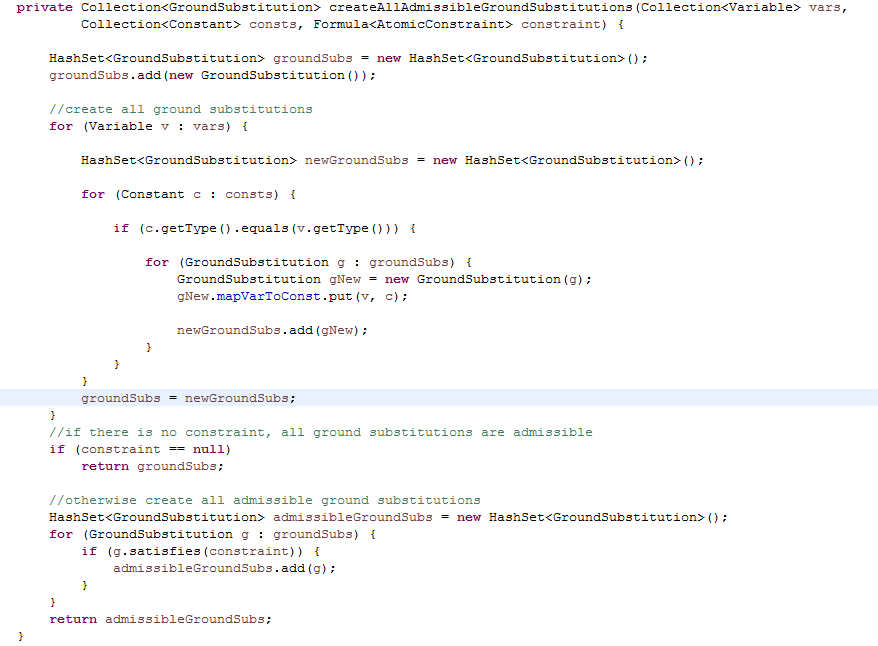
\includegraphics[scale = 1.0]{Graphics/Aenderung_1}
\begin{figure}[h]
	\caption{ConstraintBasedGroundingOperator}
\end{figure}


\section{Korrektur in Fraction}
Bei der Addition von zwei Objekten vom Typ Fraction kam es zu einem Überlauf.\\
In der Methode Fraction.addition wird das kleinste gemeinste Vielfache (least common multiple) benötigt. 
In der Methode Fraction.addition im Paket package edu.cs.ai.log4KR.math.types wird das kleinste gemeinste Vielfache (least common multiple) benötigt. 
Die Methode Fraction.lcm wurde ergänzt:\\
\\
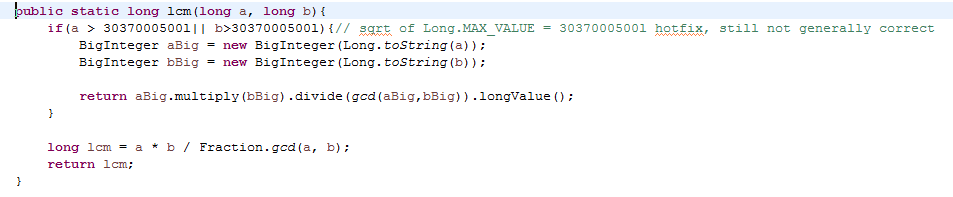
\includegraphics[scale = 1.0]{Graphics/Aenderung_221}
\begin{figure}[h]
	\caption{Fraction.lcd}
\end{figure}

Und die Methode Fraction.gcd wurde geändert von:\\
\\
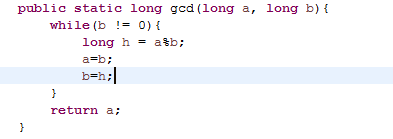
\includegraphics[scale = 1.0]{Graphics/Aenderung_211}
\begin{figure}[h]
	\caption{Fraction.gcd -alt-}
\end{figure}
\\
auf:\\
\\
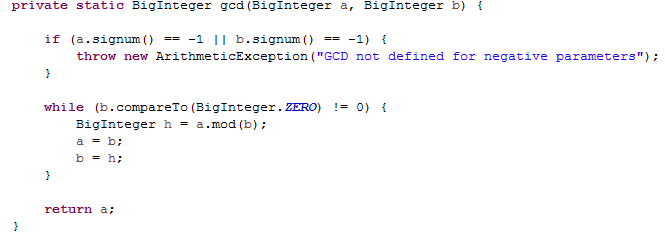
\includegraphics[scale = 1.0]{Graphics/Aenderung_212}
\begin{figure}[h]
	\caption{Fraction.gcd -neu-}
\end{figure}

\section{Modifikation von EqualityConstraint}
In der Klasse EqualityConstraint war nur die Methode EqualityConstraint.equals(Variable var, Term t) enthalten die einen Konstruktor aufruft statt Objekte zu vergleichen und der damit nicht in der in Collections üblicherweise vorgesehenen Weise agiert. Der Methodennamen erschient unglücklich gewählt.\\
Es wurde eine equals-Methode ergänzt, die die gewünschte Funktionalität zur Verfügung stellt.\\
\\
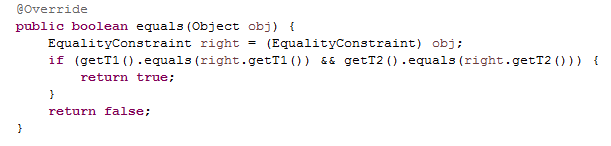
\includegraphics[scale = 1.0]{Graphics/Aenderung_3}
\begin{figure}[h]
	\caption{EqualityConstraint.equals(Object obj)}
\end{figure}


\section{Modifikation von InequalityConstraint}
Die Klasse InequalityConstraint enthielt keine equals-Methode.
Diese wurde ergänzt.\\
\\
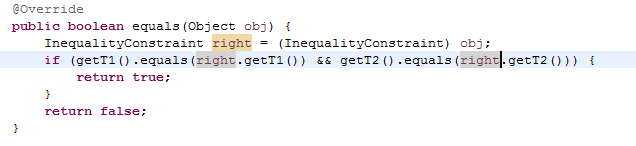
\includegraphics[scale = 1.0]{Graphics/Aenderung_4}
\begin{figure}[h]
	\caption{InequalityConstraint.equals(Object obj)}
\end{figure}


\section{Unbehandelter Fehler in Log4KR} \label{Fehler unbehandelt}
Beim Verarbeiten von mehr als einer spezifischen Konstante können Fehler auftreten. Die Beispiele wurden verworfen, eine Korrektur wurde nicht vorgenommen ist aber dringend anzuraten, sh. auch \ref{Beispiele unausfuehrbar} und \ref{examplesdep}.

\includegraphics[scale = 1.0]{Graphics/Beispiele_unausfuehrbar}
\begin{figure}[h]
	
\end{figure}




\chapter{Beispiele}
\label{examples}

\textbf{Vorbemerkung}

\noindent
Die folgenden Beispiele dienten der Gewinnung statistisch relevanten Materials und um die Problematik der Aufgabenstellung näher betrachten und erläutern zu können. Dabei wurden die Wahrscheinlichkeiten unter Verwendung von Log4KR berechnet. Die Eingabe der Wissensbasis erfolgte in der für Log4KR verwendbaren Form der FO-PCL Syntax. Zunächst wurden die Konditionale der Wissensbasis grundiert und deren jeweilige Wahrscheinlichkeit berechnet. Bei größeren Beispielen wurde hier auf die Ausgabe der Grundkonditionale aus Gründen der Übersichtlichkeit verzichtet.
Es wurden verschiedene Anfragen an die jeweilige Wissensbasis gestellt, die ebenso grundiert und mit der berechneten Wahrscheinlichkeit versehen wurden.
Anschließend wurde die angestrebte Ausgabe \index{angestrebte Ausgabe} generiert. 

\section{Birds} Erläuterungen s. \ref{BBirds}, eine Kurzversion des Beispieles findet sich unter \ref{Bsp:Birds}
\label{Birds}
\lstinputlisting{Examples/Birds.txt}
\newpage

\section{Birds2Birds} Erläuterungen s. \ref{BBirds2Birds}
\label{Birds2Birds}
\lstinputlisting{Examples/Birds2Birds.txt}
\newpage

\section{Birds2Classes} Erläuterungen s. \ref{BBirds2Classes}
\label{Birds2Classes}
\lstinputlisting{Examples/Birds2Classes.txt}
\newpage

\section{Birds3Classes} Erläuterungen s. \ref{BBirds3Classes}
\label{Birds3Classes}
\lstinputlisting{Examples/Birds3Classes.txt}
\newpage

\section{BirdsDiffer} Erläuterungen s. \ref{BBirdsDiffer}
\label{BirdsDiffer}
\lstinputlisting{Examples/BirdsDiffer.txt}
\newpage

\section{BirdsEqual} Erläuterungen s. \ref{BBirdsEqual}
\label{BirdsEqual}
\lstinputlisting{Examples/BirdsEqual.txt}
\newpage

\section{BirdsNot} Erläuterungen s. \ref{BBirdsNot}
\label{BirdsNot}
\lstinputlisting{Examples/BirdsNot.txt}
\newpage

\section{BirdsWithoutNull} Erläuterungen s. \ref{BBirdsWithoutNull}
\label{BirdsWihoutNull}
\lstinputlisting{Examples/BirdsWithoutNull.txt}
\newpage

\section{Cold} Erläuterungen s. \ref{BCold}
\label{Cold}
\lstinputlisting{Examples/Cold.txt}
\newpage


	\section{ColdSpez} Erläuterungen s. \ref{BColdSpez}
	\label{ColdSpez}
	\lstinputlisting{Examples/ColdSpez.txt}

\newpage


\section{ColdTrans} Erläuterungen s.  \ref{BColdTrans}
\label{ColdTrans}
\lstinputlisting{Examples/ColdTrans.txt}

\newpage

	\section{ColdTransSpez} Erläuterungen \ref{BColdTransSpez}
	\label{ColdTransSpez}
	\lstinputlisting{Examples/ColdTransSpez.txt}

\newpage


\section{Friendship} Erläuterungen s. \ref{BFriendship}
\label{Friendship}
\lstinputlisting{Examples/Friendship.txt}
\newpage

\section{FriendshipWithMisanthrope} Erläuterungen s. \ref{BFriendshipWithMisanthrope}
\label{FriendshipWithMisanthrope}
\lstinputlisting{Examples/FriendshipWithMisanthrope.txt}
\newpage

\section{Garfield}  Erläuterungen s. \ref{BGarfield}
\label{Garfield}
\lstinputlisting{Examples/Garfield.txt}

\newpage

\section{Misanthrope} Erläuterungen s. \ref{BMisanthrope}, eine Kurzfassung dieses Beispiel findet sich unter \ref{sec:Misanthrop}
\label{Misanthrope}
\lstinputlisting{Examples/Misanthrope.txt}
\newpage



\section{MisanthropeIrreflexive} Erläuterungen s. \ref{BMisanthropeIrreflexive}
\label{MisanthropeIrreflexive}
\lstinputlisting{Examples/MisanthropeIrreflexive.txt}
\newpage

\section{Monkeys2} Erläuterungen s. \ref{BMonkeys}
\label{Monkeys2}
\lstinputlisting{Examples/Monkeys2.txt}

\newpage

\section{MonkeysA} Erläuterungen s. \ref{BMonkeysA}
\label{MonkeysA}
\lstinputlisting{Examples/MonkeysA.txt}

\newpage

\section{Sport} Erläuterungen s. \ref{BSport}
\label{Sport}
\lstinputlisting{Examples/Sport.txt}
\newpage

\section{SportEx} Erläuterungen s. \ref{BSportEx}
\label{SportEx}
\lstinputlisting{Examples/SportEx.txt}
\newpage


\section{SportExN} Erläuterungen s. \ref{BSportExN}
\label{SportExN}
\lstinputlisting{Examples/SportExN.txt}


\newpage

\section{SportExNFam} Erläuterungen s. \ref{BSportExNFam}
\label{SportExNFam}
\lstinputlisting{Examples/SportExNFam.txt}


\newpage



\chapter{Verworfene Beispiele}
\label{examplesdep}
\textbf{Vorbemerkung}


\noindent
Die hier aufgeführten Beispiele konnten leider nicht getestet werden, da Log4KR keine entsprechenden Berechnungsmöglichkeiten zur Verfügung gestellt hat. Sie mussten daher verworfen werden. Die entsprechenden Fehlermeldungen sind unten stehend aufgeführt.

\section{Misanthrope2Spez} Erläuterungen s. \ref{BMisanthrope2Spez}
\label{Misanthrope2Spez}
\lstinputlisting{Examples/Misanthrope2Spez.txt}

\newpage


\section{Misanthrope3Spez} Erläuterungen s. \ref{BMisanthrope3Spez}
\label{Misanthrope3Spez}
\lstinputlisting{Examples/Misanthrope3Spez.txt}

\chapter{Änderungen gegenüber der letzten Version (wie besprochen)}

\setlength{\currentLongTableWidth}{\textwidth} %setze neue länge auf textbreite
\addtolength{\currentLongTableWidth}{-4\tabcolsep} %subtrahiere -8\cdot textbreite von asdf, 2 Abstände pro Zelle * Anzahl der Spalte
\begin{footnotesize}
	\begin{longtable}{ | p {0.5\currentLongTableWidth} | p {0.5\currentLongTableWidth}  |}
		\hline
		\multicolumn{2}{|c|}{\textbf{Änderungen in der Version}}\\\hline\hline
		\hline
		\textbf{Besprochene Änderung} 
		& \textbf{Umsetzung} 
		
		
		\endhead
		\hline
		\endfoot
		\endlastfoot
		\hline
		Definitionen sollten überarbeitet werden-, dazu gehören: 
		\newline spezifische Konstante, spezifisches Konditional
		& \newline \newline \ref{Konstanten spezifisch}\\
		\newline generische Grundinstanzen \newline  spezifische Grundinstanzen 
		&   \newline \newline \ref{Grundinstanz generisch} \newline \ref{Grundinstanz spezifisch} \newline \\
		Qualitatives Konditional
		& \ref{qualitatives_Konditional}\\
		Generalisierung, insbes. generalisiertes Konditional 
		&  \ref{Generalisierung}\\
		Ausgabe der Komponente
		& \ref{Ausgabe der Komponente}\\

		\hline
		Beispiele überarbeitet
		& sh.  \ref{Bsp:Generalisierung},  \ref{Bsp:Ausgabe der Komponente}  \ref{Bsp:Birds}\\
		\hline
		neu: Exkurs: Vergleich von Konditionalen überarbeitet
		&\ref{Ermittlung spezifischer Konstanten} \\
		\hline
		\caption{Änderungen gegenüber der letzten Version}
	\end{longtable}
\end{footnotesize}


\bibliography{FO-PCL_literatur}
\bibliographystyle{alphadin}
\addcontentsline{toc}{chapter}{Literatur}
\lhead{}




\renewcommand{\nomname}{Abkürzungs- und Symbolverzeichnis}
\thispagestyle{myheadings}
\markboth{}{ABKÜRZUNGS- UND SYMBOLVERZEICHNIS}
\printnomenclature
\addcontentsline{toc}{chapter}{Abkürzungs- und Symbolverzeichnis}
\newpage

\listoftheorems
\addcontentsline{toc}{chapter}{Liste der Sätze, Definitionen und Beispiele}
\newpage

\listoftables
\addcontentsline{toc}{chapter}{Tabellenverzeichnis}
\newpage

\listoffigures
\addcontentsline{toc}{chapter}{Abbildungsverzeichnis}
\newpage


\addcontentsline{toc}{chapter}{Index}
\printindex
\thispagestyle{myheadings}
\markboth{}{INDEX}
\newpage





\end{document}


